% Document
\documentclass[
    a4paper,
    12pt
]{extreport}
\usepackage[
    left=3cm,
    right=2.5cm,
    top=2.5cm,
    bottom=2.5cm,
    bindingoffset=1cm
]{geometry} % Better margin control
\usepackage[utf8]{inputenc} % Encoding (I think)
\usepackage{etoolbox} % Patching other packages (I think)
\usepackage{parskip} % Line spacing
\usepackage{setspace}
\usepackage[english]{babel}
\usepackage{hyperref}
\usepackage[toc,page]{appendix}
\usepackage[super,negative]{nth}
\usepackage{amssymb}
\usepackage{pifont}
\usepackage{enumitem}

% Figures and tables
\usepackage{mdframed}
\usepackage[font=scriptsize,skip=2pt]{caption}
\usepackage{subcaption}

% Figures
\usepackage{pdfpages}
\usepackage{graphicx}
\usepackage{xcolor}
\usepackage[many]{tcolorbox}
\usepackage{fancyvrb}
\usepackage{rotating}
\usepackage[outputdir=./_build]{minted}

% Tables
\usepackage{multirow}
\usepackage{array}
\usepackage{booktabs}
\usepackage{tabularx}
\usepackage{threeparttable}

% Bibliography
\usepackage{natbib}
\usepackage{bibentry}

% Remove spacing above \chapter head
\makeatletter
\patchcmd{\@makechapterhead}{\vspace*{50\p@}}{}{}{}
\patchcmd{\@makeschapterhead}{\vspace*{50\p@}}{}{}{}
\makeatother

% Set TOC numbering depth
\setcounter{tocdepth}{4}
\setcounter{secnumdepth}{2}

% Set font defaults
\setstretch{1.5}
\setlength{\parindent}{0em}

% Set hyperref defaults
\hypersetup{
    colorlinks,
    citecolor=black,
    filecolor=black,
    linkcolor=black,
    urlcolor=black
}

% Set BVerbatim defaults
\fvset{
    fontsize=\fontsize{9}{13},
    baseline=c
}

% Set list spacing
\setlist{nosep}

% Change 'Bibliography' to 'References'
\makeatletter
\def\thebibliography#1{\chapter*{References\@mkboth
  {REFERENCES}{REFERENCES}}\list
  {[\arabic{enumi}]}{\settowidth\labelwidth{[#1]}\leftmargin\labelwidth
\advance\leftmargin\labelsep
\usecounter{enumi}}
\def\newblock{\hskip .11em plus .33em minus .07em}
\sloppy\clubpenalty4000\widowpenalty4000
\sfcode`\.=1000\relax}
\makeatother

% Add Table column type (centered)
\newcolumntype{Y}{>{\centering\arraybackslash}X}

% Setup captions for figures
\captionsetup[figure]{
    font=normalsize,
    labelformat=empty,
    labelfont=bf,
    textfont=normalfont,
    singlelinecheck=off,
    justification=justified
}

% Setup captions for tables
\captionsetup[table]{
    font=normalsize,
    labelfont=bf,
    textfont=normalfont,
    singlelinecheck=off,
    justification=raggedright,
    labelformat=empty
}

% Set Minted environment
\setminted{
    breaksymbolleft=,
    fontsize=\fontsize{9}{13},
    baselinestretch=1.1,
    xleftmargin=2.5em,
    linenos,
    breaklines,
    tabsize=4
}

% Custom commands
\newcommand*{\mC}[2]{\multicolumn{1}{#1}{#2}}
\newcommand{\q}[1]{``#1''}
\newcommand{\cmark}{\ding{51}}
\newcommand{\xmark}{\ding{55}}

% Title
\title{CouchDB: A Data Adapter for Irregular Schemas}
\author{Zach Smith}
\date{\today}

% Document
\begin{document}

% Title page
\maketitle
\thispagestyle{empty}

% Abstract
\begin{abstract}
    CouchDB is a NoSQL database that shines when working with large semi/un-structured datasets such as are typically used in data mining. Data mining comprises ETL processes in which multiple datasets are joined, and explored in terms of projection (attribute filtering) \& selection (row filtering) before processing via machine learning. Looking at three datasets - UCT grades, student admission benchmarks and Learning Management System (LMS) usage, this project discusses the application of CouchDB within the data-mining process.

Due to the elegance with which CouchDB separates data storage/retrieval from entity modeling, CouchDB is an efficient tool for handling of large datasets with inconsistent schemas. In this project MapReduce is used to normalize data types during projection and to create indices of derived data suitable for performing joins and aggregations across multiple, different datasets. Using a List function (as provided by the CouchDB API), data from indices is iteratively retrieved, joined, and exported in CSV format for assessing attribute variance and correlations between different attributes.

In the context of the analyzed data, it is shown that academic performance of students taking the CSC1015F course correlates better with National Benchmark Tests (NBT) than to Grade 12 (matric) performance.
\end{abstract}
\newpage

%  TOC
\tableofcontents
\newpage
\listoffigures
\newpage
\listoftables
\newpage

% Content
\chapter{Introduction}
An understanding of the relationship between indicators such as student grades, online participation, engagement with assigned materials, or demographic information can allow for more adaptive pedagogical approaches to teaching and learning. As such, data mining the massive amount of information that learning management systems (LMS) – such as the University of Cape Town's (UCT) Sakai platform \cite{sakai} – collects has the potential to greatly improve the educational experience. Systems that support data-storage and retrieval are integral to the process of working with these datasets and the logical frameworks that guide the design of such systems are becoming increasingly important as the rate and amount of data collected continues to grow exponentially.

As the implementation and usage of data mining expands, alternatives to traditional relational-orientated databases are becoming the preferred software for housing large data stores. SQL systems such as Oracle, DB2, SQL Server, MySQL and others, tend to scale better vertically than horizontally \cite{couchbaseWhitePaper}. This can be limiting and expensive when compared to NoSQL databases, which allow for the seamless expansion from single to multiple servers.  But swapping out relational-storage for newer alternatives involves a mental shift at many levels within the software stack; this is most evident at the data-retrieval layer, with the shift from using SQL (structured query language) to query data stores to other paradigms that are less familiar to most data professionals (software engineers, software architects, database administrators, etc.). Although many NoSQL databases (databases that don't implement a relational model) implement a version of the SQL standard for querying (which eases the learning curve for new technologies), many do not.

One alternative paradigm to SQL is MapReduce, a logical framework for data querying that allows for the efficient processing of dispersed datasets. This technology, which is already used by several software giants \cite{chandar2010}, is being adopted as part of the new technology stack as part of the ongoing trend of ``information explosion''. As distributed computing power becomes more obtainable through the proliferation of cloud providers such as Digital Ocean, Hetzner, Amazon, Google, etc., it is worth investigating how technologies that make use of dispersed processing via the MapReduce paradigm can do relational operations such as joins, selections, and aggregations.

Also relevant to the shift from relational to non-relational databases is the increasing diversity of the data being collected digitally. As mentioned by the Couchbase project \cite{couchbaseWhitePaper} and observed from general experience in the modern workplace, much of the data produced on a day-to-day basis is semi-structured or unstructured (for example, text documents and spreadsheets). In turn, increasing technological gains, such as those represented by the proliferation of IOT (internet of things) devices, require the housing of ever more varied digital data. RDBMSs seem ungainly in this scenario, with their strictly defined data models making it cumbersome to handle semi-structured and unstructured data. Appropriate systems are expensive in terms of implementation times and complex in terms of architecting and usage. Storing data without having to first define rigid models allows for a more agile approach to data modeling.  Additionally, as a system evolves, subsequent changes to unstructured data models become straightforward and the knock-on effects of code-changes are much more isolated.

\section{Project Significance}
CouchDB is a new technology that embodies much of the NoSQL trend: it has a schema-less data model; it accomplishes data processing via MapReduce; it exists as an open-source code-base, and it is suitable for distribution over commodity hardware.

As an example of CouchDB implementation, this project enables the further development of CouchDB-based applications. With a focus on highly available data and a replication API implemented across multiple types of devices (servers, browsers, tablets, mobile phones, etc.), CouchDB provides a suitable foundation for building offline-first applications that can be used in relatively disconnected locations \cite{ebola2017}. For example, CouchDB was deployed as part of the effort to contain the 2013 - 2016 Ebola outbreak, providing a means of digital data collection in areas with unreliable internet \cite{ebola2017}. Similarly, there is a lot of scope for offline-first application development in the South African context, where data is still very expensive and internet access remains sporadic throughout much of the country.

In terms of this specific case study, insight into joins, selections and aggregating data using CouchDB is discussed in the context of Educational Data Mining (EDM). The effectiveness of UCT's student profiling during the admissions process is discussed in relation to performance in the first-year Computer Science course, CSC1015F, and a means of correlating students’ usage of the Sakai LMS and final course grades is tested.

\section{Motivation \& Aim}
Theoretically, CouchDB is suitable for storing an unlimited amount of unstructured data across distributed clusters of commodity servers \cite{couchdb2.0}. An API that is effectively an interface for the manipulation of b+tree structures is a novel approach to data handling and working with the database directly from an HTTP client is incredibly convenient. Such features make CouchDB a suitable tool for the information-orientated society of the future, where an agile approach to data storage will, by necessity, become the norm as the increasingly interconnected world will produce more and more unstructured data needing to be processed.

In short, CouchDB is an innovative database that allows for innovative systems. Case studies involving CouchDB are therefore necessary to develop an understanding of all the different use-cases that such novel software can represent.

The aim of this project is to provide a CouchDB case study in terms of handling relational data.

\chapter{Background}
Any data-driven investigation requires learning of a variety of tools and concepts. This chapter covers:

\begin{itemize}
    \item A conceptual overview of MapReduce as a paradigm for working with data, and its specific implementation in CouchDB - the primary means of data-retrieval using CouchDB
    \item A high-level description of the CouchDB storage engine and approaches to structuring/modeling data in a document-orientated database
    \item A brief description of CouchDB's HTTP API
    \item Context of this project in terms of EDM
\end{itemize}
\section{MapReduce}
In response to dealing with huge amounts of data on a daily basis, authors at Google (Jeffrey Dean and Sanjay Ghemawat) outlined a programming model that abstracted complications associated with distributed computing such as how to parallelize processing, data distribution, fault tolerance, load balancing and execution time \cite{Dean:2008}. This model, known as \textit{MapReduce}, provides programmers a conceptually-simple interface for specifying dispersed data computations succinctly and hides implementation details. The framework relies on an astoundingly simple programming model described by \cite{Dean:2008} as a computation that takes a set of input \textit{key:value} pairs and produces a set of output \textit{key:value} pairs via the following 3 steps:

\begin{itemize}
    \item A \textit{mapping} stage in which distributed \textit{key:value} pairs are produced from input data as described by a user-defined \textit{map} function
    \item A \textit{grouping} stage where distributed \textit{key:value} output from the mapping stage is collected to common \textit{keys} - i.e. \textit{key:[value, value, value]} datasets
    \item And a \textit{reduce} stage where \textit{values} per key \textit{key} are processed as described by a user-defined \textit{reduce} function
\end{itemize}

Due to the distributed and isolated nature of \textit{map} and \textit{reduce} tasks, \textit{MapReduce} as an idea is greatly fault tolerant (fault tolerance is implemented via reexecution), which has in turn resulted in the "New Software Stack" as mentioned by \cite{mining2011}: large scale computing clusters built on commodity (cheap) hardware and software that computes in parallel. The "New Software Stack" represents processing ever-greater amounts of data at ever cheaper rates and has spurred information explosion across all manner of software applications.

With the development of the \textit{Hadoop} framework as an open-source alternative to Google's proprietary file system and MapReduce framework, data computations within a MapReduce context have become mainstream. As \cite{chandar2010} discusses in his MSc thesis "Join Algorithms using Map/Reduce" made available by the University of Edinburgh, many companies now utilize this idea including Yahoo, Facebook, Amazon and many others (The Apache Foundation maintains a list of companies that use the Hadoop framework \cite{hadoopPower:2017}).

Many of the algorithms required on a day-to-day basis in common data-querying tasks can be implemented via the MapReduce framework including \textit{relational-algebra} operations such as \textit{selection}, \textit{projection} (selection of a subset of attributes from a tuple), \textit{union}, \textit{intersection}, \textit{difference}, \textit{joins} (non-equi joins cannot be implemented via MapReduce), \textit{grouping} and \textit{aggregation} \cite{mining2011}.

As the subject of his thesis, \cite{chandar2010} outlines and measures performance for \textit{Multi-Way} joins using \textit{Map-Side Join}, \textit{Reduce-Side One-Shot Join},\textit{Reduce-Side Cascade Join} algorithms. One take from this research is that both \textit{Two-Way} and \textit{Multi-Way} joins can be implemented via the MapReduce framework in general, though this is dependent on specific implementations and context of MapReduce engines.

MapReduce as implemented in the CouchDB software is used as a means of creating 'views' of databases, structured as indexes. Discussing CouchDB's MapReduce implementation in terms of relational operations is relevant since views often require some kind of relational grouping.
\section{CouchDB}
In CouchDB, data is modeled conceptually as \textit{documents}, which users interact with as serialized JSON strings \cite{rfc7159}. There are no limitations, specifications, etc., on how documents may be structured (other than that they must be represented by valid JSON). These comprise key-value pairs, in which the value may be derived from the objects themselves.

The CouchDB data model (like many NoSQL data models) is considered \textit{unstructured} or \textit{semi-structured} when compared to RDBMSs, where relations within data models are rigidly formalized. But despite using different storage models, the conceptual requirements of data-persistence – such as ACID properties – need to be addressed. ACID properties provide certain guarantees that are required within a system in order to assure information persistence:

\begin{itemize}
    \item \textit{atomicity}: a series of operations that are part of the same logical transaction should either succeed or fail completely
    \item \textit{consistency}: building on the concept of atomicity, the result of a single logical transaction should leave the database in a working and valid state
    \item \textit{isolation}: Transactions, whether run concurrently or sequentially, are deterministic. That is, transactions on a database are performed in isolation of each other
    \item \textit{durability}: data is permanently persisted, irrespective of subsequent system failures
\end{itemize}

Without such guarantees a database would not be useful since the integrity of any information stored the system would be questionable. In terms of the CouchDB software, ACID properties are applicable at the document level, meaning that the interactions with individual documents are either successful or not; CouchDB does not allow the reading or writing of partial documents.

CouchDB serializes document interactions to guarantee isolation and document writes are guaranteed to be durable and result in a consistent database. In other words, in working with CouchDB, transactions involving single documents are completely reliable and fault tolerant; however, transactions involving retrieving and storing information from multiple documents are not (although bulk document insertions can also be configured atomically).

Single-document ACID guarantees make multistep transactions in CouchDB more difficult. \textit{Multi-step transactional atomicity} is a key feature for many RDBMSs including MySQL, SQL Server, etc., and overcoming this limitation is required in order to implement NoSQL databases within traditional RDBMS environments. This is possible, both in CouchDB specifically \cite{Rashmi2017} and in NoSQL generally, \cite{LOTFY2016133} via the implementation of ACID/transactional properties as external bespoke middleware that engages with the database management systems (DBMS). But this is not an ideal alternative to systems where RDBMS-specific features are required. This is a trade-off that CouchDB (and other NoSQL) databases make in favor of less rigorous data models that are suitable for use-cases that RDBMSs are not; namely, environments with semi-unstructured data where availability is more important than complete consistency.

CouchDB documents are written to disc using an \textit{append-only} algorithm, in which documents are incorporated into a b+tree structure, which is the database \cite{couchguide}. Such structures facilitate rapid data retrieval from huge databases. Additionally, CouchDB incorporates \textit{Multiversion concurrency control} (MVCC) into the storage engine as a means of versioning nodes within the tree. Aside from the serialization of write operations, MVCC negates the need for locks, which are typically implemented within RDBMSs and are expensive in terms of computer resources. Without locking on read/write operations, CouchDB data stores are always available, with the caveat that retrieved documents, as found through searching the tree structure, may not always be the most recent versions of those documents. This can be the case if a new version of a document is written whilst the same document is being retrieved elsewhere.

For systems faced with the potential of network downtime, research in 1999 introduced the idea of the CAP theorem as a trade-off analysis that can be applied to 3 properties within a data storage system (Consistency, Availability, and Partition-tolerance) \cite{cap}. CouchDB represents a trade-off of \textit{consistency} for \textit{availability} in order to facilitate scalability in terms of handling large amounts of data in nearly real time. CouchDB emphasizes availability and the eventual consistency of data to allow for a high partition tolerance of databases with unreliable communication between nodes. From CouchDB 2.0 onwards, users can configure the level of consistency for document reads by specifying a quantifiable amount of confidence that retrieved data is not out of date. It should be noted, however, that this is not possible for document writes.

Because of the potential for inconsistency, CouchDB seeks to provide a 'relaxed' viewing model - i.e. a \textit{soft state}, where data representation is not tied to the underlying entities. As part of the trade-off of availability at the expense of consistency, data conflicts - where entities are updated separately and independently of each other - are often acceptable in NoSQL databases, particularly in systems that are required to take an \textit{offline-first} approach to data-handling. Thus, these systems provide a means of interacting with partial datasets, which, when synchronized, could result in a conflicting state.

MVCC allows for the handling of such consistency violations by maintaining consistency within the data storage layer itself, which is separate from the consistency of information. Inconsistent (i.e. conflicting) information can be resolved by following the audit trail created by the MVCC mechanism. By maintaining a database state that is separate from the information-state, multi-master replication in highly-available systems that lack strong consistency guarantees is possible.

CouchDB is usually selected as a database over alternative JSON stores (such as MongoDB) for its replication capabilities - that is, for the ease with which multi-master, fault-tolerant clusters can be set up. The separation of the database state from the information greatly facilitates this. Compared to replication within relational systems (such as in SQL Server), here replication is independent of information (i.e. table structure, relationships between tables, etc.) and, as a result, is much simpler to work with.

\subsection{Entity Modeling}
Despite NoSQL DBMSs moving away from the relational model provided by RDBMSs, data models still focus on modeling entities. Depending on what these entities constitute, the databases can be grouped into two categories \cite{fowlerAggregate}:

\begin{itemize}
    \item \textit{aggregate-orientated} stores that model data similarly to the relational model, but with isolated entity boundaries and
    \item \textit{aggregate-ignorant} stores, wherein the concept of entities is fundamentally different (e.g. a graph database such as Neo4J \cite{sadalage2012}, where the entities are edges and nodes)
\end{itemize}

Most databases operate within a domain where data is, for the most part, entity-driven. There are hundreds of NoSQL data stores and a comprehensive catalog of such products is not necessary \cite{GANESHCHANDRA201513}, but familiar examples within the family of aggregate-orientated NoSQL databases include key-value stores such as Amazon's Dynamo \cite{sadalage2012}; column based stores such as Apache's Cassandra \cite{sadalage2012} or HBase \cite{sadalage2012} (as part of the Hadoop ecosystem); and document stores such as CouchDB or Mongo \cite{sadalage2012}.

Although NoSQL databases are said to be \textit{schema-less}, this is something of a misnomer \cite{ATZENI2016}: NoSQL databases allow for inconsistent schema representation across different entity instances due to the nature of how entities are enforced. Such flexibility is at the heart of document stores such as CouchDB and Mongo, where loose-schema modeling is one of the properties that makes such technologies suitable for large systems that generate data from inconsistent sources.

JSON structure allows for forming hierarchical (tree) structures of infinite depth - i.e. for nesting child entities as sub-objects. As an alternative to relationships that are defined by key references, hierarchical structures allow for the easy structuring of specific entities but are less suitable for working with classes of entities. As such, data is typically grouped differently in JSON documents as compared to relational tables; objects encourage groupings of specific entities, while tabular relations encourage the grouping of entity types.

Using hierarchical object structures, it is easy to implement compositional object models, where entities are encapsulated exclusively within parent entities. Aggregational and associative relationships (i.e. \textit{many-many} associations), however, require that data be denormalized, which results in replicated information. This is inefficient but advantageous for dealing with entities whose instances have varying data structures. For example, it is conceivable that the instance of a \textit{Person} entity could have different fields, with similar fields holding different types of data (e.g., a person may have a single address or a list of addresses).

To think of entities as rows within a relational table, each entity represented via JSON is allowed a unique list of columns featuring differing data types as values. In a relational database this would result in a sparse table where every row must include the columns of every other row of the same entity type. Such a case would result in a massive amount of wasted storage and inefficient indexing.

Entity modeling in CouchDB is quite flexible. RDBMSs allow for the categorization of information in terms of relations, fields, constraints, and other objects, while MongoDB documents are identifiable in terms of \textit{collections}. CouchDB does not provide a built-in means of classifying documents, except by scanning an entire database and reading each document.

Entity classification can be enforced by including a field \textit{type} that allows for entity modeling to be conducted separately from the data-storage engine. With this approach, documents are only classifiable on retrieval and deserialization. Alternatively, entity classification can be included in the \textit{\_id} field of CouchDB documents, which has the benefit of allowing for indexed entity retrieval.
\subsection{API}
\subsubsection{HTTP Interface}
All communication with CouchDB takes place via the HTTP protocol. The interface is resource orientated and strives to be RESTful. This makes such interactions very clear since the HTTP endpoints are logical and easy to remember. For example, the following sample endpoints (among many) are shown here, though the full API is very well documented online \cite{couch-api}.

\begin{itemize}
    \item \textit{GET} /dbName/:id (retrieves a document with the specified ID)
    \item \textit{PUT} /dbName/[:id] (inserts a document, optionally specifying an ID)
    \item \textit{POST} /\_bulk\_docs (inserts multiple documents - atomicity of batch insert is configurable but defaults to false)
    \item \textit{POST/GET} /\_all\_docs (Fetches multiple documents, specifying keys can be done in in the body of a post request)
\end{itemize}

\subsubsection{Design Documents}
CouchDB allows users to specify several different types of functions that can be executed on the server-side Erlang application via JSON - as a regular database document, but with an \textit{\_id} of ``\_design/$<$name$>$''. Such documents are known as \textit{design} documents and are treated as special by the CouchDB application. CouchDB executes functions that are defined in design documents on the server - functions can be defined in a variety of languages, including JavaScript. There are 6 types of functions that users can define for server-side execution:

\begin{itemize}
    \item \textit{views}
    \item \textit{shows}
    \item \textit{lists}
    \item \textit{updates}
    \item \textit{filters}
    \item \textit{validations}
\end{itemize}

Views are b+tree indexes created by specifying a mapping function and an optional reduce function to be executed on every document in a database. Map functions iteratively take each document as an argument and output key-value pair(s) - as specified by the Map function definition - that are then incorporated into the b+tree. Reduce functions are evaluated by taking Map-function outputs as inputs and returning reduced results from that input, which are stored as internal nodes on the b+tree.

Show functions act as a type of middleware, allowing users to specify transformations on a single document that has been requested from the database and then returning that document to the user - for example, transforming a document from JSON representation to HTML representation for better display in a browser. List functions are similar to show functions, but they transform sets of documents that have been iteratively retrieved from an index instead of single documents that have been retrieved from a database.

Update functions allow document updates to be performed indirectly via the HTTP API (functionally equivalent to retrieving a document, updating it, and then reinserting it). Filters, true to their name, allow users to specify filters that can be used during view retrieval, document retrieval, and in replicating data between CouchDB databases. Validations allow users to specify rules regarding when a database’s documents can be updated and by whom.

\subsection{Indices (Views)}
Essentially, CouchDB provides users a simple-to-use HTTP interface that allows for fine-grained control over b+tree structures. Documents can either be retrieved from trees directly or indices can be built as representations of databases using MapReduce and then retrieved. Index creation involves iteratively processing every document in a database and outputting a new b+tree structure (and index), providing a \textit{view} of the underlying database. Views provide a means for applying selections, projections, and aggregations of databases.

In the current CouchDB release (as of January 2018), there is an additional means of querying CouchDB databases called `Mango', which is a selection-based syntax inspired by MongoDB. The Mango syntax still processes documents via MapReduce, but it is generally faster than JavaScript functions since the MapReduce engine can be executed directly within the Erlang process on the server.

Map functions must be specified by a user and are always executed externally to the main Erlang process via marshalling between the main Erlang process and the indexing engine. Reduce functions, however, can either by executed via the main Erlang process (by specifying a built-in reduce function) or externally by the indexing engine when specifying custom reduce functions. CouchDB automatically includes a MapReduce engine (\textit{couchjs.exe}), which is a JavaScript query-server (indexing engine) coupled with Mozilla's SpiderMonkey runtime engine. This query engine is replaceable by dropping in alternative implementations in JavaScript or other languages, if required. CouchDB spawns a single couchjs.exe process per shard and executes map/reduce functions in the context of new documents sequentially according to the order in which the database was changed \cite{slack2Nov,slack7Nov}.

Conceptually, \textit{fetching all documents of type x} requires specifying an iteration through every document in the database and fetching documents with content indicative of type \textit{x}. View indices are built into CouchDB in this fashion, via iterating over every document in the database, and passing that document to the user-defined map function. A user writes code in this map function that evaluates each document and emits key-value pairs. The map output is then grouped by key and passed to the reduce function for reduction.

Users can specify whether they want to retrieve reduced results or access the unreduced map results (meaning, a reduce function isn't actually required to produce a CouchDB view). However, when passing output from the map function to the reducer, where map output is grouped by key, there is no guarantee that all the map output for a particular key will be sent to the same reduce function \cite{reduceFunctions}. As such, a reduce function may repeatedly operate on the same output as the map function, necessitating the `rereduction' of already reduced output. The reduce function requires handling in cases where \mintinline{text}{rereduce=true} and \mintinline{text}{rereduce=false} within the same function body. Therefore, writing custom reduce functions that adhere to the reduce function contract is fairly difficult for anything other than the simplest of examples. CouchDB's reduce function contract is as follows:

\begin{itemize}
    \item \textit{keys}: a list of tuples of the form of \textless \textit{key}, \textit{id} \textgreater. \textit{key} is the key emitted by the map function defined by the user and \textit{id} is the ID of the document that was processed by the map function in order to emit the key (this is implicit and not defined by a user). This argument is null in the case of \mintinline{text}{rereduce=true}.
    \item \textit{values}: a list of the values emitted by the map function as defined by the user, with each value correlating to the respective element in the keys list (when \mintinline{text}{rereduce=false}). When \mintinline{text}{rereduce=true}, this argument is a list of values that were output previously by this same reduce function on an earlier execution.
    \item \textit{rereduce}: a boolean field indicating whether the function is invoked with output from the map function (\mintinline{text}{rereduce=false}) or with previous output from the reduce function (\mintinline{text}{rereduce=true}). Reduce function results are cached on internal nodes in the b+tree view indexes to facilitate incremental tree updates without requiring the recalculation of all reduce output \cite{slack25Oct}, making the rereduce contract necessary.
\end{itemize}

\subsubsection{\textit{\_sum} Reduce Function}
Adherence to the contract of the \_sum reduce function requires that values output by the map function are either numerical or a list of numerical values - examples of both allowable map function output formats are shown in Figure \ref{fig-sum-reduce-fn} A. The reduce function receives values grouped by key (Figure \ref{fig-sum-reduce-fn} B) as the \nth{2} argument during execution. The reduce function signature is shown in Figure \ref{fig-sum-reduce-fn} C; the \nth{1} argument is a separate list of grouped key-id pairs for every document that output a specific key, and the indices of the \nth{1} argument correspond to indices in the \nth{2} argument (list), in terms of which document produced which value.

Figure \ref{fig-sum-reduce-fn} D shows the logical treatment of the grouped values by the \_sum function; for a list of values of the same key, values at corresponding indices are summed. In the case where an index is out of bounds (when grouped values differ by list length, or when some values are numerical and others are lists), the value '0' is used. Output of the \_sum function is shown in Figure \ref{fig-sum-reduce-fn} E.

\begin{figure}[H]
    \centering
    \begin{mdframed}[rightline=true,leftline=true]
        \begin{minted}{text}
/* A: Map output*/
{["key"]: 7} // (_id: x)
{["key"]: [3,1,3]} // (_id: y)
{["key2"]: [2,2,2]} // (_id: z)

/* B: Map output grouped by key */
{["key"]: [7,[3,1,3]]}
{["ke2"]: [[2,2,2]]}

/* C: Map output passed to _sum function as input */
reduce([key:id tuples], [values groupted by key], rereduce)
reduce([["key", "x"], ["key", "y"]], [7,[3,1,3]], false)
reduce([["key2", "z"]], [[2,2,2]], false)

/* D: Logical treatment of values argument (arg 2) during reduction */
{["key"]: [sum([7,3]), sum([0,1]),  sum([0,3])]}
{["key2"]: [sum([2]), sum([2]),  sum([2])]}

/* E: Reduce output (group = true) */
{
  ["key"]: [10, 1, 3],
  ["key2"]: [2,2,2]
}
    \end{minted}
    \end{mdframed}
    \caption[\_sum Reduce Function Logic]{\textbf{Figure \ref{fig-sum-reduce-fn}: Logical description of the \_sum Reduce function contract shown as a step-based series of transformations from input (map function output) to output}}
    \label{fig-sum-reduce-fn}
\end{figure}

\subsubsection{\textit{\_stats} Reduce Function}
To adhere to the \_stats function contract, key-value output by the map function should follow specific constraints:

\begin{itemize}
    \item All values must be a single number
    \item Or, all values must be an array of numbers (each array must be the same length). An example of this format is shown in Figure \ref{fig-stats-reduce-fn} A
\end{itemize}

This is unlike the contract for the \_sum function, where value output is \textit{normalized} during the reduction of lists of unequal length or the reduction of lists and numerical values. The aggregation of grouped of values (as shown in Figure \ref{fig-stats-reduce-fn} B) is completed by the \_stats function. For values that are groups of numbers (i.e. where the map function outputs key-number) then a single \_stats object is output for each unique key. Map output is received as input to the \_stats reduce function within 3 parameters as shown in Figure \ref{fig-stats-reduce-fn} C:

\begin{itemize}
    \item A list of \textit{MapOutputKey}:\textit{Document ID} key-value pairs (all the keys are the same, but the documents that \textit{emitted} them are different)
    \item A list of values for a particular key
    \item true / false (rereduction)
\end{itemize}

The values (argument 2 for the reduce contract) are aggregated by grouping them at common indices and reducing to a single \textit{\_stats object} as shown in \ref{fig-stats-reduce-fn} D. (Or, if the map output was a single number and not a list of numbers, the output becomes an aggregation of those numbers). If the values as output by the map function are lists of lists (of numbers), then a list of \_stats objects is output by the \_stats function as shown in Figure \ref{fig-stats-reduce-fn} E (one \_stats object per index within the list). The object output by the \_stats function for each aggregated number includes a count of how many items are included in the aggregation, the minimum value, the maximum value, the sum of all the values, and the sum of the squares of all the values. The output of the \_stats function includes output of both the \_sum and \_count built-in reduce functions. However, the stricter contract (when all values are lists of the same length or are numerical) makes this function cumbersome to use when only a sum or count is required.

\begin{figure}[H]
  \centering
  \begin{mdframed}[rightline=true,leftline=true]
    \begin{minted}{text}
/* A: Map output*/
{["key"]: [1,1,0]} // (_id: x)
{["key"]: [3,1,3]} // (_id: y)
{["key2"]: [2,2,2]} // (_id: z)

/* B: Map output grouped by key */
{["key"]: [[1,1,0],[3,1,3]]}
{["ke2"]: [[2,2,2]]}

/* C: Map output passed to _stats function as input */
reduce([key:id tuples], [values groupted by key], rereduce)
reduce([["key", "x"], ["key", "y"]], [[1,1,0],[3,1,3]], false)
reduce([["key2", "z"]], [[2,2,2]], false)

/* D: Logical treatment of values argument (arg 2) during reduction */
{["key"]: [aggregate([1,3]), aggregate([1,1]),  aggregate([0,3])]}
{["key2"]: [aggregate([2]), aggregate([2]),  aggregate([2])]}

/* E: Reduce output (group = true) */
{
  ["key"]: [
    {"sum":4,"count":2,"min":1,"max":3,"sumsqr":10},
    {"sum":2,"count":2,"min":1,"max":1,"sumsqr":2},
    {"sum":3,"count":2,"min":0,"max":3,"sumsqr":9}
  ],
  ["key2"]: [
    {"sum":2,"count":1,"min":2,"max":2,"sumsqr":4}
  ]
}
    \end{minted}
  \end{mdframed}
  \caption[\_stats Reduce Function Logic]{\textbf{Figure \ref{fig-stats-reduce-fn}: Logical description of the \_stats Reduce function contract shown as a step-based series of transformations from input (map function output) to output}}
  \label{fig-stats-reduce-fn}
\end{figure}
\section{Educational Data Mining}
Falling under the umbrella category of \textit{Educational Data Mining} (EDM), much work has been done with the intent of modeling student performance as dependent on certain markers such as attendance, assignment and test grades, high school marks, demographic data, etc. Different means of model generation have been discussed by the EDM community such as predictive analysis via decision tree generation \cite{Qasem20016,Balestra2017,casper2017,Dimitris,zebun2005,Mierle:2005} with varying results. Many other models have been applied within the field of EDM as discussed in a review of EDM up to 2009 \cite{bakerEdMiningSummary}.

Although these studies discuss analysis-frameworks at length, very little work has been done on the underlying data stores that form a basis of such analysis. As such, it appears that the work done so far looks to research feasible models in terms of accuracy and implementation rather than feasible means of implementing such mining techniques. Where \textit{Extraction, Transformation, and Loading} (ETL) processes have been discussed with regards to data preparation, SQL is used but without much discussion as to the implementation of the underlying relational data stores (\cite{Balestra2017,casper2017,Mierle:2005}). No attempts have been made to use newer and less conventional NoSQL stores such as CouchDB despite that benefit that such data stores provide in terms of the unique features that these newer data stores offer (\textit{schema-less} entites, easier scaling, lower costs of implementation and licensing, etc.).

\chapter{Data}
\label{chapter:data}
The focus of this project is the manipulation of data using CouchDB and associated technologies, whilst specifically using data from the business domain of Educational Data Mining (EDM). This field is well developed and many studies have sought to model student performance based on markers such as attendance, assignment and test grades, high school marks, demographic data, etc. Different means of model generation have been discussed by the EDM community, such as predictive analysis via decision tree generation \cite{Qasem20016,Balestra2017,casper2017,Dimitris,zebun2005,Mierle:2005}, with varying results. Other models have been applied within the field of EDM, as discussed in a review of EDM up to 2009 \cite{bakerEdMiningSummary}.

UCT’s Chief Information Officer (CIO) Jane Hendry and Stephen Marquard (the Learning Technologies Coordinator from the Center for Innovation in Learning and Teaching at UCT), made anonymized student data available for use in the present study. This encompasses UCT admissions data, course grades, and Sakai interactions. The three separate datasets are classified as:

\begin{itemize}
    \item \textit{grades}: UCT course results
    \item \textit{admissions}: Student Grade 12 and National Benchmark Test (NBT) results
    \item \textit{events}: Student interactions with the Sakai platform, measured as browser interactions
\end{itemize}

All three datasets are in CSV format and have the student number field in common, which has been anonymized consistently across all three datasets to preserve row associations.

\section{Grades}
Three years of data are available (2014, 2015, and 2016) and were received as separate CSV files, then compiled into a single file with normalized delimiters. The fields in the compiled file are described in Table \ref{tbl-data-grades}, and a sample of this file is shown in Figure \ref{fig-sample-grades}. Essentially this data comprises a list of the grades achieved for specific courses in specific years, along with the anonymized student numbers. The individual files could have remained separate, but for the purposes of this investigation it is easier to work with a single file rather than multiple files.

\begin{table}[H]
    \begin{threeparttable}
        \textbf{Table \ref{tbl-data-grades}}\par\medskip\par\medskip
        \caption[Grades data fields]{Grades data fields}
        \label{tbl-data-grades}
        \begin{tabularx}{\textwidth}{>{\hsize=0.8\hsize}X>{\hsize=0.6\hsize}X>{\hsize=1.6\hsize}X}
            \toprule
            \mC{c}{Field Name} & \mC{c}{Data type} & \mC{c}{Description}                              \\
            \midrule
            DownloadedDate     & date              & Excel date format                                \\
            RegAcadYear        & number            & Year                                             \\
            RegTerm            & number            & Integer ID                                       \\
            anonIDnew          & number            & Student number\tnote{\textsuperscript{1}}        \\
            RegProgram         & string            & Program abbreviation                             \\
            RegCareer          & string            & Academic level                                   \\
            Degree             & string            & Degree code                                      \\
            DegreeDescr        & string            & Degree title                                     \\
            Subject            & string            & Three letter abbreviation                        \\
            Catalog.           & string            & Catalog sub-component\tnote{\textsuperscript{2}} \\
            Course             & string            & Full course code description                     \\
            CourseSuffix       & string            & Course session identifier                        \\
            Session            & string            & Session name                                     \\
            Percent            & string            & Grade achieved by student                        \\
            Symbol             & string            & Symbol achieved by student                       \\
            UnitsTaken         & number            & Total units taken by student                     \\
            CourseID           & number            & Numerical course Identifier                      \\
            CourseDescr        & string            & Description of course                            \\
            CourseCareer       & string            & Academic level of course                         \\
            Faculty            & string            & Course faculty                                   \\
            Dept               & string            & Faculty department                               \\
            MaximumCrseUnits   & number            & N/A                                              \\
            CourseCount        & number            & N/A                                              \\
            CourseLevel        & number            & N/A                                              \\
            CESM               & number            & N/A                                              \\
            Sub-CESM           & number            & N/A                                              \\
            \bottomrule
        \end{tabularx}
        \scriptsize
        \begin{tablenotes}
            \item[\textsuperscript{1}]Anonymization was performed by Associate Professor Sonia Berman
            \item[\textsuperscript{2}]Course number and session identifier
        \end{tablenotes}
    \end{threeparttable}
\end{table}
\begin{sidewaysfigure}
  \centering
  \begin{mdframed}[topline=false,rightline=false,leftline=false]
    \centering
\begin{BVerbatim}
+--------+-------------+---------+----+------------+-----------+--------+-------------+---------+----------+----------+--------+--------------+--
| DnldDt | RegAcadYear | RegTerm | ID | RegProgram | RegCareer | Degree | DegreeDescr | Subject | Catalog. |  Course  | Suffix |   Session    |
+--------+-------------+---------+----+------------+-----------+--------+-------------+---------+----------+----------+--------+--------------+--
| txt    |        2016 |    1161 |  1 | CB003      | UGRD      | QCB007 | txt         | MAM     | 1000W    | MAM1000W | W      | Full Year    |
| txt    |        2016 |    1161 |  1 | CB003      | UGRD      | QCB007 | txt         | CSC     | 1015F    | CSC1015F | F      | Semester One |
| txt    |        2016 |    1161 |  2 | CB004      | UGRD      | QCB002 | txt         | CSC     | 1015F    | CSC1015F | F      | Semester One |
| txt    |        2016 |    1161 |  3 | EB022      | UGRD      | QEB028 | txt         | EEE     | 2036S    | EEE2036S | S      | Semester Two |
| txt    |        2015 |    1151 |  3 | EB022      | UGRD      | EB28   | txt         | CSC     | 1015F    | CSC1015F | F      | Semester One |
| txt    |        2016 |    1161 |  4 | CB004      | UGRD      | QCB002 | txt         | CSC     | 1015F    | CSC1015F | F      | Semester One |
| txt    |        2015 |    1151 |  4 | CB003      | UGRD      | CB07   | txt         | CSC     | 1015F    | CSC1015F | F      | Semester One |
| txt    |        2015 |    1151 |  5 | CB003      | UGRD      | CB07   | txt         | CSC     | 1015F    | CSC1015F | F      | Semester One |
+--------+-------------+---------+----+------------+-----------+--------+-------------+---------+----------+----------+--------+--------------+--
--+---------+--------+------------+----------+------------+-----------+---------+------+--------------+-----------+-----------+------+----------+
  | Percent | Symbol | UnitsTaken | CourseID | CourseDesc | CourseCrr | Faculty | Dept | MaxCrseUnits | CrseCount | CrseLevel | CESM | Sub-CESM |
--+---------+--------+------------+----------+------------+-----------+---------+------+--------------+-----------+-----------+------+----------+
  |      71 | 2+     |         36 |   107088 | txt        | UGRD      | SCI     | MAM  |           36 |         1 |        41 | 1501 |        1 |
  |      70 | 2+     |         18 |   103034 | txt        | UGRD      | SCI     | CSC  |           18 |       0.5 |        41 |  606 |        6 |
  |      55 | 3      |         18 |   103034 | txt        | UGRD      | SCI     | CSC  |           18 |       0.5 |        41 |  606 |        6 |
  |      63 | 2-     |         12 |     1642 | txt        | UGRD      | EBE     | EEE  |           12 |         1 |        42 |  809 |        9 |
  |      77 | 1      |         18 |   103034 | txt        | UGRD      | SCI     | CSC  |           18 |       0.5 |        41 |  606 |        6 |
  |      54 | 3      |         18 |   103034 | txt        | UGRD      | SCI     | CSC  |           18 |       0.5 |        41 |  606 |        6 |
  |      39 | F      |         18 |   103034 | txt        | UGRD      | SCI     | CSC  |           18 |       0.5 |        41 |  606 |        6 |
  |      39 | F      |         18 |   103034 | txt        | UGRD      | SCI     | CSC  |           18 |       0.5 |        41 |  606 |        6 |
--+---------+--------+------------+----------+------------+-----------+---------+------+--------------+-----------+-----------+------+----------+
\end{BVerbatim}
  \end{mdframed}
  \caption[Grades data sample]{\textbf{Figure \ref{fig-sample-grades}: Grades data sample}}
  \label{fig-sample-grades}
\end{sidewaysfigure}


\section{Admissions}
Upon receipt, the files containing data from the three years (2014, 2015, 2016) were formatted inconsistently: corresponding fields were spelled/capitalized differently across the files, the files had completely different sets of fields, the ordering of the fields was inconsistent, and the files were delimited differently. It is possible to work with these files directly but doing so would complicate the analytical procedure and would not add any value to the investigation. As such, a single CSV was compiled addressing the following:

\begin{itemize}
    \item Field names were adjusted to feature uniform spelling with normalized whitespace (where field names contain whitespace)
    \item Duplicated fields were removed (UCT performance is appended to each student's admissions data for subsequent years of enrollment)
    \item Potentially contentious data (race, gender, etc.) that this project is not ethically cleared to work with was removed
\end{itemize}

The single, processed admissions CSV file contains an anonymized list of students that enrolled at UCT along with corresponding Grade 12 results and NBT scores. The CSV file is described in Table \ref{tbl-data-admissions} and a sample of the file is shown in Figure \ref{fig-sample-admissions}.

\section{Events}
Sakai usage data is available for 2016 only and was received as a single CSV file that is 5.2GB in size. Due to its large size, the file cannot be opened in Microsoft Excel and so no scrubbing/amendment was performed on it. Fields in this file are described in Table \ref{tbl-data-events}. The file as received doesn't contain header information, which had to be obtained separately; for ease of reference, these headers are included in the CSV sample shown in Figure \ref{fig-sample-events} \footnote{Lines from files can be printed to BASH terminal windows via the command: \mintinline{text}{head -n <no. of lines> <file.ext>}}.

\begin{table}[H]
    \begin{threeparttable}
        \textbf{Table \ref{tbl-data-admissions}}\par\medskip\par\medskip
        \caption[Admissions data fields]{Admissions data fields}
        \label{tbl-data-admissions}
        \begin{tabularx}{\textwidth}{>{\hsize=0.3\hsize}Y>{\hsize=1.3\hsize}X>{\hsize=0.6\hsize}X>{\hsize=1.8\hsize}X}
            \toprule
            \mC{c}{Include\tnote{\textsuperscript{1}}  } & \mC{c}{Field Name}    & \mC{c}{Data type} & \mC{c}{Description}                       \\
            \midrule
            \cmark                                       & anonIDnew             & number            & Student number\tnote{\textsuperscript{2}} \\
            \xmark                                       & Career                & string            & Academic level                            \\
            \xmark                                       & Citizenship Residency & string            & Student citizenship                       \\
            \xmark                                       & SA School             & string            & School name (if in RSA)                   \\
            \cmark                                       & Eng Grd12 Rslt        & string            & Grade 12 English                          \\
            \cmark                                       & Math Grd12 Rslt       & string            & Grade 12 Math                             \\
            \cmark                                       & Mth Lit Grd12 Rslt    & string            & Grade 12 Math Literacy                    \\
            \cmark                                       & Adv Mth Grd12 Rslt    & string            & Grade 12 Advanced Math                    \\
            \cmark                                       & Phy Sci Grd12 Rslt    & string            & Grade 12 Science                          \\
            \cmark                                       & NBT AL Score          & string            & NBT\tnote{\textsuperscript{3}}            \\
            \cmark                                       & NBT QL Score          & string            & NBT                                       \\
            \cmark                                       & NBT Math Score        & string            & NBT                                       \\
            \cmark                                       & RegAcadYear           & number            & First registration at UCT                 \\
            \bottomrule
        \end{tabularx}
        \scriptsize
        \begin{tablenotes}
            \item[\textsuperscript{1}]Attributes were included via a white-listing process using Microsoft Excel
            \item[\textsuperscript{2}]Anonymization was performed by Associate Professor Sonia Berman
            \item[\textsuperscript{3}]National Benchmark Test
        \end{tablenotes}
    \end{threeparttable}
\end{table}
\begin{sidewaysfigure}
    \centering
    \begin{mdframed}[topline=false,rightline=false,leftline=false]
        \centering
        \begin{BVerbatim}
+----+-------------+-----------------------+------------------------------+-----------+------------+---------------+--
| ID |   Career    | Citizenship Residency |          SA School           | Eng Grd12 | Math Grd12 | Mth Lit Grd12 |
+----+-------------+-----------------------+------------------------------+-----------+------------+---------------+--
|  1 | UGRD        | SA Citizen            | St Anne's College            |        84 |         88 |               |
|  2 | UGRD        | SA Citizen            | St Andrews Girls' School     |        76 |         78 |               |
|  3 | Second Year | C                     | Clifton College              |        75 |         78 |               |
|  4 | Second Year | C                     | Crawford North Coast College |        82 |         85 |               |
|  5 | Second Year | C                     | Ignore                       |        82 |         85 |               |
+----+-------------+-----------------------+------------------------------+-----------+------------+---------------+--
--+---------------+---------------+--------------+--------------+----------------+-------------+
| Adv Mth Grd12 | Phy Sci Grd12 | NBT AL Score | NBT QL Score | NBT Math Score | RegAcadYear |
--+---------------+---------------+--------------+--------------+----------------+-------------+
|               |            94 |           80 |           76 |             89 |        2016 |
|               |            76 |           75 |           58 |             61 |        2016 |
|               |            84 |            0 |            0 |              0 |        2015 |
|               |            94 |           73 |           71 |             86 |        2015 |
|               |            94 |           73 |           71 |             86 |        2016 |
--+---------------+---------------+--------------+--------------+----------------+-------------+
        \end{BVerbatim}
    \end{mdframed}
    \caption[Admissions data sample]{\textbf{Figure \ref{fig-sample-admissions}: Admissions data sample}}
    \label{fig-sample-admissions}
\end{sidewaysfigure}


\begin{table}[H]
    \begin{threeparttable}
        \textbf{Table \ref{tbl-data-events}}\par\medskip\par\medskip
        \caption[Events data fields]{\textbf{Events data fields}}
        \label{tbl-data-events}
        \begin{tabularx}{\textwidth}{>{\hsize=0.8\hsize}X>{\hsize=0.6\hsize}X>{\hsize=1.6\hsize}X}
            \toprule
            \mC{c}{Field Name} & \mC{c}{Data type} & \mC{c}{Description}                                             \\
            \midrule
            event\_date        & date              & yyyy-mm-dd hh:mm:ss                                             \\
            event\_id          & number            & Number\tnote{\textsuperscript{1}}                               \\
            uct\_id            & number            & Anonymized student number                                       \\
            site\_key          & number            & Foreign key reference to course site\tnote{\textsuperscript{2}} \\
            ref                & string            & Detail of event                                                 \\
            \bottomrule
        \end{tabularx}
        \scriptsize
        \begin{tablenotes}
            \item[\textsuperscript{1}]This column represents a foreign key, allowing for a more general classification of events
            \item[\textsuperscript{2}]This key references Sakai-specific fields and not grades data recieved reparately
        \end{tablenotes}
    \end{threeparttable}
\end{table}
\begin{sidewaysfigure}
    \centering
    \begin{mdframed}[topline=false,rightline=false,leftline=false]
    \centering
\begin{BVerbatim}
+-----------------------+----------+---------+----------+---------------------------------------------------------+
|      event_date       | event_id | uct_id  | site_key |                           ref                           |
+-----------------------+----------+---------+----------+---------------------------------------------------------+
| 1/6/2016  11:13:18 AM |      281 | 3045582 |     5401 | /presence/192bdcbd-f604-4494-9a9b-3fa602333b3d-presence |
| 1/6/2016  11:13:20 AM |      281 | 2939634 |    30512 | /presence/8f2abfb4-fd78-43bb-bd63-40b5cc3871cb-presence |
| 1/6/2016  11:13:25 AM |      281 | 2933318 |    16602 | /presence/4e168959-8ac0-40c0-a0f2-dc16a315bd48-presence |
| 1/6/2016  11:13:43 AM |      281 | 3004534 |     4459 | /presence/14a625b8-99d6-46d9-8690-cbfc31b7a402-presence |
| 1/6/2016  11:13:45 AM |      281 | 3006684 |    18894 | /presence/5922686b-8b49-4529-8a82-2bb3e11dae1b-presence |
| 1/6/2016  11:13:56 AM |      281 | 2762064 |    17926 | /presence/544d2135-e1cc-4f25-8869-ca35688e9c04-presence |
| 1/6/2016  11:13:59 AM |      281 | 2820866 |    45041 | /presence/d3d13f65-1cd7-4d50-a53d-26c11617e37e-presence |
| 1/6/2016  11:14:01 AM |      281 | 2884124 |     2723 | /presence/0c5f41df-0169-4095-b8f3-dc0e7bb2960b-presence |
| 1/6/2016  11:14:06 AM |      281 | 2884124 |    21919 | /presence/67a4d56d-d6ef-48c7-a207-420094cfab92-presence |
| 1/6/2016  11:14:12 AM |      281 | 2848240 |     6098 | /presence/1c8a2336-ab3a-445c-aad9-a1b96f63e9ef-presence |
| 1/6/2016  11:14:12 AM |      281 | 2884124 |     6933 | /presence/202b7cd1-70a9-4fe9-ae81-57eb9d41232d-presence |
| 1/6/2016  11:14:15 AM |      281 | 2929368 |    21653 | /presence/6655872d-f96b-49a4-869a-7f32f9be827a-presence |
| 1/6/2016  11:14:29 AM |      281 | 2653788 |    32925 | /presence/9aadfa0a-cab3-44e4-9266-2cfcd83115fa-presence |
+-----------------------+----------+---------+----------+---------------------------------------------------------+
\end{BVerbatim}
  \end{mdframed}
  \caption[Events data sample]{\textbf{Figure \ref{fig-sample-events}: Events data sample}}
  \label{fig-sample-events}
\end{sidewaysfigure}


\chapter{ETL}
ETL in the context of this project refers to loading information from CSV files into memory, transforming representation of the information from CSV format to JSON format, and then inserting that information into CouchDB. Once persisted the data is available for exploration by retrieval from the data store directly, or from customized representation of the underlying data store via CouchDB MapReduce views (indices).

Within the context of RDBMSs, there are a large variety of tools available to assist in ETL processing of CSV source data into databases - for example \textit{Open Studio for Data Integration} \cite{talend}, Microsoft's \textit{SSIS} \cite{ssis} and many, many more options including a host of cloud-based tools such as \textit{zapier} \cite{zapier} that allow for data-exchange between a plethora of different platforms. Zapier, for example, allows inserting data into databases from a Google Sheets spreadsheet. But these tools are not available for CouchDB and so bespoke scripting is performed instead. Initially, scripts developed for this project comprised ETL logic for specific source files and transformations specific to file contents. But this approach quickly became unmaintainable due to the difficulty in making changes to scripts where a lot of code was repeated. As such, a configurable ETL tool was developed and incorporated into the project.

The resultant ETL tool is called \textit{node.js ETL} (nETL) and is designed in terms of \textit{Tasks} that are configured as a pipeline of components (modules). These tasks comprise sequential piping of output from one module to input of another module. Components, by adhering to specified input/output signatures can be strung together in any order allowing for versatile and configurable ETL pipelines.

nETL's core design philosophy is a decoupling of the logic required to manage tasks from the logic of the tasks themselves. Because the logic of running ETL tasks is separate from the more specific logic of how extractions, transformations and loading logic is applied to a data source, modules that perform extractions, transformations and loading are defined separately to the main code base and can be loaded into nETL during runtime. In other words nETL is authored as a framework in which custom ETL logic is executed on a task-by-task basis.
\section{Design}
Conceptualizing a single ETL process as an entity of type \textit{Task}, that is, the ``extraction, transformation and loading of data from a source to destination'', provides a focal point on which the nETL software can be architected. Task instances are created by a constructor that takes a configuration object (loaded from a JSON file) as an object. Each task-instance is referenced by a singleton object created on app instantiation - the \mintinline{text}{taskManager}.

Starting the long-running nETL process comprises instantiating the \mintinline{text}{taskManager} singleton. This object provides a CLI (command line interface) to facilitate user interactions. Via the CLI, users can interact with \mintinline{text}{taskManager} to register different ETL components, start/stop tasks, configure application options such as log output path, etc.

The relationship between the \mintinline{text}{taskManager} singleton, \mintinline{text}{task} instances, and components is shown in Figure \ref{fig-nETL}. ETL components comprise modules that adhere to the Module interface and that accept a TaskConfig object as a paramater on instantiation. As such, modules are paired with configuration objects as shown in the coloured blocks. An ETL task comprises the following steps:

\begin{itemize}
    \item Loading all component modules required for a specific task into the nETL runtime
    \item Loading a configuration object that directs how each module should perform into the nETL runtime
    \item The runtime engine reads the configuration object, and runs the components as directed
\end{itemize}

\begin{figure}[H]
    \centering
    \begin{mdframed}
        \centering
        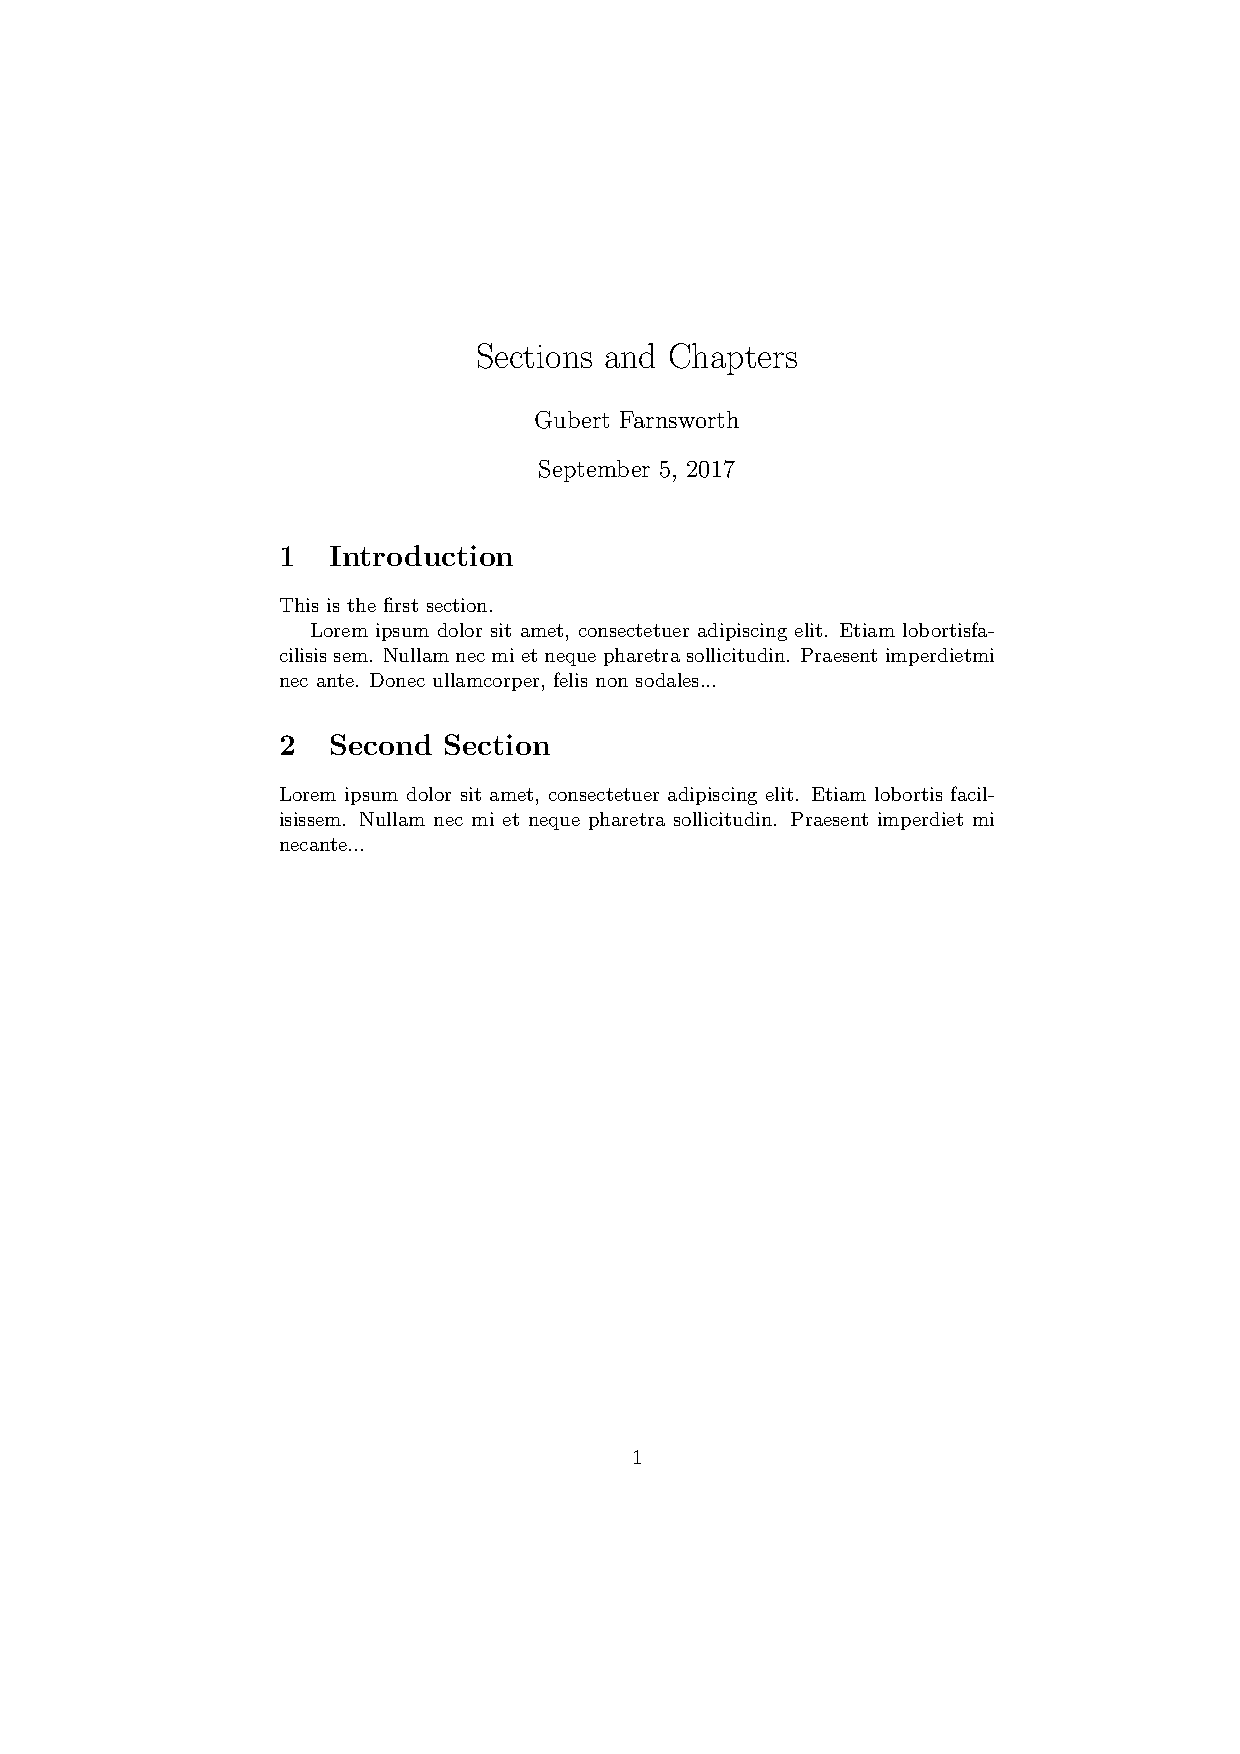
\includegraphics[scale=0.39]{./resources/figures/netl.png}
    \end{mdframed}
    \caption[nETL Architecture]{\textbf{Figure \ref{nETL}: nETL Architecture.} \textit{nETL} is an ETL framework designed to host user-created \textit{Modules} to define \textit{extraction}, \textit{transformation} and \textit{loading} processes. \textit{Modules}, shown in the colored boxes, consist of two parts: a configuration object (a JSON object) and a function that adheres to the specified contract. On startup the \textit{nETL} framework loads modules via the operations via a function made available by the main class. The modules are then cached in main memory by the \textit{nETL} process. A user can then interact with the TaskManager class to create a new task via loading a JSON configuration that makes use of a particular \textit{Module}. Tasks consist of an \textit{Extraction module} configuration, several \textit{Transformation module} configurations and a \textit{Load} configuration. Because modules are created and defined by users, as well as the order in which modules are executed, input/output contracts are also defined by the user, and as such \textit{ETL} processes are infinitely configurable.}
    \label{nETL}
\end{figure}
\section{Implementation}
The ETL engine and modules (extractions, transformations, loads) are implemented in JavaScript (\textit{ECMAScript 2017\textsuperscript{®}}) \cite{ecmascript2017} and designed to run in the context of the \textit{node.js} runtime environment \cite{nodejs}. \textit{node.js} emphasizes asynchronous input/output (IO), making it a good fit for handling ETL tasks in which IO (CouchDB is accessed exclusively via network requests) accounts for the greatest amount of computational overhead. Since \textit{node.js} runs server-side it provides access via JavaScript to the file system, which is required in terms of an ETL tool. JavaScript is a sensible language in which to implement nETL in the context of this project:

\begin{itemize}
    \item It has a very succinct API making it fast to write code in (i.e. it is a highly abstracted language similarly to Ruby or Python)
    \item But unlike Ruby or Python (and other high level languages), it is opinionated in that it handles IO asynchronously by default
    \item The JavaScript implementation of object-orientation is appealing (to some developers at least \cite{jsBook})
\end{itemize}

Modules are implemented via the \textit{revealing module} pattern, in which functions are returned from functions; parent functions create scoped execution environments that is similar in concept to instantiating classes\footnote{JavaScript has classes, but these are just syntactic sugar implemented partially via closure}. Compared to working with constructors closure provides more isolated scope. For each level of closure an additional scope is created that is available solely to functions defined within that scope. Figure \ref{fig-scope} shows code in which three scoped environments have been defined: a global scope, an Immediately Invoked Function Expression (IIFE) scope, and an \textit{exe}-function level scope (all of these are closed over by an \textit{invoke} function). JavaScript has \textit{lexical} scope \cite{jsBook2} that (for this purposes of this project) allows for configuring modules differently at different levels in object hierarchy without having to re instantiate modules that have already been loaded.

\begin{figure}[H]
  \centering
  \begin{mdframed}[rightline=true,leftline=true]
    \begin{minted}{text}
// Global scope

// Closure over the global scope
(function() {
    // Module-specific scope

    // Closure over module-specific scope
    function exe(configurationObj) {
        // Task-specific scope

        // Closure over task-specific scope
        function invoke() {...};

        return {
            invoke: invoke
        };
    };

    return {
        name: "MODULE_NAME",
        exe: exe
    };
})();
    \end{minted}
  \end{mdframed}
  \caption[Module Scope via closure]{\textbf{Figure \ref{fig-scope}: Scoping via closure in JavaScript}}
  \label{fig-scope}
\end{figure}

Modules are loaded into the nETL engine by invoking a function (an IIFE in terms of Figure \ref{fig-scope}) that returns an object with a \textit{name} property for identification and that references the \textit{exe} function. Loading many modules into the application results in a list of available module names, with each name in turn referencing a function named \textit{exe} (these are different functions with the same name). This is shown in Figure \ref{fig-module-memory} as the list with the heading \textit{Module Definitions}.

When a task specifies that a module should be used (identified by a name), A lookup for that name in the Module Definitions list is performed and the corresponding \textit{exe} function is executed. This returns a scoped execution context\cite{executionContext} in which another function called \textit{invoke} is required to be defined (nETL users author the body of the \textit{exe} function). The task assigns the name of the module to the \textit{invoke} function definition, which during task-execution may be called many times to perform extraction, transformation, or loading logic. A list of \textit{Loaded Modules} is maintained for each running task as shown in Figure \ref{fig-module-memory}. Each of the referenced functions maintains closure over the execution context created on \textit{exe} invocation, thus allowing for a module to be loaded once but configured for specific tasks; every time an \textit{exe} function is called a new closed scope is created only accessible to the callee.

\begin{figure}[H]
    \centering
    \begin{mdframed}
        \centering
        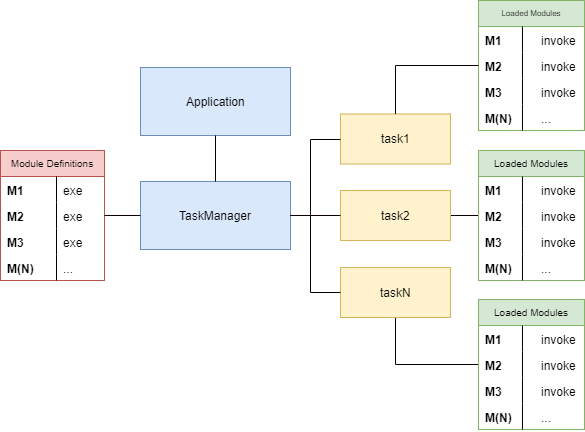
\includegraphics[scale=0.62]{./resources/figures/fig-module-memory.png}
    \end{mdframed}
    \caption[Loaded module representation]{\textbf{Figure \ref{fig-module-memory}: Loaded module representation}}
    \label{fig-module-memory}
\end{figure}

All modules adhere to the modular contract as shown in Figure \ref{fig-module-contract} such that invoking a module returns a \textit{Promise} \cite{jsPromises} that resolves an \textit{invoke} function. This function accepts a single parameter and returns a \textit{Promise} that resolves the result of the module (which differs depending on whether a module performs extraction, transformation or loading operations). JavaScript \textit{Promise} objects are state-representation of asynchronous operations in terms of success and failure of these operations. Since logic implemented in a module may not be asynchronous, all logic is wrapped within a \mintinline{text}{setImmediate} function to ensure that the contract of asynchronous execution of all modules is adhered to (except for where generators are used, since \textit{ECMAScript 2017\textsuperscript{®}} does not support asynchronous generator functions).

\begin{figure}[H]
  \centering
  \begin{mdframed}
    \centering
    \begin{minted}{text}
(function () {
    // Execution context ('this') is a config object
    function invoke(obj) {
        return new Promise((resolve, reject) => {
            setImmediate(() => {
                try { resolve(obj); }
                catch (error) { reject(error); };
            });
        });
    };
    return new Promise(async(resolve, reject) => {
        setImmediate(() => {
            try { resolve({ invoke: invoke }); }
            catch (error) { reject(error); };
        });
    });
})();
        \end{minted}
  \end{mdframed}
  \caption[nETL module contract]{\textbf{Figure \ref{fig-module-contract}: nETL module contract}}
  \label{fig-module-contract}
\end{figure}

On task execution (as directed by a user via the CLI) a task is run from beginning to end, iteratively extracting batches of data from a source, transforming that data, loading that data and then repeating the process. Since IO in JavaScript is asynchronous, batching either needs to be run sequentially (batches are processed one after the other), or by carefully managing asynchronous execution of batches. Batches extracted asynchronously and concurrently would quickly overwhelm the network capabilities of any computer since thousands of network requests would be queued instantaneously (network IO is many times slower than file IO, which is many times slower than data transformation). Most of these requests would fail - it is easier to serialize processing of batches than to queue network requests. As such, nETL is implemented to execute separate tasks concurrently; but a single task comprises a series of sequential steps.

JavaScript is not truly parallel - concurrent execution is achieved via adding procedures to an event loop that is executed on a first-in first-out basis via a single thread, with certain operations specified to be implemented asynchronously. Certain functions in JavaScript (\mintinline{text}{setTimout}, \mintinline{text}{setImmediate}, and \mintinline{text}{setInterval}) along with certain environment-provided APIs (such as the node.js filesystem API) pass control back to the event loop before execution of these functions is completed. Such operations allow for specifying a callback function that is added to the event queue at time later from when the asyncrhonous function is first called. So if two tasks are running concurrently and a blocking procedure is called that is not asynchronous, processing of the event queue would be paused until the blocking procedure is completed. As a result, both tasks would be blocked until the procedure completes and the next item on the event loop is processed.

For this reason each step in the ETL engine (extraction, transformation and loading) is implemented asynchronously. Prior to the ECMAScript 2017 specification, an ETL engine implemented in node.js would have been challenging and require complex state management of asynchronous operations. But via the \textit{async}/\textit{await} API (a wrapper for JavaScript \textit{Promises}), such state management is straightforward as shown in Figure \ref{fig-engine} \footnote{Actually the extraction operation (\mintinline{text}{batch = batch.next()}) is NOT awaited (the \mintinline{text}{next} function is not asynchronous) because asynchronous generators are not supported in ECMAScript 2017}.

\begin{figure}[H]
  \centering
  \begin{mdframed}[rightline=true,leftline=true]
    \begin{minted}{text}
while (!batch.done) {
    values = batch.value;
    payload = await values.reduce(async(previousResults, item) => {
        const results = await previousResults;
        await asyncForEach(transformations, async(t) => {
            item = await t.invoke.call(t, item);
        });
        if (item !== {} && item) results.push(item);
        return results;
    }, []);
    loadResult = await load.invoke(payload);
    batch = batches.next();
};
    \end{minted}
  \end{mdframed}
  \caption[Serializing asynchronous operations]{\textbf{Figure \ref{fig-engine}: Loop with serialized asynchronous operations}}
  \label{fig-engine}
\end{figure}

\subsection{Extracting data}
Files are read in 64KB chunks from beginning to end within the context of an iterator created by a JavaScript \textit{generator} function \cite{mozillaGenerators}. Chunks are held in memory, split into lines (identified by \textit{LF}, \textit{CR} or \textit{CRLF} line ending markers to allow for cross-platform portability) and yielded a single line at a time to a controlling function executed within the context of the iterative ETL engine. This function iteratively collects \mintinline{text}{n} lines at a time into a list (\mintinline{text}{n} is a user configurable property \textit{batchSize}) and yields ``lists of lines'' - (\textit{batches}). Generators are useful in the regard because they automatically create a state handling mechanism for iterating over file contents - i.e. pointers to positions in files, references to incomplete lines as retrieved from files, etc. Disk access via generators is achieved via code taken directly from an open-source library \cite{bower16}.

Lines in batches are then transformed concurrently, with transformations (specified in configuration) applied to each line in the batch in the order specified in the configuration. Concurrent processing of items accessed via a loop is achieved by wrapping the loop body in an asynchronous function (\mintinline{text}{setImmediate}), allowing the loop to progress without waiting for loop body execution to complete.

The loop itself is awaited, however, and once all transformation have been applied to all lines in the batch (lines can also be discarded from the batch depending on the transformations applied), the transformed batch is returned to \mintinline{text}{taskManager} and passed as an argument to the loading function specified via configuration. The function's contract is such that \textit{taskManager} is notified when the batch has been loaded successfully to the destination, at which a further batch of lines is generated and processed. This batching loop is repeated until the extraction generator returns false when the end of a data source is reached.

\subsection{Transforming data}
In terms of processing lines in a flatfile (CSV format), headers are only ever read once with the assumption that the all rows can be split into values (by some defined delimiter) and that the order of the values corresponds with the order of the headers - if this is not the case, then the CSV is malformed. A reference to the CSV header row that is maintained for the duration of the transformation. CSV rows are iteratively loaded into memory and split into values. Row values are matched with header values to form key:value pairs and create JavaScript objects

After transforming row-strings into row-objects, additional transformations are applied to each object. The following transformations are applied to objects:

\begin{itemize}
    \item \textbf{Selection-filter:} Entire objects can be whitelisted based on properties and allowed values for those properties.
    \item \textbf{Join-selection-filter:} A list of attributes and values can be retrieved from a \nth{3} party data source (for example from a CouchDB index), and entire objects can be whitelisted based on the retrieved attributes and allowable values for those attributes. This is similar in concept to a join, although no means of actually joining documents is provided (i.e. creating attributes based on data retrieved from a \nth{3} party data source instead of applying selection - although this would be a fairly easy feature to implement).
    \item \textbf{Projection-filter:} Unneeded attributes can be removed from objects prior to loading into database/other destinations
    \item \textbf{Projection-append-attributes:} Additional attributes can be added to objects - e.g. a \textit{type\_} attribute can be added, along with a value as specified by configuration
\end{itemize}

\subsection{Loading data}
Batches of objects are serialized to JSON and are loaded into a CouchDB database via the the HTTP POST \_bulk\_docs endpoint (as opposed to separate network requests for each item in a batch). Bulk inserts are configured to be atomic - i.e. either an entire insert succeeds or fails. Network requests make use of the well-known, open-source node.js library ``request'' \cite{request-lib}.
\section{Setup}
Running nETL requires an installation of node.js V8.9.0 +, which should include an installation of npm. After cloning the netl repository from Github to a local drive, dependencies should be restored using the npm CLI tool. Additionally, the directory \mintinline{text}{C:\log} needs to be created, and then the nETL app can be started from a terminal. Once the CLI is running, typing anything into the terminal and pressing enter outputs help where further direction can be obtained.

In conjunction with setting up nETL, a CouchDB server needs to be configured. This is easy to do on Windows machines - simply download the executable from apache.org and use the installer. Once installed the server should be run in single node configuration, binded to the 127.0.0.1 address. This allows access to the CouchDB UI via the browser at the address: \url{http://127.0.0.1:5984/\_utils}, where first an admin user should be created. Working with databases via the CouchDB interface (called Fauxton) is straightforward.

Database creation involves only the single step of specifying a name and (optionally) security roles. CouchDB database configuration should be specified as part of creation - though this is only available when databases creation is specified via the HTTP interface and not the Fauxton GUI (the UI doesn't allow for case-by case configration in this case, but does allow for global configuration changes - although this is not recommended \cite{fauxton}); examples of configurable settings are sharding (q) and replica (n) count. For a single node setup, q=8 and n=1, meaning that a database has 8 shards and only 1 replica of each shard. This is the configuration used in this project. There is no point in storing more than one copy of a single shard on a single server, which is why n=1. For CouchDBs operation in cluster mode the default setup is q=8 and n=3. For clusters with a large number of nodes it might make sense to increase the value of the q parameter.

\subsection{CouchDB Design Documents}
Design documents are simply JSON strings, in which JavaScript functions are defined as strings. Working directly in JSON is unpleasant, however, and as such a open source tool, ``couchapp'', written in Python is used for configuring and installing Design Documents to CouchDB databases \cite{pythonCouchapp}. This tool maps a directory structure to a JSON document; in other words, directory names become keys, and directory contents is reference by these keys as values in the JSON document. Directories can be nested in the same way that JSON allows nesting objects; nested directories translate to nested keys in the final JSON document.

Using this tool, Map and list functions are included as a single JavaScript files within the couchapp directory. Working with JavaScript files for Map and List functions provides the benefit of isolating the code (useful for unit testing) as well as benefits achieved from using an IDE - code completion, syntax highlighting, etc.

\chapter{Analysis}
\label{chapter-analysis}
CouchDB's MapReduce implementation is limiting in terms of performing \textit{joins} and \textit{selections} across multiple entities for a number of reasons:

\begin{itemize}
    \item Every document is processed during index calculation; limiting the size of the database footprint greatly improves performance as a result. This can be done by only including entities that are required for index output in a database.
    \item Indexes are derived from a single database (you cannot cross reference multiple databases from a map or reduce function)
    \item Although basic filtering can be performed within a Map function, filters cannot be dynamic and have to be hard coded. For example, it is not possible to write a map function that filters out documents on a field for values found in other documents/indexes in the database. The context in which map and reduce functions are executed is pure JavaScript, with no means of IO to either a file system or over network requests made available \cite{slack28Feb}. Execution of Map and Reduce functions is necessarily idempotent and for this reason, and for security reasons, database state cannot be altered from a map / reduce function during index calculation
\end{itemize}

With CouchDB's means of data retrieval seemingly crippled compared to SQL, it is necessary to keep in mind CouchDB's benefits (as discussed previously) compared to such databases to stay in good humor! In conjunction with external tools such as the nETL software, however, \textit{joins} and \textit{selections} can be implemented with relative ease.

\section{Joining Data}
The three datasets used in this project require joining on the StudentID field. This field appears once for every student in the benchmarks data, several times for each student in the grades data and up to thousands of times per student in the events data. Both the grade and event data contain a field for year - i.e. the year in which a grade was obtained or the year in which an event was registered. As such these two datasets require joining on both the StudentID and Year fields. Benchmark data is only collected once per student enrollment, and as such is associated with grade and event data only by StudentID. To describe the join in terms of SQL, an \textit{INNER JOIN} is performed on the grades/events data, and the resultant dataset is joined to benchmark data via a \textit{LEFT OUTER JOIN}.

Initially an attempt was made at joining the three entities directly via MapReduce; the map function in this case was configured to output identical keys across the three entities for rows that require joining, and tuple as a value in which index position indicates the value-output of specific entities. With the map function output a tuple of 11 indexes instantiated with null values (actually the value `0' to represent falsy numerical values), each index (or group of indices) is reserved for a specific entity type's output and adjusted appropriately during map function execution depending on the type of document the map function is applied to (the map function executes once for every document in the database):

\begin{minted}[linenos=false]{text}
[
   0,                          # i = 0: a course % grade or 0
   0, 0, 0, 0, 0, 0, 0, 0,     # 0 < i < 8: benchmark grade %s
   0, 0                        # 8 < i > 11: event count for semester 1/2
]
\end{minted}

Depending on the value of the `type\_' attribute of the document being processed by the map function, values at relevant indices of the tuple for that particular document type are altered to represent the info in the document that should be output. If the document being processed by the map function is of \textit{type\_} ‘grade’, then the map function emits a tuple with a value at \mintinline{text}{i = 0} and 0s for all other indices: \[[\%, 0, 0, 0, 0, 0, 0, 0, 0, 0, 0]\]

If the document is of \textit{type\_} `benchmark', the map function emits a tuple with values at \mintinline{text}{0 < i < 8}: \[[0, \%, \%, \%, \%, \%, \%, \%, \%, 0, 0]\]

If the document is of \textit{type\_} ‘event’, the map function emits a tuple with values at \mintinline{text}{8 < i > 11}: \[[0, 0, 0, 0, 0, 0, 0, 0, s1EventCount, s2EventCount]\]

Structuring tuple output, in terms of reserving indices for specific data representations allows for preserving separation of information by document \textit{type\_} even when tuples are processed without context provided by the \textit{type\_}, \textit{StudentID}, \textit{CourseCode} or \textit{Year} attributes - these are removed by the map function; tuples are grouped by common key as output by the map function and passed to the reduce function as a list of tuples per key. The join is performed during execution of the reduce function (in addition to aggregating event document of a single student in a single year into a single document).

The reduce function is passed key:value pairs, where unique keys are associated with a list of tuples; together, these tuples represent information of all three entities, and since they are all passed to a single reduce function a join is achievable (the reduce function is effectively able to process information from all three entities for a single key). The key in this case is compound, and has the form:

\[[StudentId,CourseCode,Year]\]

But the Events data doesn't include Course, and the the Benchmarks data doesn't include Course or Course Year. As such, to allow for Grade data to be joined to Benchmark data on Course and Course Year in addition to Student ID, each Benchmark document needs to be output for every possible combination of Course and Course Year per student. That is the same with the Events documents - each Event needs to be output for every possible course that a student took in a given year.

In terms of performance this approach is disastrous. To analyze 40 courses taken over 3 years, each Benchmark document needs to be emitted for a student $40 x 3 = 120$ times so that the key of the Grade document [Student ID, Course, Year] can always be joined to Benchmark document. Likewise, Each Event data (which has year but not course information) needs to be emitted 40 times - once for each course a join could potentially be performed on. Considering the large number of event documents, this is impracticable. For this approach to be efficient, event documents would need to be aggregated prior to joining to minimize the number of times event data is replicated.

Instead, CouchDB's usage of B+trees as a means of sorting view indexes by keys is utilized to allow for joining the 3 documents in the final dataset. Figure \ref{fig-mapreduce-key-output} shows key output for all three entities in the form: [ID, Course, Year]. Documents that don't have properties for these fields emit 0 instead; resulting in a predictable key format of for each entity that is ordered:

\begin{itemize}
    \item \textit{benchmarks} document: [Id, 0, 0]
    \item \textit{events} document: [Id, 0, Year]
    \item \textit{grades} document: [ID, Course, Year]
    \item \textit{grades} document: [ID, Course, Year]
    \item etc...
\end{itemize}

Although many \textit{events} documents are outputted by the map function per student, due to reduction grouping all these documents by common key, only a single document that is an aggregation of all \textit{events} documents will be stored as reduced output in the view. So, for any student ID, scanning the index iteratively produces first a Benchmark document, then a single (aggregated) Event document, then a single Grade document for each course that student enrolled in. Because output is systematically processed a student at a time, with grades, events and benchmark data iteratively process in a predictable order per student, joins can be achieved by holding documents for a particular StudentID in memory and processing grades, events, benchmarks for that StudentID. When a new StudentID is encountered, a joined row is output, memory is flushed and a new joined row for the new studentID is started. This results in a much more efficient way of aggregating/joining different types of documents for a given set of keys.

\begin{figure}[H]
    \centering
    \begin{mdframed}
        \centering
        \begin{minted}{text}
// Map output
[<ID>, ‘0’, 1]: [0, b1, b2, b3, b4, b5, b6, b7, b8, 0, 0]
[<ID>, ‘0’, <Year>]: [0, 0, 0, 0, 0, 0, 0, 0, 0, 1, 0]
[<ID>, ‘0’, <Year>]: [0, 0, 0, 0, 0, 0, 0, 0, 0, 1, 0]
[<ID>, ‘0’, <Year>]: [0, 0, 0, 0, 0, 0, 0, 0, 0, 0, 1]
[<ID>, ‘0’, <Year>]: [0, 0, 0, 0, 0, 0, 0, 0, 0, 0, 1]
[<ID>, ‘0’, <Year>]: [0, 0, 0, 0, 0, 0, 0, 0, 0, 0, 1]
[<ID>, ‘0’, <Year>]: [0, 0, 0, 0, 0, 0, 0, 0, 0, 1, 0]
[<ID>, ‘CSC1015F’, <Year>]: [98, 0, 0, 0, 0, 0, 0, 0, 0, 0, 0]
[<ID>, ‘MAM100F, <Year>]: [94, 0, 0, 0, 0, 0, 0, 0, 0, 0, 0]

// Resulting reduce output
[<ID>, ‘0’, 1]: [0, b1, b2, b3, b4, b5, b6, b7, b8, 0, 0]
[<ID>, ‘0’, <Year>]: [0, 0, 0, 0, 0, 0, 0, 0, 0, 3, 3]
[<ID>, ‘CSC1015F’, <Year>]: [98, 0, 0, 0, 0, 0, 0, 0, 0, 0, 0]
[<ID>, ‘MAM100F, <Year>]: [94, 0, 0, 0, 0, 0, 0, 0, 0, 0, 0]
        \end{minted}
    \end{mdframed}
    \caption[Aggregation By Sorted MapReduce output]{\textbf{Figure \ref{fig-mapreduce-key-output}: \textit{map} and \textit{reduce} function output}
    \label{fig-mapreduce-key-output}
\end{figure}


\section{Selecting Data}
Performing joins via iterating over ordered indices is quite efficient in terms of memory usage. No matter the size of datasets being processed, memory usage will always be fairly low. An increase in size of datasets will simply result in more processing time. Selections performed during the MapReduce stage are therefore completely feasible regardless of the size of the dataset being queried. However, in terms of time, selections are expensive when performed as part of the MapReduce process; the events data as over 40 million records of which a very small number are selected for this analysis. To perform a selection on the events data during MapReduce requires iterating through through all events records - which is expensive in terms of time.

Additionally, it is impossible to select records by a field in which values are specified dynamically. This means that selecting data during MapReduce requires an additional step in data-analysis in which a list of values to use for filtering are determined either via using an additional CouchDB view, Microsoft Excel, a SQL database, etc. CouchDB's MapReduce engine doesn't allow any database, file, etc. interactions by design, and although it's possible to swap out the default MapReduce engine with one that does allow this, this is not recommended. An experiment to implement the couchjs engine using Google's V8 engine (i.e. using node.js) is available on online \cite{v8couchjs}, which is misleading since that is the JavaScript implementation that \textit{node.js} uses. Replacing the default couchjs engine with this one, it would seem as if network requests from map function execution should be possible (making dynamic filtering possible). However, this experiment was abandoned in 2013 precisely because it is too difficult to disable the numerous APIs that the V8 engine makes available to runtime JavaScript code. The CouchDB specification is that the MapReduce execution environment is required to be isolated in terms of interactions with the database or other instances of MapReduce function execution for security and to maintain integrity of the data layer \cite{slack28Feb}.

Primarily for this reason, selection is implemented during the ETL phase of the analysis in nETL. A dynamic filter is used as part of the transformations pipeline, in which a URI to a CouchDB view is specified. The result of this view is used to filter (i.e. perform selection) on data extracted from the CSVs, with only relevant rows from the CSV added to the database. This approach requires configuring an additional index prior to loading data into the database.

This project requires filtering events/benchmark data by students who attended the CSC1015F course. Dynamic selection (i.e. selection via fields using a \textit{JOIN} statement) is implemented via the following workflow:

\begin{itemize}
    \item A CouchDB database of grade documents is created with an index of student IDs for which a grade is available for the CSC1015F course
    \item During ETL, the index of the grades database is retrieved, and rows of events/benchmarks data are filtered according to student numbers as retrieved in the index
    \item Remaining rows after filtering are then loaded into CouchDB where they are indexed, and joined on retrieval
\end{itemize}

\section{Analysis Workflow}
Although the MapReduce function fills the important role of aggregating entities prior to joining them (as discussed in 3-way join section), it is technically possible to join documents directly on retrieval from the main database file since both the main database file and derived indexes are structured as B+trees and can be sorted. However there are three problems with retrieving data directly from the main database file and skipping index creation:

\begin{itemize}
    \item CouchDB database files are sorted by the ``\_id'' field, which when unspecified on document insert is initialized as a UUID. Using UUIDs as unique document identifiers allow for distributed systems in which cluster nodes can operate independently of each other without the possibility of documents being created in separate nodes with conflicting IDs. Even though not required by this project, such best practices are followed. A B+tree sorted by a UUID is not useful for document retrieval, and as such, views are required of the underlying data store for any kind of index-based querying
    \item List functions are invoked via an HTTP GET request with the requirement of specifying a view within the URI. List functions are convenient for usage in this project as they facilitate ordered, iterative, range-based access (meaning that datum can be accessed sequentially, in isolation and in reliable order)
    \item When aggregations of specific entities are required, retrieving data directly from these indexes is vastly easier than having to aggregate during data retrieval. As aggregation logic becomes more complicated the difficulty of such direct data retrieval increases and the benefit of using indexes increases as a result
\end{itemize}

As such, in terms of retrieving processed datasets useful for analysis, for each analysis the nETL and CouchDB applications are incorporated into an workflow represented by the following steps:

\begin{itemize}
    \item CSVs are parsed, rows filtered (selection) and data loaded into CouchDB by the nETL application
    \item An index is created from the CouchDB database via MapReduce
    \item Data is retrieved directly from the index file using a List function, during which time any required joining is performed
\end{itemize}

In terms of the MapReduce tasks, only built-in reduce functions are used; these functions (\_sum, \_count and \_stats) are implemented within the main Erlang process. This offers a performance boost over custom reduce functions since the IO transfer cost between the Erlang process and the view engine (couchjs.exe by default) is avoided. Working on a Windows machine, the IO cost is apparently exaggerated due to the difference between Unix-based and Windows kernel implementations \cite{slack1Nov}.

During analysis, runtime results of the different components of the system are recorded and are shown in Table \ref{performance-analysis}. The metrics include running time of nETL tasks, a summary of the data processed by nETL, CouchDB indexing times, and database/index storage footprints.
\section{2-Way Join}
An initial analysis computing the correlation between CSC1015F Grade and each Benchmark attribute requires a 2-way join between the Grades and Benchmarks datasets. To achieve this, two nETL tasks were run to extract the CSV data (the ``Grades.CSV'' and ``Benchmarks.CSV'' files) and load rows from these CSV files into CouchDB as documents of type ``grade'' and ``benchmark'' respectively. The JSON configuration file in which both these tasks are defined is included in the appendix at \ref{netl-tasks-1-2-config}. Following loading the data from the CSVs into CouchDB, a Map function is used to produce an index of the CouchDB documents ordered by Student ID, with the guarantee that for every unique student id documents are ordered by type; the demographic document preseeds the Grade documents for any given student. Knowing the order of documents via the view-index allows for performing the join on data-retrieval. For this analysis, retrieval (and joining) is performed via a CouchDB List function (discussed below), with the output in CSV format. Excel can then be used to compute correlations of this result.

\subsection{nETL Configuration}
The ETL processing of Benchmark data involves an iterative approach of first reading a batch of 10 000 lines from the CSV, performing transformations on each line in the batch, and then loading each batch into CouchDB. On notification that a single batch is loaded successfully into CouchDB, a further 10 000 lines are read from the CSV and processed in the same way. This process continues until the entire CSV has been read and loaded into CouchDB. Batches are loaded into CouchDB via the \textit{\_bulk\_docs}. A list of the transformations applied to each line extracted from each CSV is shown below:

\subsubsection{Task 1 Transformations (Grades)}
\begin{enumerate}
  \item A line is converted into a JavaScript object (which relates directly to the JSON format of CouchDB documents) with the fields:
        \begin{itemize}
          \item DownloadedDate
          \item RegAcadYear
          \item RegTerm
          \item anonIDnew
          \item RegProgram
          \item RegCareer
          \item Degree
          \item DegreeDescr
          \item Subject
          \item Catalog.
          \item Course
          \item CourseSuffix
          \item Session
          \item Percent
          \item Symbol
          \item UnitsTaken
          \item CourseID
          \item CourseDescr
          \item CourseCareer
          \item Faculty
          \item Dept
          \item MaximumCrseUnits
          \item CourseCount
          \item CourseLevel
          \item CESM
          \item Sub-CESM
        \end{itemize}
  \item Lines (now in object form) are filtered on the ``RegCareer'' and ``Course'' fields, where grades achieved for the CSC1015F course taken by students registered as undergrads are considered. Lines that don't meet this attribute are discarded and no further transformations are applied to these line
  \item An attribute (``type\_'') is then added to each line (that weren't removed in filtering step), and given the value ``grade'' to identify each object as a line of the Grade entity type
  \item Document attributes are whitelisted. The resultant documents each have the the following attributes:
        \begin{itemize}
          \item type\_
          \item Course
          \item RegAcadYear
          \item anonIDnew
          \item Percent
        \end{itemize}
\end{enumerate}

\subsubsection{Task 2 Transformations (Benchmarks)}
\begin{enumerate}
  \item A line is converted into a JavaScript object with the fields:
        \begin{itemize}
          \item anonIDnew
          \item Career
          \item Citizenship Residency
          \item SA School
          \item Eng Grd12 Fin Rslt
          \item Math Grd12 Fin Rslt
          \item Mth Lit Grd12 Fin Rslt
          \item Adv Mth Grd12 Fin Rslt
          \item Phy Sci Grd12 Fin Rslt
          \item NBT AL Score
          \item NBT QL Score
          \item NBT Math Score
          \item RegAcadYear
        \end{itemize}
  \item Lines are filtered on the ``Career'', ``Citizenship Residency'', and ``anonIDnew'' fields. Only lines for students that attended the CSC1015F course during their undergraduate career and that are either South African citizens or permanent residents are included in the result set. The list of students that attended CSC1015 is derived from the Grade data
  \item An attribute (``type\_'') is then added to each remaining line and given the value ``benchmark'' to identify each object as a line of the Benchmark entity type
  \item Attributes are whitelisted. The resultant documents each have the the following attributes:
        \begin{itemize}
          \item type\_
          \item anonIDnew
          \item Eng Grd12 Fin Rslt
          \item Math Grd12 Fin Rslt
          \item Mth Lit Grd12 Fin Rslt
          \item Adv Mth Grd12 Fin Rslt
          \item Phy Sci Grd12 Fin Rslt
          \item NBT AL Score
          \item NBT QL Score
          \item NBT Math Score
          \item RegAcadYear
        \end{itemize}
\end{enumerate}

\subsection{Map Function}
The map function for this analysis is included in the appendix (see \ref{2-way-join-map-function}). Each document passed to the map function is treated according to the logic shown in the activity diagram in Figure \ref{2-way-join-map-fn-diagram}. That is, on Map function execution the ``type\_'' attribute is checked. If the document is a line of the Grades entity, then the key [Student ID, Course, year] is emitted along with a single number for the value - the percent achieved for the course. If the document is a line of the Benchmarks entity, then the key [student ID, 0, 0] is emitted along with an ordered list of 8 values corresponding to values for the fields in the Benchmarks.CSV file:

\begin{itemize}
  \item Gr12 English \%
  \item Gr12 science \%
  \item Gr12 Math \%
  \item Gr 12 Math Lit \%
  \item Gr12 Adv Math \%
  \item NBT AL \%
  \item NBT QL \%
  \item NBT Math \%
\end{itemize}

Normalization of the percentage fields (i.e. ``Percent'' for the Grades entity and the test results in the Benchmarks entity) is done via a nested function within the Map function as discussed previously (Table \ref{tbl-grades-normalize} and Table \ref{tbl-benchmarks-normalize}). No reduce function is used to achieve this 2-way join. This is because, theoretically, a student should only have a single set of Benchmark results and should only achieve a single grade per course per year. As such there is no need to aggregate output from the Map function (which is done via reduction) before performing the document join via the List function.

\begin{figure}[H]
    \centering
    \begin{mdframed}
        \centering
        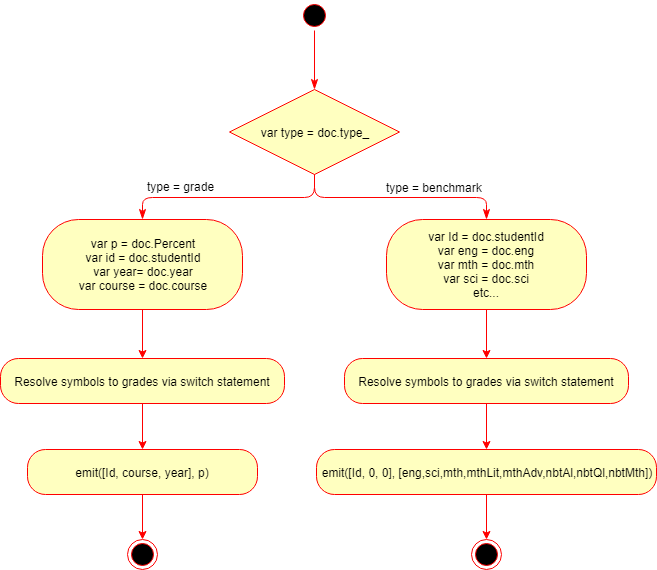
\includegraphics[scale=0.59]{./resources/figures/2-way-join-map.png}
    \end{mdframed}
    \caption[2-Way Join Map Function]{\textbf{Figure \ref{fig-2-way-join-map-function}: 2-way join \textit{map} function logic}
    \label{fig-2-way-join-map-function}
\end{figure}


\subsection{List Function}
The list function is executed via a call to CouchDB's HTTP API. For the project the URI of that function call is \url{https://localhost:5984/msc/\_design/2-way-join/\_list/2-way-join-list/ 2-way-join-view?reduce=false}. On invocation the List function opens and scans the index iteratively processing each document (i.e. iteratively processing each student; first a student's demographic document is processed, then a student's grades documents are processed).

Figure \ref{fig-2-way-join-list-function} shows an activity digram representing the logic used to perform the 2-way join in the List function. The logic is wrapped in a CouchDB helper function \mintinline{text}{provides()} that accepts two arguments: the type of data the list function will emit (CSV - i.e. plain text data), and a callback that allows uses to create the data that is transformed to the output type. Within the body of the callback the variables `currentStudent', `currentYear', and `currentLine' are set to null. An iteration over the index is initiated using a while loop, with the loop invariant the result of a call to the \textit{getRow()} function. When a row exists, a check is performed on whether the Student ID of the current row is the same as the Student ID of the previous row. If not, the currentLine variable is emitted via the \textit{send()} function, and currentStudent is adjusted to be the Student ID from the current row. Then the type of row being processed is checked (i.e. whether this key:value pair was emitted from a grade or benchmark document). If from a benchmark document, the scores are added to the currentLine variable and the loop re-executes. If a Grade document, there is a check as to whether \textit{currentYear} has the same value as the Year property in the current row. If not, the \textit{currentLine} variable is emitted and \textit{currentYear} is adjusted to the new Year value and the loop re-executes. When the loop invariant becomes false the subroutine to send the currentLine is executed one last time to take into account the last document processed.

\textit{currentLine} is emitted via a subroutine which first checks that the currentLine variable contains data from both the Grades and Benchmarks entity, and if not the line is discarded. Otherwise \textit{send()} is called with a comma-delimited string as a parameter, and this is emitted as output via a stay-alive network request (the connection is handled by the HTTP client). Code for the loop function is included in the appendix at \ref{2-way-join-list-function}.

\begin{figure}[H]
    \centering
    \begin{mdframed}
        \centering
        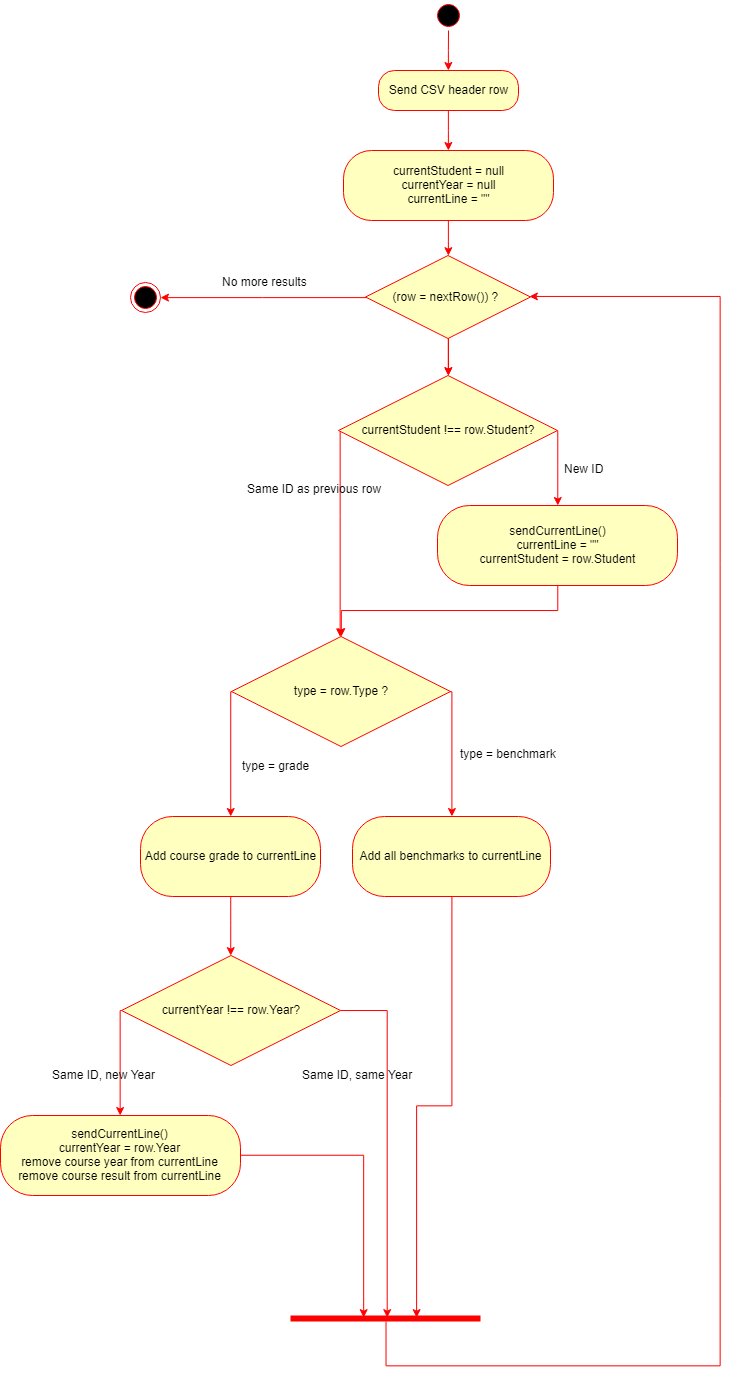
\includegraphics[scale=0.5]{./resources/figures/2-way-join-list.png}
    \end{mdframed}
    \caption[2-Way Join List Function]{\textbf{Figure \ref{fig-2-way-join-list-function}: List function logic required to join the Grades and Benchmarks entities.} Activity diagram of the code executed within the callback passed to the provides function executed by CouchDB during runtime of List function.}
    \label{fig-2-way-join-list-function}
\end{figure}


\subsection{Output}
A sample of the resultant joined dataset is shown in Figure \ref{fig-2-way-csv-output}. The full output has 1391 rows; 350 rows for the 2014 year, 457 rows for the 2015 year, 586 rows for the 2016 year. Many student IDs are repeated for different years; this occurs when students retake the course in a subsequent year. In this case, due to the nature of the sorted view index from CouchDB, all a student's course attempts are seen as separate, sequential rows in the joined output.

\begin{sidewaysfigure}
    \centering
    \begin{mdframed}[rightline=false,topline=false,leftline=false]
        \centering
        \begin{BVerbatim}
+------+---------+----------+-------+---------+---------+---------+-------------+-------------+-------+-------+--------+
| Year |   ID    |  Course  | Grade | G12 Eng | G12 Sci | G12 Mth | G12 Mth Lit | G12 Mth Adv | NBTAL | NBTQL | NBTMth |
+------+---------+----------+-------+---------+---------+---------+-------------+-------------+-------+-------+--------+
| 2015 | 2749802 | CSC1015F |    71 |      79 |      72 |      85 |           0 |           0 |    86 |    94 |     91 |
| 2015 | 2794606 | CSC1015F |    77 |      75 |      84 |      78 |           0 |           0 |     0 |     0 |      0 |
| 2014 | 2854832 | CSC1015F |    87 |      88 |       0 |      97 |           0 |           0 |    81 |    83 |     82 |
| 2014 | 2860166 | CSC1015F |    37 |       0 |       0 |       0 |           0 |           0 |     0 |     0 |      0 |
| 2016 | 2862568 | CSC1015F |    63 |      80 |       0 |      95 |           0 |           0 |    78 |    79 |     82 |
| 2014 | 2863288 | CSC1015F |    81 |      86 |       0 |      93 |           0 |           0 |    82 |    86 |     90 |
| 2015 | 2863336 | CSC1015F |    66 |      71 |      74 |      75 |           0 |           0 |    76 |    78 |     66 |
| 2015 | 2864266 | CSC1015F |    49 |      55 |       0 |      74 |           0 |           0 |    59 |    66 |     61 |
| 2016 | 2864266 | CSC1015F |    64 |      55 |       0 |      74 |           0 |           0 |    59 |    66 |     61 |
| 2014 | 2880284 | CSC1015F |    64 |      68 |       0 |      93 |           0 |           0 |    65 |    92 |     78 |
| 2014 | 2881364 | CSC1015F |    68 |      87 |       0 |      84 |           0 |           0 |    81 |    86 |     73 |
| 2014 | 2882706 | CSC1015F |    85 |      82 |       0 |      97 |           0 |           0 |    83 |    83 |     92 |
| 2014 | 2890964 | CSC1015F |    80 |      74 |       0 |      88 |           0 |           0 |    78 |    88 |     71 |
| 2014 | 2894402 | CSC1015F |    78 |      70 |       0 |      86 |           0 |           0 |    66 |    71 |     70 |
| 2014 | 2894954 | CSC1015F |    87 |      72 |       0 |      94 |           0 |           0 |    81 |    93 |     88 |
| 2014 | 2895244 | CSC1015F |    64 |      77 |       0 |      85 |           0 |           0 |    72 |    54 |     45 |
| 2015 | 2896964 | CSC1015F |    76 |      77 |       0 |      84 |           0 |           0 |    66 |    82 |     71 |
+------+---------+----------+-------+---------+---------+---------+-------------+-------------+-------+-------+--------+
        \end{BVerbatim}
    \end{mdframed}
    \caption[Sample of 2-way CSV output]{\textbf{Figure \ref{fig-2-way-csv-output}: Sample of the 2-way join output CSV.} List function output is a CSV download with the schema as represented in this figure. The full CSV has 1391 rows; 350 rows for the 2014 year, 457 rows for the 2015 year, 586 rows for the 2016 year. Many student IDs are repeated for different years; this occurs when students retake the course in a subsequent year. In this case, due to the nature of the sorted view index from CouchDB, all a student's course attempts are sequential rows.}
    \label{fig-2-way-csv-output}
\end{sidewaysfigure}

\section{3-Way Join}
Building on the correlation analysis between course grades and benchmarks for CSC1015F, additional information concerning each student's Sakai usage is taken into account. Along with the ``Grades.CSV'' and ``Benchmarks.CSV'' files, a 3rd CSV ``Events.CSV'' is loaded into CouchDB via the nETL application. Since a single student may be associated with many rows in the Event data (sometimes even thousands of rows), a reduce function is used within the MapReduce job to aggregate the Events rows into a single document that is a count of Sakai presence events for first and second semester, with the output of this aggregation (and also the documents for the Grade and Benchmark entities) saved as a view, again, sorted by StudentID. Similarly to the 2-Way analysis of CSC1015F Grade/Benchmarks correlation, a CouchDB List function is used for retrieving data from the view index and performing the 3-way join.

In other words, this analysis addresses the question of whether making more frequent use of the Sakai platform is shown to increase course performance for CSC1015F, as well as looking at the correlation between benchmarking scores and LMS usage. However, the Events cannot be associated with particular courses for the purposes of this study since the Events data FK to course ID, is strictly relevant to the Sakai system only; the grades data has not been exported directly from the Sakai platform and the id that is referenced by Sakai events is not present in the dataset used. As such, this analysis takes into account only ``general usage'' of the Sakai LMS, and not usage of Sakai for these particular courses.

\subsection{nETL Configuration}
nETL Tasks 1 and 2 are the same as run previously for the 2-Way join, except that only course grades from 2016 are used (since the Events exports is only from 2016). The 3-Way join introduces a 3rd task - Task 5 - in which lines from the ``Events.CSV'' file are extracted, transformed and loaded into CouchDB using the nETL application. Tasks 3, 4 \& 5 as JSON configuration files are included in the appendix at \ref{netl-tasks-3-4-5-config}.

Using nETL, Task 5 execution comprises an iterative extraction of 30 000 lines at a time. Each line from each batch undergoes a series of transformations before the entire batch is loaded into CoucDB via the \textit{\_bulk\_docs} endpoint, following which, the iterative extraction continues. A list of the transformations applied to each line extract from the ``Events.CSV'' file by nETL is shown below:

\subsubsection{Task 5 Transformations (Events)}
\begin{enumerate}
  \item A line is converted into a JavaScript object (which relates directly to the JSON format of CouchDB documents) with the fields:
        \begin{itemize}
          \item event\_date
          \item event\_id
          \item uct\_id
          \item site\_key
          \item ref
        \end{itemize}
  \item Lines are filtered on the ``uct\_id'' and ``event\_id'' fields; only events with an event type of ``presence'' (event\_id = 282) for students enrolled in CSC1015F in 2016 are considered.
  \item An attribute (``type\_'') is then added to each line (that weren't removed in filtering step), and given the value ``event'' to identify each object as a line of the Event entity type.
  \item Line attributes are whitelisted. The resultant lines each have the the following attributes:
        \begin{itemize}
          \item type\_
          \item event\_date
          \item event\_id
          \item uct\_id
          \item site\_key
        \end{itemize}
\end{enumerate}

\subsection{MapReduce Functions}
The map function for this analysis is included in the appendix (see \ref{3-way-join-map-function}). Each document passed to the map function is treated according to the logic shown in the activity diagram in Figure \ref{fig-3-way-join-map-function}. Logical handling of the Grade and Benchmark entities is discussed previously.If the document is a line of the Events entity then the date of the event is categorized as either having occurred in semester 1 or semester 2. A key of [Student ID, 0, Year] is emitted along with the value (a 2-index tuple) of [S1, S2]. The S1, and S2 variables are 0 by default, and depending on the date of the presence event, one of these variables is altered to be `1'.

Using the \_sum reduce function, an aggregation is done across all documents with the same key; this means that per a student, an aggregation is performed on a single Grade document, a single Benchmark document, and many Events documents in which the S1 and S2 variables are summed to form the tuple [sum of S1, sum of S2]. Because of the key output of each type of entity, the resulting view-index is ordered by StudentID; for each StudentID documents are ordered by the second index in the key output (course), which means that Benchmarks and Events entities are sorted to be before grades for a student; and sorting via the 3rd index of each key results in benchmark data always being sorted to be before Events documents. As such, during view-index retrieval it can be taken as given that for a single student ID, first documents of type Benchmark will be retrieved, followed by documents of type Event, followed by documents of type Grade.

\begin{sidewaysfigure}
    \centering
    \begin{mdframed}
        \centering
        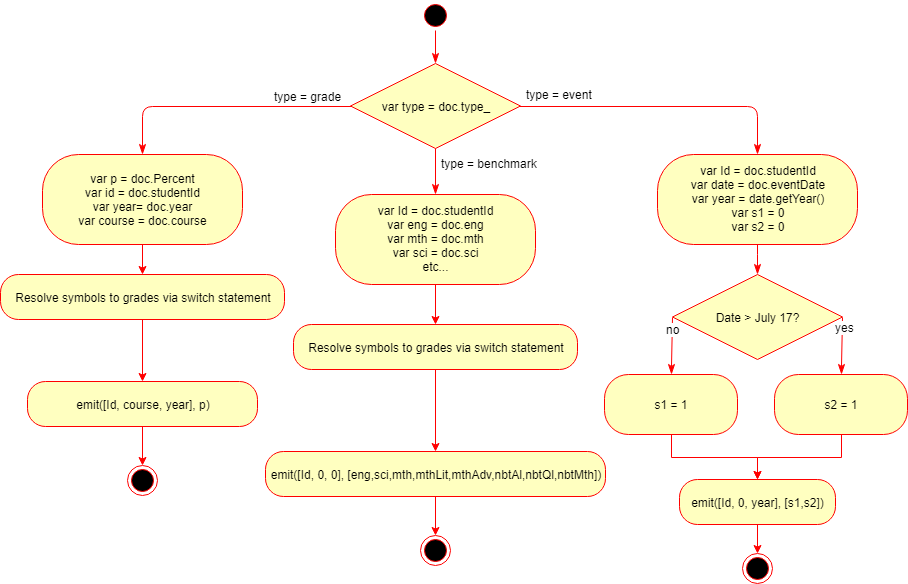
\includegraphics[scale=0.7]{./resources/figures/3-way-join-map.png}
    \end{mdframed}
    \caption[2-Way Join Map Function]{\textbf{Figure \ref{fig-3-way-join-map-function}: 3-way join \textit{map} function logic}}
    \label{fig-3-way-join-map-function}
\end{sidewaysfigure}


\subsection{List Function}
The List function is invoked via an HTTP request to the URI: \texttt{https://localhost:5984/msc /\_design/3-way-join/\_list/3-way-join-list/3-way-join-view?reduce=true}. On execution the list function executes the ``provides'' function, in which output type of ``CSV'' (plain text) is specified as as download file. List function logic as shown in Figure \ref{fig-3-way-join-list-function} is executed in the callback passed as a parameter to the ``provides'' function.

On initial invocation and within the body of the callback, the variables `currentStudent', `currentYear', and `currentLine' are set to null. Following this an iteration over the index is initiated within a while loop with the loop invariant the result of a call to the ``getRow'' function. While the loop invariant remains true (i.e. so long as the ``getRow'' function returns a row and not `false', which occurs after the last row has been retrieved from the index), a row - a reduced result - is processed (in the URI the parameter ``reduce'' is set to true, so ONLY reduced output is retrieved from the view). Similarly to List function logic for the 2-way join, after the loop invariant becomes false the last line is still in memory and is sent if necessary.

For every result retrieved from the reduce output , the StudentID of the row being processed is checked and compared to the StudentID of the previous row. If the current StudentID is not the same as the previous StudentID, a line of the CSV is emitted before the row is processed. Then, the type of result being processed is checked (either the document is of type ``benchmark'', ``event'' or ``grade''), and depending on the type different values are stored in a variable called ``currentLine''. For every StudentID, all types of documents are processed in turn (first the benchmark documents, then the event documents, then the grade documents) before being emitted. This allows the join to be performed via sequentially adding to the ``currentLine'' variable for a single student.

As as result of the MapReduce function, for every StudentID, exactly one ``benchmark'' result and one ``event'' document is processed. But a student can have several ``grade'' documents if the course was repeated in subsequent years. To catch this case, when processing documents of type ``grade'' within the switch statement, a further check is done to see if the attribute `year' of the current row has already been processed and is different from a preceding row. If so, the ``currentLine'' is emitted and the fields relating to grade documents are reset, and then repopulated with values from the current row (``currentLine'' itself is not reset). For every Event row processed both the first and second semester event count are exported to the CSV despite that only the first semester events are used, since there is negligible performance cost in terms of processing time or storage space and so there is little incentive to discard good data.

Conceptually, sending ``currentLine'' involves a call to a helper function provided within the execution context of CouchDB List functions - the ``send'' function. This function is wrapped within a subroutine (a function nested within the callback) that first checks that the currentLine variable contains data from the Grades and Benchmarks and Events entity, and then sends a comma-delimited string along a stay-alive network request - this is handled automatically by the HTTP client, which in the case of this project is simply the Google Chrome browser. From a user's perspective, it appears that a file is simply being downloaded; the rate at which the file downloads is equal to the rate at which the loop data is output by the send function. The download completes on completion of the List function. Code for the loop function is included in the appendix at \ref{3-way-join-list-function}.

\begin{figure}[H]
    \centering
    \begin{mdframed}
        \centering
        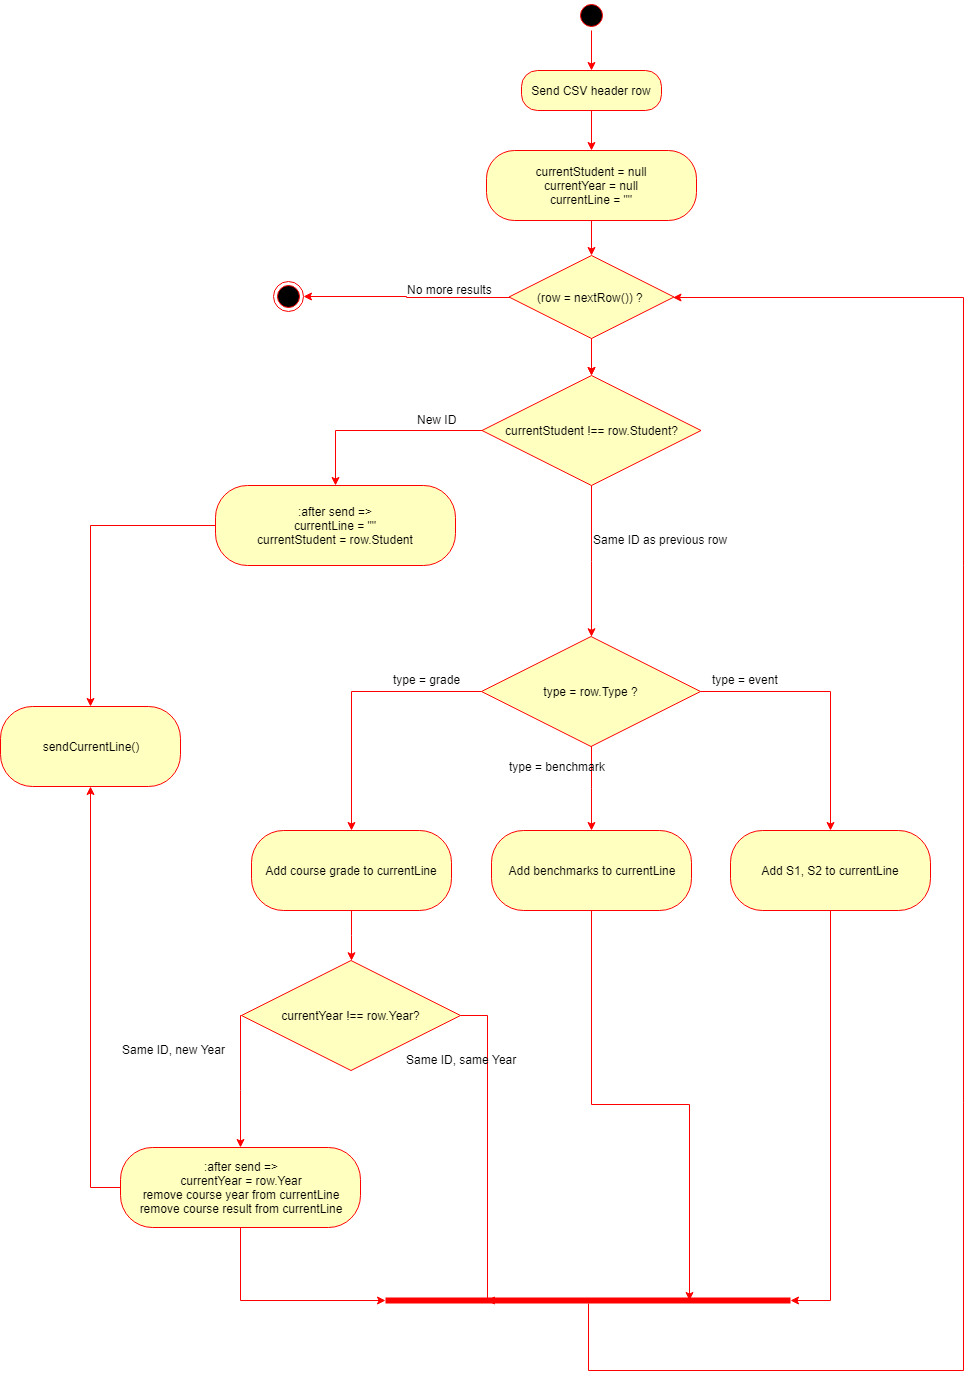
\includegraphics[scale=0.4]{./resources/figures/3-way-join-list.png}
    \end{mdframed}
    \caption[3-Way Join List Function]{\textbf{Figure \ref{fig-3-way-join-list-function}: 3-way join \textit{list} function logic}}
    \label{fig-3-way-join-list-function}
\end{figure}


\subsection{Output}
A sample of the resultant joined dataset is shown in Figure \ref{fig-3-way-csv-output}
\begin{sidewaysfigure}
    \centering
    \begin{mdframed}[rightline=false,leftline=false,topline=false]
        \centering
        \begin{BVerbatim}
+------+---------+----------+-------+----------+----------+----------+--------------+--------------+--------+--------+---------+------+------+
| Year |   ID    |  Course  | Grade | Gr12 Eng | Gr12 Sci | Gr12 Mth | Gr12 Mth Lit | Gr12 Mth Adv | NBT AL | NBT QL | NBT Mth |  S1  |  S2  |
+------+---------+----------+-------+----------+----------+----------+--------------+--------------+--------+--------+---------+------+------+
| 2016 | 2862568 | CSC1015F |    63 |       80 |        0 |       95 |            0 |            0 |     78 |     79 |      82 |  330 |  138 |
| 2016 | 2864266 | CSC1015F |    64 |       55 |        0 |       74 |            0 |            0 |     59 |     66 |      61 |  557 |  620 |
| 2016 | 2924430 | CSC1015F |    56 |       69 |       94 |       96 |            0 |            0 |     49 |     64 |      77 |  550 |  306 |
| 2016 | 2925212 | CSC1015F |    60 |       76 |        0 |       77 |            0 |            0 |     69 |     84 |      73 |  124 |  155 |
| 2016 | 2928032 | CSC1015F |    30 |       76 |        0 |       73 |            0 |            0 |     85 |     53 |      35 |  307 |  296 |
| 2016 | 2930116 | CSC1015F |    91 |       89 |       91 |       93 |            0 |            0 |     81 |     94 |      94 |  228 |  188 |
| 2016 | 2932174 | CSC1015F |    65 |       79 |        0 |       80 |            0 |            0 |     50 |     64 |      55 |  220 |  225 |
| 2016 | 2932204 | CSC1015F |    30 |       79 |        0 |       84 |            0 |            0 |     66 |     59 |      71 |   78 |    2 |
| 2016 | 2934500 | CSC1015F |    61 |       85 |        0 |       87 |            0 |            0 |     63 |     65 |      78 | 1054 | 1019 |
| 2016 | 2941940 | CSC1015F |    48 |       69 |        0 |       76 |            0 |            0 |     71 |     68 |      69 |  556 |  725 |
| 2016 | 2943800 | CSC1015F |    58 |       67 |        0 |       79 |            0 |            0 |     72 |     65 |      77 |  463 |  531 |
| 2016 | 2944396 | CSC1015F |    61 |       87 |        0 |       82 |            0 |            0 |     69 |     76 |      84 |  935 | 1252 |
| 2016 | 2944854 | CSC1015F |    67 |       82 |        0 |       92 |            0 |            0 |     74 |     83 |      79 |  336 |  264 |
| 2016 | 2946538 | CSC1015F |    48 |       77 |        0 |       74 |            0 |            0 |     77 |     64 |      56 |  533 |  242 |
| 2016 | 2950404 | CSC1015F |    89 |       80 |       75 |       91 |            0 |            0 |     83 |     74 |      85 |  164 |   93 |
| 2016 | 2951308 | CSC1015F |    30 |       80 |        0 |       71 |            0 |            0 |     70 |     62 |      54 |  130 |   50 |
| 2016 | 2951954 | CSC1015F |    42 |        0 |        0 |        0 |            0 |            0 |     78 |     86 |      57 |  309 |   58 |
+------+---------+----------+-------+----------+----------+----------+--------------+--------------+--------+--------+---------+------+------+
        \end{BVerbatim}
    \end{mdframed}
    \caption[Sample of 3-way CSV output]{\textbf{Figure \ref{fig-3-way-csv-output}: Sample of the 3-way join output CSV.} List function output is a CSV download with the schema as represented in this figure. The full CSV has 586 rows (including a header row). Since only a single year of data was analyzed, there are no repeated StudentIDs in the dataset.}
    \label{fig-3-way-csv-output}
\end{sidewaysfigure}

\section{Benchmark Variance}
Variance ($(\sigma_{\overline{x}})^{2}$) and standard deviation ($\sigma_{\overline{x}}$) are worked out for each of the benchmarks used from the admissions data using via a similar process to other analysis. A single nETL task loads a database with Benchmarks data for all students who attended CSC1015F in either 2014, 2015, or 2016 (or attended the course multiple times). The JSON used for configuring nETL to load data from \textit{Benchmarks (2014 - 2016).csv} into CouchDB is included in Appendix \ref{netl-task-6-config}, which is identical to the \textit{Task 1} configuration, except that a different database is used.

CouchDB data is mapped to an index ordered by a single value (\textit{Student ID}), and not a compound key as used in previous analyses. The index consists as a list of \mintinline{text}{[StudentID:[b1, b2, b3, b4, etc.]]} key:value pairs where \mintinline{text}{b} stands for ``benchmark''. All the benchmarks shown in Table \ref{tbl-correlation-variance} are included in the index either as a direct emission of values from the \textit{benchmarks} documents, or as aggregations (averages) of individual benchmark scores calculated by the JavaScript runtime environment.

Because all numbers in JavaScript are 64-bit floating-point (following the IEEE 754 standard \cite{floatingPoint}), working with rational numbers with decimal points results in peculiarities compared to expectations formed from working with a base-10-framed mindset - for example, the sum: $0.1 + 0.2 = 0.30000000000000004$. Decimals such as $0.1$ and $0.2$ cannot be accurately represented in binary format within 64-bit address space (or any amount of memory). As such, rounding errors occur. Quantifying the margin for such errors and handling these cases correctly is difficult \cite{Goldberg1991}, so an open-source library (\textit{decimal.js} \cite{decimaljs}) is used to handle integer summing and division in the Map function since many of the values are decimals. (CouchDB supports the commonJS specification for module loading of JavaScript libraries in the context of Map function execution \cite{commonJsMapFn}). The map function code is included in Appendix \ref{variance-map-function}.

Map output is reduced using the \_stats function, but with grouping by key set to false. This results in a reduction of values output by the index as if they all shared a common key - in fact, in analyzing the variance of this dataset, the key isn't required at all and it would be a reasonable option to output \mintinline{text}{null} in the place of StudentID (except that this is quite difficult to test correctness for since it is then impossible to compare Map output to CSV data). In other works, a single row of reduced output is retrieved from the index via the address \url{http://127.0.0.1:5984/variance/_design/variance/_view/variance.csv?reduce=true&group=false} as shown in Figure \ref{fig-variance-reduce-output}. This row consists of a tuple of objects. Each object comprises a set of numerical descriptions of a single admission benchmark - that is, each admissions benchmark is described in terms of the sum of all students scores for that particular admissions benchmark, the count of how many students are included in the sum, the worst (min) and best (max) scores achieved for each test (or average of tests) by a student, and the sum of squares of each students scores.

\begin{figure}[H]
    \centering
    \begin{mdframed}
        \centering
        \begin{minted}{text}
{
    "rows": [
    {
        "key": null,
        "value": [
        {"sum": 71751,"count": 908,"min": 50,"max": 97,"sumsqr": 5720599},
        {"sum": 74174,"count": 908,"min": 48,"max": 100,"sumsqr": 6151326},
        {"sum": 78802,"count": 908,"min": 63,"max": 100,"sumsqr": 6900682},
        {"sum": 67207,"count": 908,"min": 33,"max": 94,"sumsqr": 5057191},
        {"sum": 69713,"count": 908,"min": 27,"max": 98,"sumsqr": 5512393},
        {"sum": 69136,"count": 908,"min": 29,"max": 98,"sumsqr": 5439872},
        {"sum": 74908.99,"count": 908,"min": 61,"max": 97.67,"sumsqr": 6227518.0489},
        {"sum": 75882.25,"count": 908,"min": 61.5,"max": 98,"sumsqr": 6389865.9375},
        {"sum": 75540.59999999999,"count": 908,"min": 60.6,"max": 98.2,"sumsqr": 6338060.76},
        {"sum": 68685.20999999999,"count": 908,"min": 39.33,"max": 94,"sumsqr": 5288410.2247},
        {"sum": 68315.75,"count": 908,"min": 40.25,"max": 94,"sumsqr": 5221242.8125},
        {"sum": 68942.25,"count": 908,"min": 36.25,"max": 94.5,"sumsqr": 5337860.9375},
        {"sum": 68798.0,"count": 908,"min": 40,"max": 94.75,"sumsqr": 5315191.625},
        {"sum": 68595.2,"count": 908,"min": 38.8,"max": 94.4,"sumsqr": 5272344.32},
        {"sum": 68412.20000000001,"count": 908,"min": 40.4,"max": 93.9,"sumsqr": 5238198.504999999},
        {"sum": 68981.0,"count": 908,"min": 37.4,"max": 95,"sumsqr": 5346677.08},
        {"sum": 71797.14,"count": 908,"min": 52,"max": 94.16,"sumsqr": 5730956.546399999},
        {"sum": 74132.19,"count": 908,"min": 55.67,"max": 96.11,"sumsqr": 6102577.2419},
        {"sum": 74142.46,"count": 908,"min": 56,"max": 96.83,"sumsqr": 6107676.100800001
        }]
    }]
}      
        \end{minted}
    \end{mdframed}
    \caption[Analysis 3 MapReduce Output]{\textbf{Figure \ref{fig-variance-reduce-output}: Analysis 3 MapReduce Output}}
    \label{fig-variance-reduce-output}
\end{figure}


\subsection{Map Function}
\textit{Variance} and \textit{standard deviation} are calculated directly from the reduced index output by the \textit{List} function (Appendix \ref{variance-list-function}) via these the formula (with references to the fields in Figure \ref{fig-variance-reduce-output}):

\begin{spreadlines}{15pt}
    \begin{gather*}
        \intertext{\textit{Variance:}}
        (\sigma_{\overline{x}})^{2} = \frac{sumsqr}{count-1} - (\frac{sum}{count})^{2}\\
        \intertext{\textit{Standard Deviation:}}
        \sigma_{\overline{x}} = \sqrt{\frac{sumsqr}{count-1} - (\frac{sum}{count})^{2}}
    \end{gather*}
\end{spreadlines}

Without the need for CSV output, the List function is configured to display results as HTML - meaning that navigating to the List function URI in a browser returns a web page that contains a table listing benchmarks, and the variance and standard deviation of each benchmark across all students.

% Tables
\begin{table}[H]
    \begin{threeparttable}
        \textbf{Table \ref{performance-analysis}}\par\medskip\par\medskip
        \caption[Software performance analysis]{Running time analysis of \textit{nETL} tasks and CouchDB MapReduce indexing}
        \label{performance-analysis}
        \begin{tabularx}{\textwidth}{>{\hsize=1.8\hsize}X>{\hsize=0.8\hsize}Y>{\hsize=0.8\hsize}Y>{\hsize=0.8\hsize}Y>{\hsize=0.8\hsize}Y}
            \toprule
            \mC{c}{}                                               & \mC{c}{2-Way Join} & \mC{c}{3-Way-join}             & \mC{c}{Variance} & \mC{c}{Tests} \\
            \midrule
            Demographic lines extracted                            & -                  & -                              & -                &               \\
            Demographic lines loaded                               & -                  & -                              & -                &               \\
            Demographic task time (sec)\tnote{\textsuperscript{1}} & -                  & -                              & -                &               \\
            \midrule
            Grade lines extracted                                  & -                  & -                              & -                &               \\
            Grade lines loaded                                     & -                  & -                              & -                &               \\
            Grade task time (sec)\tnote{\textsuperscript{1}}       & -                  & -                              & -                &               \\
            \midrule
            Events lines extracted                                 & -                  & 44 420 508                     &                  &               \\
            Events lines loaded                                    & -                  & -                              & -                &               \\
            Events task time (sec)\tnote{\textsuperscript{1}}      & -                  & -                              & -                &               \\
            \midrule
            CouchDB footprint (MB)\tnote{\textsuperscript{2}}      & -                  & -                              & -                &               \\
            View calculation time (sec)\tnote{\textsuperscript{3}} & -                  & -                              & -                &               \\
            View size (MB)                                         & -                  & -                              & -                &               \\
            \midrule
            List function output                                   & -                  & 586\tnote{\textsuperscript{4}} & -                & -             \\
            \bottomrule
        \end{tabularx}
        \scriptsize
        \begin{tablenotes}
            \item[\textsuperscript{1}]Tasks are run asynchronously, so time taken includes processing of other tasks in this run. Task run times are printed out to the log
            \item[\textsuperscript{2}]This is representative of the amount of data processed by \textit{nETL}
            \item[\textsuperscript{3}]CouchDB views are calculated per shard. By default a database contains 8 shards (even in single node mode). The log file shows start and end times of view calculations for each shard, the time is taken as time the first shard starts indexing, to the time the last shard stops indexing
            \item[\textsuperscript{4}]This file comprises a unique list of students, each student associated with the joined output.
        \end{tablenotes}
    \end{threeparttable}
\end{table}
\begin{table}[H]
    \begin{threeparttable}
        \textbf{Table \ref{tbl-grades-normalize}}\par\medskip\par\medskip
        \caption{Grade results need to be treated as numbers for the purpose of this analysis, this table shows all different value types and the appropriate treatment for each. Because of the volume of data, it was not checked how many of these symbols apply to undergraduate students specifically, so these cases were handled generically}
        \label{tbl-grades-normalize}
        \begin{tabularx}{\textwidth}{>{\hsize=0.6\hsize}X>{\hsize=1.3\hsize}X>{\hsize=1.1\hsize}X}
            \toprule
            \mC{c}{Symbol} & \mC{c}{Meaning}          & \mC{c}{Handling Logic}                     \\
            \midrule
            49A            & Absent for supplementary & Grade used                                 \\
            49S            & Supplementary pending    & Grade used                                 \\
            50C            & ?                        & Grade used                                 \\
            78             & Grade                    & Grade used                                 \\
            AB             & Absent (fail)            & N/A                                        \\
            ATT            & ?                        & N/A                                        \\
            DE             & Deferred                 & N/A                                        \\
            DPR            & Duly performed refused   & 30\% Grade used\tnote{\textsuperscript{1}} \\
            F              & Fail                     & 40\% Grade used\tnote{\textsuperscript{2}} \\
            GIP            & Thesis only              & N/A                                        \\
            INC            & Incomplete (fail)        & 30\% Grade used\tnote{\textsuperscript{1}} \\
            LOA            & Leave of absence         & N/A                                        \\
            OS             & Outstanding              & N/A                                        \\
            OSS            & Outstanding              & N/A                                        \\
            PA             & Pass (thesis)            & N/A                                        \\
            SAT            & Thesis only              & N/A                                        \\
            UF             & Unclassified Fail        & 49\% Grade used\tnote{\textsuperscript{3}} \\
            UNS            & Thesis only              & N/A                                        \\
            UP             & Unclassified pass        & 45\% Grade used\tnote{\textsuperscript{4}} \\
            \bottomrule
        \end{tabularx}
        \scriptsize
        \begin{tablenotes}
            \item[\textsuperscript{1}]30\% was applied on the estimate that these students wouldn't necessarily have completed the coursework, and that as such this is a `bad' fail
            \item[\textsuperscript{2}]40\% was applied on the estimate that this symbol would apply to students who participated in the course but still failed
            \item[\textsuperscript{3}]49\% was applied on the estimate that this is a `good' fail, in that the UF classification applies to borderline fails
            \item[\textsuperscript{4}]45\% was applied on the estimate that UP is the 'worst' pass, in that from a strictly grade perspective, these students technically failed
        \end{tablenotes}
    \end{threeparttable}
\end{table}
\begin{table}[H]
    \begin{threeparttable}
        \textbf{Table \ref{tbl-benchmarks-normalize}}\par\medskip\par\medskip
        \caption{Logic for transposing grade symbols to numbers for student benchmark data}
        \label{tbl-benchmarks-normalize}
        \begin{tabularx}{\textwidth}{>{\hsize=0.6\hsize}X>{\hsize=1.3\hsize}X>{\hsize=1.1\hsize}X}
            \toprule
            \mC{c}{Symbol} & \mC{c}{Meaning}             & \mC{c}{Handling Logic}  \\
            \midrule
            A*             & The highest mark achievable & A grade of 90\% is used \\
            A              &                             & A grade of 80\% is used \\
            B              &                             & A grade of 70\% is used \\
            C              &                             & A grade of 60\% is used \\
            D              &                             & A grade of 55\% is used \\
            E              & The lowest pass achievable  & A grade of 50\% is used \\
            \bottomrule
        \end{tabularx}
    \end{threeparttable}
\end{table}

\chapter{Discussion}
This project was initially envisioned as means of exploring MapReduce as an alternative to RDBMSs when working with relational datasets. Performing `relational-like' data operations in CouchDB requires a high level overhaul of the entire data handling process as compared to when working with RDBMSs. Such a process has been demonstrated in this project along with some insight into techniques on how to best profile students using admissions data in terms of the CSC1015F course.

\section{Working with relational data}
Unlike SQL, which is a standard implemented in different software applications (with variation across these applications), MapReduce is a concept without any standard means of implementation. As such, although it's possible to replicate much (or all) SQL operations conceptually using MapReduce, actual MapReduce implementations are limited in terms of what relational operations can be performed according to structured domain in which they are applied.

CouchDB uses MapReduce as a deterministic means of producing indices using parallel processing; MapReduce is implemented in terms of index requirements rather than as a means of performing relational operations on datasets. As such, performing relational operations on datasets using CouchDB's implementation of MapReduce is impossible. But relational operations are possible using a software stack that includes CouchDB; such is the mindset of working with NoSQL databases instead of RDBMSs. In the context of this project, a means of using CouchDB as part of a software stack geared for processing relational data is demonstrated - such an approach can be described in terms of three steps:

\begin{enumerate}
    \item ETL processes should be designed with the data domain in mind, and cleaning, filtering, etc. should be handled appropriately
    \item MapReduce is used as a means of normalizing entity representation and creating indices ordered by compound keys
    \item Joins and aggregations are performed via iterating over ordered indices
\end{enumerate}

Although indices may be time-consuming to calculate initially, scanning B+trees is very efficient and so data retrieval from CouchDB is fast once indexed. And since indices are updated incrementally, joins performed via index scans are also very efficient. In this sense the relational capabilities of CouchDB far exceed RDBMSs when huge datasets are in play; selections can be performed prior to indexing (in either ETL or mapping functions), and joins can be performed on tiny subsets of data. Using an RDBMS, on the other hand, one would need to scan whole datasets to perform similar joins. However, working with relational datasets that aren't huge is certainly much easier in any database other than CouchDB!
\section{Testing}
To check the accuracy of the results in the context of the source data, unit tests were used for testing of the nETL application components as well as the Map and List functions. In addition, a small sample of the data was processed equivalently to the analysis procedures as described above for manually testing the the accuracy of the output CSV (and ensure that the unit tests themselves are working as expected). Unit tests are written using the open source JavaScript \textit{Mocha} testing framework \cite{mochaTest}.

\subsection{nETL Unit Tests}
The basic premise of the ETL process is that the lines are extracted from CSVs and loaded into CouchDB reliably. Assertions are used to ensure that each nETL module (the extraction module, the transformation modules, and the loading module) perform as expected. No integration tests are performed except by manually checking that the test data is loaded into CouchDB in the anticipated format - which is indeed the case.

Tests relating to CSV-line extraction assert that all lines from the CSV are extracted iteratively and not all loaded into memory at once, and that all lines are extracted from CSVs.

The process of converting text lines to objects requires extensive test coverage due to the nature since many of the fields contain ASCII characters used for demarcating value separation in CSVs (for example, the comma). Tests ensure that CSVs are treated according to the RFC 4180 specification; qualifiers are handled correctly, columns line up correctly with the headers, values are handled correctly, and lines are correctly transformed into JavaScript objects. In terms of filtering lines, unit tests ensure that objects may be filtered for individual values for up to multiple attributes, that objects can be filtered any number of values on any number of attributes, and that filtering is done on an all-or-nothing-basis (objects either meet all filter requirements or are returned as ``null''). Unit tests assert that creation and whitelisting of attributes works as expected,

Tests that demonstrate correctness of nETL's CouchDB-loading module consist of a single unit test that inserts 3 documents into CouchDB using the the \_bulk\_docs API via a single API call, ensuring that the database exists, that permissions are correct, that network connectivity is available, etc.

\subsection{Manual Map \&List Function Tests}
Manually testing each of the processes described in Chapter \ref{chapter-analysis} was done using small dummy datasets with just 5 IDs. Based on this datset, the MapReduce output as shown in Figure \ref{fig-test-map-output} (i.e. the CouchDB view output) is as expected:

\begin{itemize}
  \item Correlation between Grades and admissions benchmarks
        \begin{itemize}
          \item Document output is ordered key[0], then[1], then key[2] - For every student output of benchmark data is followed by that student's grade data
          \item Multiple results from the same course are output in order, ordered by course registration date.
          \item Value output for the Grade documents is a single number, and output for the Benchmark document is an array of 8 numbers (that correspond to the CSV input)
          \item No documents appear that should be filtered out
          \item Output contains the correct number of documents
        \end{itemize}
  \item Correlation between Sakai presence events and $\Delta ClassRank$
        \begin{itemize}
          \item Event counts are correct, and the output format is correct for semester 1 and semester 2 for each student
          \item Document ordering is correct for each student (benchmarks output, followed by events output, followed by \textit{grades} output)
          \item Grade documents from years other than 2016 are not included in the output
        \end{itemize}
\end{itemize}

List function output of these views is shown in Figure \ref{fig-test-list-output} and shows that data across both entity types (for the 2-way join) and all three entity types (for the 3-way join) are joined correctly. One particular case worth testing is that when MapReduce output includes benchmarks and event counts, but no grade documents for a student, the List output does not include that student. This case often occurs when a student's took CSC1015F in a year other than 2016, and that students event data includes usage for courses other than CSC1015F in 2016.

\newpage
\begin{figure}[H]
    \centering
    \begin{mdframed}[rightline=false,leftline=false]
        \begin{minted}{text}
/* Two-way Join */
{"total_rows":9,"offset":0,"rows":[
    {"id":"<uuid>","key":[1,0,0],"value":[84,94,88,0,0,80,76,89]},
    {"id":"<uuid>","key":[1,"CSC1015F",2016],"value":70},
    {"id":"<uuid>","key":[2,0,0],"value":[76,76,78,0,0,75,58,61]},
    {"id":"<uuid>","key":[2,"CSC1015F",2016],"value":55},
    {"id":"<uuid>","key":[3,0,0],"value":[75,84,78,0,0,0,0,0]},
    {"id":"<uuid>","key":[3,"CSC1015F",2015],"value":77},
    {"id":"<uuid>","key":[4,0,0],"value":[82,94,85,0,0,73,71,86]},
    {"id":"<uuid>","key":[4,"CSC1015F",2015],"value":39},
    {"id":"<uuid>","key":[4,"CSC1015F",2016],"value":54}
]}

/* Three-way Join */
{"rows":[
    {"key":[1,0,0],"value":[84,94,88,0,0,80,76,89]},
    {"key":[1,0,2016],"value":[1,1]},
    {"key":[1,"CSC1015F",2016],"value":70},
    {"key":[2,0,0],"value":[76,76,78,0,0,75,58,61]},
    {"key":[2,0,2016],"value":[2,1]},
    {"key":[2,"CSC1015F",2016],"value":55},
    {"key":[3,0,0],"value":[75,84,78,0,0,0,0,0]},
    {"key":[3,0,2016],"value":[4,0]},
    {"key":[4,0,0],"value":[82,94,85,0,0,73,71,86]},
    {"key":[4,0,2016],"value":[0,1]},
    {"key":[4,"CSC1015F",2016],"value":54}
]}
        \end{minted}
    \end{mdframed}
    \caption[CouchDB map output]{\textbf{Figure \ref{fig-test-map-output}: CouchDB map output.}. Two way join API: \texttt{http://localhost:5984/test/\_design/two-way-join/\_view/2-way-join.csv?include\_docs=false}. Three-way join API \texttt{http://localhost:5984/test/\_design/three-way-join/\_view/3-way-join.csv?group=true\&reduce=true}. (include\_docs is not valid when reduce=true)}
    \label{fig-test-map-output}
\end{figure}

\begin{sidewaysfigure}
    \centering
    \begin{mdframed}[rightline=false,leftline=false,topline=false]
        \centering
        \begin{BVerbatim}
/* 2-way-join */
+------+----+----------+--------+----------+----------+----------+--------------+--------------+--------+--------+---------+
| Year | ID |  Course  | Course | Gr12 Eng | Gr12 Sci | Gr12 Mth | Gr12 Mth Lit | Gr12 Mth Adv | NBT AL | NBT QL | NBT Mth |
+------+----+----------+--------+----------+----------+----------+--------------+--------------+--------+--------+---------+
| 2016 |  1 | CSC1015F |     70 |       84 |       94 |       88 |            0 |            0 |     80 |     76 |      89 |
| 2016 |  2 | CSC1015F |     55 |       76 |       76 |       78 |            0 |            0 |     75 |     58 |      61 |
| 2015 |  3 | CSC1015F |     77 |       75 |       84 |       78 |            0 |            0 |      0 |      0 |       0 |
| 2015 |  4 | CSC1015F |     39 |       82 |       94 |       85 |            0 |            0 |     73 |     71 |      86 |
| 2016 |  4 | CSC1015F |     54 |       82 |       94 |       85 |            0 |            0 |     73 |     71 |      86 |
+------+----+----------+--------+----------+----------+----------+--------------+--------------+--------+--------+---------+

/* 3-way-join */
+------+----+----------+-------+----------+----------+----------+--------------+--------------+--------+--------+---------+-------+-------+
| Year | ID |  Course  | Grade | Gr12 Eng | Gr12 Sci | Gr12 Mth | Gr12 Mth Lit | Gr12 Mth Adv | NBT AL | NBT QL | NBT Mth | Ev S1 | Ev S2 |
+------+----+----------+-------+----------+----------+----------+--------------+--------------+--------+--------+---------+-------+-------+
| 2016 |  1 | CSC1015F |    70 |       84 |       94 |       88 |            0 |            0 |     80 |     76 |      89 |     1 |     1 |
| 2016 |  2 | CSC1015F |    55 |       76 |       76 |       78 |            0 |            0 |     75 |     58 |      61 |     2 |     1 |
| 2016 |  4 | CSC1015F |    54 |       82 |       94 |       85 |            0 |            0 |     73 |     71 |      86 |     0 |     1 |
+------+----+----------+-------+----------+----------+----------+--------------+--------------+--------+--------+---------+-------+-------+
        \end{BVerbatim}
    \end{mdframed}
    \caption[CouchDB List output]{\textbf{Figure \ref{fig-test-list-output}: List output of CouchDB test data.} The two-way join output is achieved via the URI \texttt{http://localhost:5984/test/\_design/two-way-join/\_list/2-way-join/2-way-join.csv}. The three-way join output is achieved via the URI \texttt{http://localhost:5984/test/\_design/three-way-join/\_list/3-way-join/3-way-join.csv?group=true\&reduce=true}}
    \label{fig-test-list-output}
\end{sidewaysfigure}


\subsection{Map \& List Function Unit Tests}
Unit testing the Map and List function code is a more involved, complicated process than testing the nETL components since the Map and List functions as structured for usage by the python-couchapp tool don't conform to valid JavaScript syntax and additionally invoke other functions provided by the CouchDB runtime environment. Unit testing these functions required loading List/Map function code as strings from their respective files and inserting the strings into the testing runtime environment via runtime evaluation (using the \mintinline{javascript}{eval(`var mapFn = ${mapFnStr}; var lstFn = ${lstFnStr};`)}). Function stubs for the \mintinline{javascript}{emit()}, \mintinline{javascript}{provides()}, \mintinline{javascript}{getRow()}, and \mintinline{javascript}{send()} CouchDB execution environment functions were authored - including a complicated generator-subroutine to mimic the contract of the \mintinline{javascript}{getRow()} function. The same sample CSVs as used for the manual Map/List function tests is used for unit testing - the documents as loaded into CouchDB via nETL are used as the source data. The benefit of unit testing in conjunction with manual testing is that vastly more assertions can be made in a much shorter time. For the purposes of this project, the same assertions are used as for the manual testing of these functions. These tests assert that:

\begin{itemize}
  \item todo: writeup the assertions used and complete the 3 way join code
\end{itemize}
\section{Benchmark / Grade Correlation}
Correlation between the Grades and various combinations of the Benchmarks data shows that compared to Gr12 results, the NBT scores correlate significantly better with CSC1015F performance. The highest correlation between benchmarking and CSC1015F course results occurs when the NBT scores are averaged, with either the NBT QL or NBT Mth (or both) scores double weighted; such a correlation is 0.50, which is considered a moderate correlation.

Because none of the students have grades for the ``G 12 Mth Lit'' and ``G12 Mth Adv'' columns who attended the CSC1015F course, these benchmarks are not taking into account.

\section{Variance}
todo

\section{LMS Usage}
Because the event data doesn't contain a foreign key to the grade entities, it is only possible assess the count of presence events for all sites in relation to the CSC1015F site. This isn't particularly useful, and perhaps is the main reason that correlation is so low. However this analysis is useful in demonstrating how such a correlation can be performed using CouchDB making such an analysis somewhat worthwhile.


There is very little correlation between change in class ranking (Benchmark ranking - Grade ranking) and a student's Sakai presence event count.

Taking the NBT QL benchmark as an example (which has a comparatively high correlation with course grades compared to other benchmarks), the \( \delta \) class rank of benchmark score vs grade score is plotted against presence event count of each student in \ref{fig-delta-rank} for a visual feel of how the correlation analysis plots. The correlation between course grades (for CSC1015F) and LMS usage is relatively insignificant according to these results.

\begin{figure}[H]
    \centering
    % \begin{mdframed}
    % \centering
    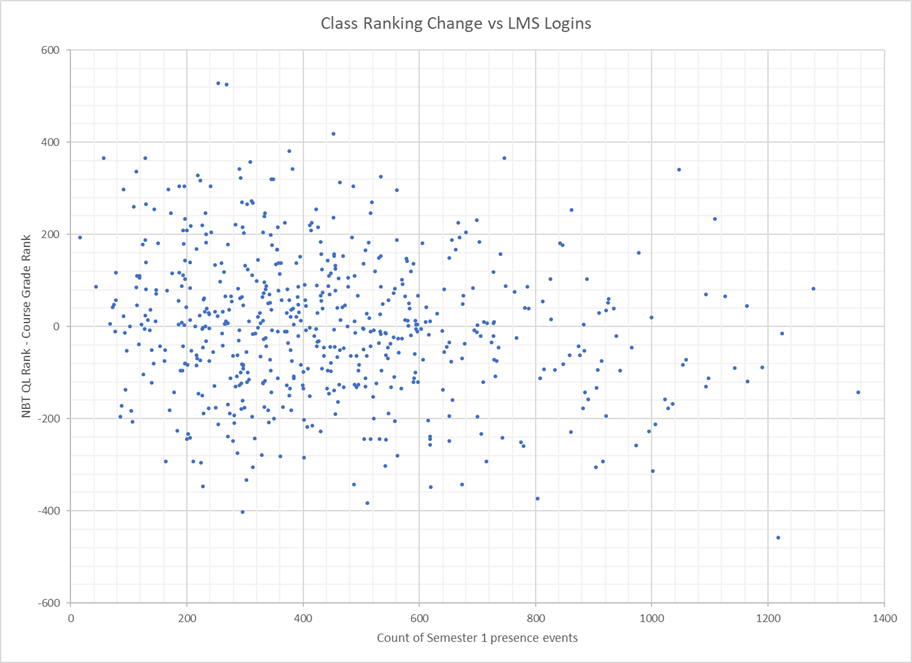
\includegraphics[scale=0.6]{./resources/figures/delta-class-rank.png}
    % \end{mdframed}
    \caption[\( \delta \) class rank vs LMS Logins]{\textbf{Figure \ref{fig-delta-rank}: \( \delta \) class rank vs LMS Logins.} An example of the correlation between \( \delta \) NBT QL ranking scores/course grades compared to LMS usage. As shown in Table \ref{tbl-correlation-variance}, the correlation coefficient between these two datasets is 0.17.}
    \label{fig-delta-rank}
\end{figure}

% Figures
\begin{figure}[H]
    \centering
    % \begin{mdframed}
    % \centering
    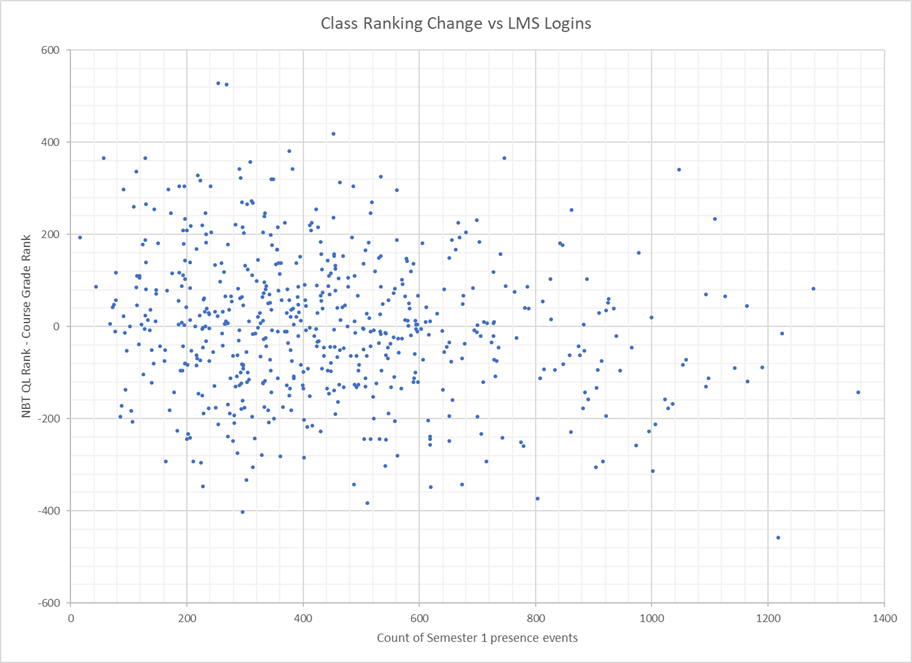
\includegraphics[scale=0.6]{./resources/figures/delta-class-rank.png}
    % \end{mdframed}
    \caption[\( \delta \) class rank vs LMS Logins]{\textbf{Figure \ref{fig-delta-rank}: \( \delta \) class rank vs LMS Logins.} An example of the correlation between \( \delta \) NBT QL ranking scores/course grades compared to LMS usage. As shown in Table \ref{tbl-correlation-variance}, the correlation coefficient between these two datasets is 0.17.}
    \label{fig-delta-rank}
\end{figure}
\begin{table}[H]
    \begin{threeparttable}
        \textbf{Table \ref{tbl-correlation-variance}}\par\medskip\par\medskip
        \caption[Correlation coefficients]{Assessment of correlation between the benchmark scores and course grades, and change in class ranking vs LMS usage per benchmark}
        \label{tbl-correlation-variance}
        \small
        \begin{tabularx}{\textwidth}{>{\hsize=1.4\hsize}X>{\hsize=0.8\hsize}Y>{\hsize=0.8\hsize}Y>{\hsize=0.8\hsize}Y}
            \toprule
            \mC{c}{Benchmark Used}                              & \mC{c}{Variance} & \mC{c}{2-Way Join} & \mC{c}{3-Way Join\tnote{\textsuperscript{4}}} \\
            \midrule
            Gr12 Eng                                            &                  & 0.15               & -0.02                                         \\
            Gr12 Sci                                            &                  & 0.08               & 0.06                                          \\
            Gr12 Mth                                            &                  & 0.25               & 0.02                                          \\
            NBT AL                                              &                  & 0.33               & -0.15                                         \\
            NBT QL                                              &                  & 0.48               & -0.17                                         \\
            NBT Mth                                             &                  & 0.45               & -0.02                                         \\
            \midrule
            Gr12 Results Avg\tnote{\textsuperscript{1}}         &                  & 0.17               &                                               \\
            Double Mth weight\tnote{\textsuperscript{2}}        &                  & 0.20               &                                               \\
            Double Mth \& Sci weight\tnote{\textsuperscript{3}} &                  & 0.16               &                                               \\
            \midrule
            NBT Results Avg                                     &                  & 0.49               &                                               \\
            Double NBT AL                                       &                  & 0.47               &                                               \\
            Double NBT QL                                       &                  & 0.50               &                                               \\
            Double NBT Mth                                      &                  & 0.50               &                                               \\
            Double NBT AL/QL                                    &                  & 0.48               &                                               \\
            Double NBT AL/Mth                                   &                  & 0.49               &                                               \\
            Double NBT QL/Mth                                   &                  & 0.50               &                                               \\
            \midrule
            Avg of NBT \& Gr12                                  &                  & 0.37               &                                               \\
            Double Gr 12 Mth weight                             &                  & 0.37               &                                               \\
            Double Gr12 Mth \& Sci weight                       &                  & 0.30               &                                               \\
            \bottomrule
        \end{tabularx}
        \scriptsize
        \begin{tablenotes}
            \item[\textsuperscript{1}]Original method used to benchmark incoming students
            \item[\textsuperscript{2}]Previously used method for benchmarking incoming students
            \item[\textsuperscript{3}]Currently used method of benchmarking incoming students
            \item[\textsuperscript{4}]\( \delta \)
        \end{tablenotes}
    \end{threeparttable}
\end{table}

\chapter{Conclusion}
\section{Summary}
1. However CouchDB itself has an opinionated implementation of MapReduce - which is used to build B+indexes instead of result sets as in hadoop. As such CouchDB's MapReduce is only useful when querying for analytics of a numerical nature.

2. CouchDB query times go down with more cluster nodes.

3. CouchDB is good for ... xxx


\section{Future work}
This project's scope is limited to a single approach to document joining, to working with a relatively small amount of data and and working in an environment that CouchDB is not necessarily targeted at. Aside from the fact that more case studies using CouchDB will greatly increase insight into how to use CouchDB more generally, there is scope for further development of the research presented here.

As mentioned previously, CouchDB views are optimized when using built-in reduce functions, with custom reduce functions performing most poorly on Windows machines. As this project was completed on the Windows OS, the analysis on how best to aggregate the different entities (grades, demographics and events) was confined to using just the \textit{\_stats} built in reduce function. The output of this function overlaps output of the other two built-in reduce functions (\textit{\_count}, \textit{\_sum} (and provides additional metrics). Using custom reduce functions would greatly increase the number of possible methods of joining entities since output of map functions would not be constrained to match the contracts of the built-in functions. Such an approach shouldn't be discounted considering that on platforms other than Windows, reduce function calculation (whether custom or built-in) represents a small percentage of computer resources used in view calculations overall (see appendix \ref{slack-1-nov}). And in any case, a system that utilizes CouchDB is likely to be based on a cluster of Linux machines rather than a single Windows machine.

Since, for this project, CouchDB was configured to run on a single Windows machine for this project, it would be worth investigating the benefit that clustering CoucDB across many separate nodes provides. Although the database was sharded (CouchDB is configured to use 8 shards by default) and so processed data in parallel, it is likely that deploying shards to separate servers would greatly increase performance and decrease indexing time. CouchDB disperses documents evenly across shards in a random fashion, suggesting that the workload of indexing the documents would be distributed evenly across all the shards of the database (see \ref{slack-7-nov}). It is likely that the larger benefits would be seen with increasing data sizes since there is first the cost of network interactions to overcome if shards were distributed across separate nodes.

There is also scope to develop a user interface for the \textit{nETL} application and launch a competitor to Microsoft's SSDT that is browser based and JSON-based.
\section*{Acknowledgments}
I would like to give special thanks to my project supervisor Associate Professor Sonia Berman - an extremely patient supervisor who had the foresight to push me (at great effort) in the direction that resulted in a completed MSc. I would also like to thank her for the effort she put in in terms of data acquisition and guiding me in designing the research topic. I would also like to thank Jane Hendry and Stephen Marquard for providing the data exports and scrubbing that such exports required. And lastly I would like to thank the many people who helped me with insights into the thesis topic and the technologies I used. Including: Stephanie Honchell, Patrick DeSomma, Guy Bedford, and many of the CouchDB community who took the time to reply to my messages over Slack.
\newpage

% Bibliogrpahy
\bibliographystyle{plain}
\bibliography{bibliography/msc_citations}

% Appendix
\begin{appendices}
    \chapter{nETL}
    \section{nETL Engine}
\subsection{Sequential Batch Iterator}
\label{netl-batch-generator}
\begin{minted}{javascript}
const extraction;
const batches = (function*() {
    var finished = false;
    while (!finished) {
        let data = [];
        for (let i = 0; i < batchSize; i++) {
            let datum = extraction.getNext();
            if (datum.done) {
                finished = true;
                break
            };
            data.push(datum.value);
        };
        log.info("Task : " + key + " : Batch extracted : Batch size : " + data.length);
        yield data;
    };
})();

// Iteratively generate next batch
batch = batches.next();
\end{minted}

\subsection{TaskManager Constructor}
\label{netl-taskmanager-constructor}
\begin{minted}{javascript}
function TaskManager(e, ts, l) {
    this.tasks = {};
    this.extractions = e;
    this.transformations = ts;
    this.loads = l;
};
TaskManager.prototype.newTask = function(task) { /* ... */ };
\end{minted}

\subsection{Main Application Module}
\label{netl-application-module}
\begin{minted}{javascript}
(function() {
    const _extractions = {};
    const _transformations = {};
    const _loads = {};        
    const _taskManager = new TaskManager(_extractions, _transformations, _loads);
    function _loadExtractionModule(eModule){/* ... */};
    function _loadTransformationModule(tModule){/* ... */};
    function _loadLoadModule(lModule){/* ... */};
    return {
        taskManager: _taskManager,
        loadExtractionModule: _loadExtractionModule,
        loadTransformationModule: _loadTransformationModule,
        loadLoadModule: _loadLoadModule
    };
})();
\end{minted}


\subsection{Recursive ETL Iteration}
\label{netl-recursive-iterator}
\begin{minted}{javascript}
const batches; // Assigned elsewhere
const transformations; // Assigned elsewhere
const load; // Assigned elsewhere
(function doEtlTask(self) {
    var payload = [];

    // Extract next batch
    batch = batches.next();
    if (!batch.done) {
        batch = batch.value;
        self.tasks[key]._itemsExtracted += batch.length;
        batch.forEach(function(item) {

            // Do transformations
            transformations.forEach(function(t) {
                item = t.transform(item);
            });
            if (item && item !== {}) payload.push(item);
        });

        // Load to destination
        load.batch(payload)
            .then(function(msg) {
                doEtlTask(self);
            });
    } else {
        // .. Handle end of task execution
    };
})(this); // Bound to TaskManager instance context
\end{minted}

\section{Extraction, Transformation, Load Modules}
\label{netl-modules}

\subsection{Loading a Module}
\label{netl-module-loading}
\begin{minted}{javascript}
// Load the module into memory
memoryObject[userModule.name] = userModule.exe;
// Invoke the module's closure
var loadedModule = memoryObject[userModule.Name].call(userModule);
// Genrate batch from extraction module
var batch = loadedModule.getNext()
// Do transformations on batch
batch = loadedModule.transform(batch);
// Load transformed batch
load.batch(batch).then(function(msg) {}).catch(function(msg) {});
// An example userModule (an extraction module)
userModule = (function() {
    function exe(configurationObj) {
        function getNext() { /* ... */};
        return {
            getNext: getNext
        };
    };
    return {
        name: "MODULE_NAME",
        exe: exe
    };
})();
\end{minted}


\subsection{FLATFILE}
\label{netl-extract-flatfile}
\begin{minted}{javascript}
'use strict';
const fs = require('fs');
const path = require('path');
/**
 * Configuration exampleL
 * "Extraction": {
 *     "Name": "FLATFILE",
 *     "path": "....csv",
 *     "skipHeaderRows": 1,
 *     "bufferSize": 65536,
 *     "batchSize": 10000,
 *     "startFrom": 0,
 *     "afterTaskRunCBs": []
 * }
 */
function FLATFILE() {
    const options = this;
    const skipItems = options.skipHeaderRows || 0;
    const LF = 10;
    const CR = 13;
    var bufferSize = options.bufferSize || 64 * 1024;
    var position = options.startFrom || 0;
    var lines = _readLines();
    var currentLine = -1;

    // Open the file to be extracted
    var fd;
    var fileStats;
    var filesize;
    var filepath;
    try {
        // Try absolute path
        try {
            filepath = path.normalize(options.path)
            fd = fs.openSync(filepath, 'r');
        } catch (error) {
            // Try relative path
            try {
                filepath = path.normalize(path.join(__dirname, options.path));
                fd = fs.openSync(filepath, 'r');
            } catch (error) {
                throw new Error("File at " + options.path + " cannot be found. Please check your configuration");
            };
        };
        fileStats = fs.fstatSync(fd);
        filesize = fileStats.size;
    } catch (error) {
        throw new Error(error.message);
    };

    /* PRIVATE method */
    function* _readLines() {
        var lineBuffer;
        while (position < filesize) {
            let remaining = filesize - position;
            if (remaining < bufferSize) bufferSize = remaining;
            let chunk = new Buffer(bufferSize);
            let bytesRead = fs.readSync(fd, chunk, 0, bufferSize, position);
            let curpos = 0;
            let startpos = 0;
            let lastbyte = null;
            let curbyte;
            while (curpos < bytesRead) {
                curbyte = chunk[curpos];
                if (curbyte === LF && lastbyte !== CR || curbyte === CR && curpos < bytesRead - 1) {
                    yield _concat(lineBuffer, chunk.slice(startpos, curpos));
                    lineBuffer = undefined;
                    startpos = curpos + 1;
                    if (curbyte === CR && chunk[curpos + 1] === LF) {
                        startpos++;
                        curpos++;
                    };
                } else if (curbyte === CR && curpos >= bytesRead - 1) {
                    lastbyte = curbyte;
                };
                curpos++;
            };
            position += bytesRead;
            if (startpos < bytesRead) {
                lineBuffer = _concat(lineBuffer, chunk.slice(startpos, bytesRead));
            };
        };
        // dump what ever is left in the buffer
        if (Buffer.isBuffer(lineBuffer)) yield lineBuffer;
    };

    /* PRIVATE method */
    function _concat(buffOne, buffTwo) {
        if (!buffOne) return buffTwo;
        if (!buffTwo) return buffOne;

        let newLength = buffOne.length + buffTwo.length;
        return Buffer.concat([buffOne, buffTwo], newLength);
    };

    /* PUBLIC method */
    function getNext() {
        var nextLine = lines.next();
        currentLine++;
        while (currentLine <= skipItems - 1) {
            nextLine = lines.next();
            currentLine++;
        };
        if (!nextLine.done) {
            nextLine.value = nextLine.value.toString();
        };
        return nextLine;
    };

    /* API */
    return {
        getNext: getNext
    };
};
module.exports = {
    name: "FLATFILE",
    exe: FLATFILE
};
\end{minted}

% Loads

\subsection{COUCHDB}
\label{netl-load-couchdb}
\begin{minted}{javascript}
'use strict';
const request = require('request');
/**
 * Configuration example:
 * "Load": {
 *     "Name": "COUCHDB",
 *     "username": "admin",
 *     "password": "password",
 *     "server": "localhost",
 *     "port": 5984,
 *     "ssl": false,
 *     "database": "msc",
 *     "afterTaskRunCBs": []
 * }
 */
function COUCHDB() {
    const options = this;
    const username = options.username || null;
    const password = options.password || null;
    const server = options.server || null;
    const protocol = (options.ssl) ? 'https' : 'http';
    const port = (options.port) ? (typeof options.port === 'number') ? options.port : 80 : 80;
    const db = options.database || null;
    const address = protocol + '://' + username + ':' + password + '@' + server + ':' + port + '/' + db;
    function batch(data) {
        var postData = { docs: data };
        var endpoint = '/_bulk_docs';
        var url = address + endpoint;
        return new Promise(function(fulfill, reject) {
            try {
                request({
                    uri: url,
                    method: 'POST',
                    headers: {
                        'Content-Type': 'application/json'
                    },
                    body: JSON.stringify(postData)
                }, function(err, res, body) {
                    var msg;
                    if (err) {
                        reject(err);
                    } else if (res.statusCode !== 201) {
                        reject(res.statusCode);
                    } else {
                        fulfill(res.statusCode);
                    };
                });
            } catch (e) {
                reject(e);
            };
        });
    };
    return {
        batch: batch
    };
};
module.exports = {
    name: 'COUCHDB',
    exe: COUCHDB
};
\end{minted}

% Transformations

\subsection{TEXT\_LINE\_TO\_OBJ}
\label{netl-trans-text-line-to-obj}
\begin{minted}{javascript}
'use strict';
const Readable = require('stream').Readable;
const csvParser = require('csv-parse/lib/sync');
/**
 * Using RFC 4180 CSV definition
 * Configuration example:
 * {
 *     "Name": "TEXT_LINE_TO_OBJ",
 *     "attributeNames": "<list of CSV headers>",
 *     "delimiter": ",",
 *     "textQualifier": "\"",
 *     "escapeChar": "\\",
 *     "afterTaskRunCBs": []
 * }
 */
function TEXT_LINE_TO_OBJ() {
    const t = this;
    const parseOptions = {
        auto_parse: true,
        auto_parse_date: true,
        columns: null,
        comment: '',
        delimiter: t.delimiter,
        escape: t.escapeChar,
        from: 0,
        to: 1,
        ltrim: true,
        rtrim: true,
        max_limit_on_data_read: 128000,
        quote: t.textQualifier,
        relax: true,
        relax_column_count: false,
        skip_empty_lines: true,
        skip_lines_with_empty_values: true
    };
    const keys = csvParser(t.attributeNames, parseOptions)[0];
    function transform(lines) {
        var retObjs = [];
        lines.forEach(function(line) {
            var values = csvParser(line, parseOptions)[0];
            var obj = Object.create(null);
            keys.forEach(function(el, i, arr) {
                obj[el] = values[i];
            });
            retObjs.push(obj);
        });
        return retObjs;
    };
    return {
        transform: transform
    };
};
module.exports = {
    name: 'TEXT_LINE_TO_OBJ',
    exe: TEXT_LINE_TO_OBJ
};
\end{minted}


\subsection{FILTER}
\label{netl-trans-filter}
\begin{minted}{javascript}
'use strict';
/**
 * Configuration looks like this:
 * filterOn: {"key1"; [<list of allowed values>], "key2": [...], ...}
 * filtering can either be done on objects or arrays since
 * arrays 'keys' are treated as indexes
 *
 * Configuration example:
 * {
 *     "Name": "FILTER",
 *     "filterOn": {
 *         "field1": [<list of allowed values>],
 *         "field2": [<list of allowed values>],
 *         etc...
 *     },
 *     "afterTaskRunCBs": []
 * }
 */
function FILTER() {
    const t = this;
    const filterOn = t.filterOn;
    function transform(batch) {
        const transformedBatch = [];
        batch.forEach(function(datum) {
            var includeThisObj = true;
            Object.keys(filterOn).forEach(function(key) {
                if (filterOn[key].indexOf(datum[key]) < 0) {
                    includeThisObj = false;
                }
            });
            if (includeThisObj) transformedBatch.push(datum);
        });
        return transformedBatch;
    };
    return {
        transform: transform
    };
};
module.exports = {
    name: 'FILTER',
    exe: FILTER
};
\end{minted}

\subsection{WHITELIST}
\label{netl-trans-whitelist}
\begin{minted}{javascript}
/**
 * Configuration example:
 * {
 *     "Name": "WHITELIST",
 *     "allowedAttributes": [
 *         "type_", "RegAcadYear", "anonIDnew", "Course", "Percent"
 *     ],
 *     "afterTaskRunCBs": []
 *     } 
 */
'use strict';
function WHITELIST() {
    const t = this;
    var allowedAttributes = t.allowedAttributes;
    function transform(docs) {
        var retDocs = [];
        docs.forEach(function(doc) {
            var newDoc = {};
            for (var attr in doc) {
                if (!doc.hasOwnProperty(attr)) continue;
                if (allowedAttributes.includes(attr)) newDoc[attr] = doc[attr];
            };
            if (Object.keys(newDoc).length !== 0) retDocs.push(newDoc);
        });
        return retDocs;
    };
    return {
        transform: transform
    };
};
module.exports = {
    name: 'WHITELIST',
    exe: WHITELIST
};
\end{minted}

\subsection{CREATE\_OBJ\_FIELD}
\label{netl-trans-create-obj-field}
\begin{minted}{javascript}
'use strict';
/**
 * Configuration example:
 * {
 *     "Name": "CREATE_OBJ_FIELD",
 *     "newAttributes": [
 *         ["type_", "courseGrade"]
 *     ],
 *     "afterTaskRunCBs": []
 * },
 */
function CREATE_OBJ_FIELD() {
    const t = this;
    function transform(batch) {
        const transformedBatch = JSON.parse(JSON.stringify(batch));
        transformedBatch.forEach(function(datum) {
            if (datum.length == 0) return;
            t.newAttributes.forEach(function(attr) {
                // Throw error if key already exists
                if (datum.hasOwnProperty(attr[0])) {
                    throw new Error("New property not allowed!");
                }
                datum[attr[0]] = attr[1]
            });
        });
        return transformedBatch;
    };
    return {
        transform: transform
    };
};
module.exports = {
    name: 'CREATE_OBJ_FIELD',
    exe: CREATE_OBJ_FIELD
};
\end{minted}
    \section{Configuration files}

\subsection{Result 1}
\label{netl-run1-config}
\begin{minted}{json}
[{
    "ID": "2014/15/16 FU: CSC1015F students",
    "Extraction": {
        "Name": "FLATFILE",
        "path": "C:/MSc/Data/Demographics/FU-CombinedGrades-2016Reg.csv",
        "skipHeaderRows": 1,
        "bufferSize": 65536,
        "batchSize": 10000,
        "startFrom": 0,
        "afterTaskRunCBs": []
    },
    "Transformations": [{
            "Name": "TEXT_LINE_TO_OBJ",
            "attributeNames": "anonIDnew,Career,Citizenship Residency,SA School,Eng Grd12 Fin Rslt,Math Grd12 Fin Rslt,Mth Lit Grd12 Fin Rslt,Adv Mth Grd12 Fin Rslt,Phy Sci Grd12 Fin Rslt,NBT AL Score,NBT QL Score,NBT Math Score,RegAcadYear",
            "delimiter": ",",
            "textQualifier": "\"",
            "escapeChar": "\\",
            "afterTaskRunCBs": []
        },
        {
            "Name": "FILTER",
            "filterOn": {
                "Career": ["UGRD", "First Year", "Second Year", "Third Year"],
                "Citizenship Residency": ["SA Citizen", "Permanent Resident", "C", "P"],
                "anonIDnew": ["list of student IDs for students that took CSC1015F in 2014/15/16"]
            },
            "afterTaskRunCBs": []
        },
        {
            "Name": "CREATE_OBJ_FIELD",
            "newAttributes": [
                ["type_", "demographic"]
            ],
            "afterTaskRunCBs": []
        },
        {
            "Name": "WHITELIST",
            "allowedAttributes": [
                "type_",
                "anonIDnew",
                "Eng Grd12 Fin Rslt",
                "Math Grd12 Fin Rslt",
                "Mth Lit Grd12 Fin Rslt",
                "Adv Mth Grd12 Fin Rslt",
                "Phy Sci Grd12 Fin Rslt",
                "NBT AL Score",
                "NBT QL Score",
                "NBT Math Score",
                "RegAcadYear"
            ],
            "afterTaskRunCBs": []
        }
    ],
    "Load": {
        "Name": "COUCHDB",
        "username": "admin",
        "password": "password",
        "server": "localhost",
        "port": 5984,
        "ssl": false,
        "database": "msc_run1",
        "afterTaskRunCBs": []
    }
}, {
    "ID": "2014/15/16 Grades: CSC1015F students",
    "Extraction": {
        "Name": "FLATFILE",
        "path": "C:/MSc/Data/Grades/CombinedGrades.csv",
        "skipHeaderRows": 1,
        "bufferSize": 65536,
        "batchSize": 10000,
        "startFrom": 0,
        "afterTaskRunCBs": []
    },
    "Transformations": [{
            "Name": "TEXT_LINE_TO_OBJ",
            "attributeNames": "DownloadedDate,RegAcadYear,RegTerm,anonIDnew,RegProgram,RegCareer,Degree,DegreeDescr,Subject,Catalog.,Course,CourseSuffix,Session,Percent,Symbol,UnitsTaken,CourseID,CourseDescr,CourseCareer,Faculty,Dept,MaximumCrseUnits,CourseCount,CourseLevel,CESM,Sub-CESM",
            "delimiter": ",",
            "textQualifier": "\"",
            "escapeChar": "\\",
            "afterTaskRunCBs": []
        },
        {
            "Name": "FILTER",
            "filterOn": {
                "RegCareer": ["UGRD"],
                "Course": ["CSC1015F"]
            },
            "afterTaskRunCBs": []
        },
        {
            "Name": "CREATE_OBJ_FIELD",
            "newAttributes": [
                ["type_", "courseGrade"]
            ],
            "afterTaskRunCBs": []
        },
        {
            "Name": "WHITELIST",
            "allowedAttributes": [
                "type_", "Course", "RegAcadYear", "anonIDnew", "Percent"
            ],
            "afterTaskRunCBs": []
        }
    ],
    "Load": {
        "Name": "COUCHDB",
        "username": "admin",
        "password": "password",
        "server": "localhost",
        "port": 5984,
        "ssl": false,
        "database": "msc_run1",
        "afterTaskRunCBs": []
    }
}]
\end{minted}

\subsection{Result 2}
\label{netl-run2-config}
\begin{minted}{json}
\end{minted}

\subsection{Result 3}
\label{netl-run3-config}
\begin{minted}{json}
\end{minted}

\subsection{Result 4}
\label{netl-run4-config}
\begin{minted}{json}
\end{minted}
    \chapter{CouchDB}
    \section{MapReduce Contract}
\label{couchdb-mapreduce-contracts}
\begin{minted}{text}
/**
 * Map function
 * @param  {Object} doc Each document in the database is passed in turn to the function
 * @return {null} Nothing is returned - key:value pairs are emitted (multiple pairs can be emitted per document)
 */
function(doc) {
    emit(someKey, someValue);
};

/**
 * Reduce function (javascript implementation of the _sum function shown)
 * @param  {Object[]} [keys] A list of [key, docId] pairs - key as from the map function, and key from the original doc
 * @param  {Object[]} values Output from the map function, or from the reduce function
 * @param  {Boolean} [rereduce] Indicates whether values are output from the map (rereduce = false) or reduce (rereduce = true) function
 * @return {[type]}
 */
function(keys, values, rereduce) {
    if (rereduce) {
        return values.reduce(function(a,b) {
            return a + b;
        }, 0);
    } else {
        return values.length;
    };
};
\end{minted}

\section{Sample Design Document}
\label{couchdb-design-doc-sample}
\begin{minted}{json}
{
    "_id": "_design/sample",
    "_rev": "xxxxx",
    "language": "javascript",
    "views": {
        "view1": {
            "map": "function(doc) { ... }",
            "reduce": "function(keys, values, rereduce) { ... }"
        },
        "view2": {
            "map": "function(doc) { ... }",
            "reduce": "_stats"            
        }
    },
    "shows": {
        "show1": "function(doc, req) { ... }",
        "show2": "function(doc, req) { ... }"
    },
    "lists": {
        "listFunc1": "function(head, req) { ... };",
        "listFunc2": "function(head, req) { ... };"
    },
    "updates": {
        "update1": "function(doc, req) { ... }",
        "update2": "function(doc, req) { ... }"
    },
    "filters": {
        "filter1": "function(doc, req) { ... }",
        "filter2": "function(doc, req) { ... }"
    },
    "validate_doc_update": "function(newDoc, oldDoc, userCtx, secObj) { ... }"
}
\end{minted}

\section{Design Document Functions}
\subsection{2-Way Join}
\subsubsection{Map Function}
\label{2-way-join-map-function}
\begin{minted}{text}
function(doc) {
    /* Compound key */
    var id;
    var course;
    var year;

    /* Decision tree */
    var type = doc.type_;
    switch (type) {
        case 'grade':

            /* Key */
            id = doc.anonIDnew;
            course = doc.Course;
            year = doc.RegAcadYear;

            /* Value */
            var percent = doc.Percent || '';

            /* Normalize the percent field to a number */
            if (typeof percent !== 'number') {
                if (typeof percent !== 'string') return;
                var percentCleaned = percent.toUpperCase().trim();

                /* Return if percent is a disallowed symbol */
                if ([
                        'ATT',
                        'DE',
                        'GIP',
                        'LOA',
                        'OS',
                        'OSS',
                        'PA',
                        'SAT',
                        'UNS',
                        'AB',
                        ''
                    ].indexOf(percentCleaned) >= 0) return;

                /* Get the percentage */
                switch (percentCleaned) {
                    case 'F':
                        percent = 40;
                        break;
                    case 'DPR':
                        percent = 30;
                        break;
                    case 'INC':
                        percent = 30;
                        break;
                    case 'UF':
                        percent = 49;
                        break;
                    case 'UP':
                        percent = 45;
                        break;
                    default:
                        /* Convert percent to number */
                        percent = parseFloat(percent.substring(0, percent.length - 1));
                        if (isNaN(percent)) return;
                        break;
                };
            };

            /* Output */
            emit([id, course, year], percent);
            break;

        case 'benchmark':

            /* Key */
            id = doc.anonIDnew;
            course = 0;
            year = 0;

            /* Value (each index corresponds to a benchmark) */
            var benchmarks = [0, 0, 0, 0, 0, 0, 0, 0];

            /* Normalize symbols to numbers */
            var fuDictionary = {
                "A*": 90,
                "A": 80,
                "B": 70,
                "C": 60,
                "D": 55,
                "E": 50
            };

            function getDemographicGrade(gr) {
                var g = parseInt(gr);
                var retG;
                if (isNaN(g)) { // True for sumbols
                    if (typeof gr !== 'string') return 0;
                    retG = fuDictionary[gr.toUpperCase().trim()] || 0;
                } else {
                    retG = g;
                };
                return retG;
            };

            // Gr12 Eng
            var gEng12 = getDemographicGrade(doc["Eng Grd12 Fin Rslt"] || "");
            benchmarks[0] = gEng12;

            // Gr12 Sci
            var gSci12 = getDemographicGrade(doc["Phy Sci Grd12 Fin Rslt"] || "");
            benchmarks[1] = gSci12;

            // Gr12 Mth
            var gMth12 = getDemographicGrade(doc["Math Grd12 Fin Rslt"] || "");
            benchmarks[2] = gMth12;

            // Gr12 Mth Lit
            var gMthLit12 = getDemographicGrade(doc["Mth Lit Grd12 Fin Rslt"] || "");
            benchmarks[3] = gMthLit12;

            // Gr12 Mth Adv
            var gMthAdv12 = getDemographicGrade(doc["Adv Mth Grd12 Fin Rslt"] || "");
            benchmarks[4] = gMthAdv12;

            // NBT AL
            var gNbtAl = getDemographicGrade(doc["NBT AL Score"] || "");
            benchmarks[5] = gNbtAl;

            // NBT QL
            var gNbtQl = getDemographicGrade(doc["NBT QL Score"] || "");
            benchmarks[6] = gNbtQl;

            // NBT Mth
            var gNbtMth = getDemographicGrade(doc["NBT Math Score"] || "");
            benchmarks[7] = gNbtMth;

            /* Output */
            emit([id, course, year], benchmarks);
            break;

        default:
            break;
    };
};
\end{minted}

\subsubsection{List Function}
\label{2-way-join-list-function}
\begin{minted}{text}
function(head, req) {
    provides('csv', function() {
        /* Send the headers */
        var headers = "Year,StudentAnonID,Course,Course %,Gr12 Eng %,Gr12 Sci %,Gr12 Mth %,Gr12 Mth Lit %,Gr12 Mth Adv %,NBT AL %,NBT QL %,NBT Mth %";
        send(headers);

        /* Helper function; send current year */
        function sendLine(obj) {
            if (obj.benchmark && obj.grade) {
                var line =
                    "\n" + obj.year +
                    "," + obj.id +
                    "," + obj.course +
                    "," + obj["Course %"] +
                    "," + obj["Gr12 Eng %"] +
                    "," + obj["Gr12 Sci %"] +
                    "," + obj["Gr12 Mth %"] +
                    "," + obj["Gr12 Mth Lit %"] +
                    "," + obj["Gr12 Mth Lit %"] +
                    "," + obj["NBT AL %"] +
                    "," + obj["NBT QL %"] +
                    "," + obj["NBT Mth %"];
                send(line);
            };
        };

        /* Current function scope variables */
        var currentStudent = null;
        var currentYear = null;
        var currentLine = {};
        var key;
        var id;
        var course;
        var year;
        var value;

        /* Iterate through view results */
        while (row = getRow()) {

            /* Key */
            key = row.key;
            id = key[0];
            course = key[1];
            year = key[2];

            /* Value */
            value = row.value;

            /* Send previous line if it's a new student and then reset id */
            if (currentStudent !== id) {
                sendLine(currentLine);
                currentLine = {};
                currentStudent = id;
            };

            /* Append to/adjust current line */
            var type = (course === 0 && year === 0) ? 'benchmark' : 'grade';
            switch (type) {
                case 'benchmark':
                    currentLine.benchmark = true;
                    currentLine.id = id;
                    currentLine["Gr12 Eng %"] = value[0];
                    currentLine["Gr12 Sci %"] = value[1];
                    currentLine["Gr12 Mth %"] = value[2];
                    currentLine["Gr12 Mth Lit %"] = value[3];
                    currentLine["Gr12 Mth Adv %"] = value[4];
                    currentLine["NBT AL %"] = value[5];
                    currentLine["NBT QL %"] = value[6];
                    currentLine["NBT Mth %"] = value[7];
                    break;

                case 'grade':

                    /* Send previous line if it's a new year */
                    if (currentYear !== year) {
                        sendLine(currentLine);
                        currentYear = year;
                    };

                    currentLine.grade = true;
                    currentLine.id = id; // In case no demographic doc exists
                    currentLine.year = year;
                    currentLine.course = course;
                    currentLine["Course %"] = value[0];
                    break;

                default:
                    send({ error: "Document type unexpected" });
                    break;
            };
        };
    });
};
\end{minted}

\subsection{3-Way Join}
\subsubsection{Map Function}
\label{3-way-join-map-function}
\begin{minted}{text}
function(doc) {
    /* Compound key */
    var id;
    var course;
    var year;

    /* Decision tree */
    var type = doc.type_;
    switch (type) {
        case 'grade':
            /* Key */
            id = doc.anonIDnew;
            course = doc.Course;
            year = doc.RegAcadYear;

            /* Value */
            var percent = doc.Percent || '';

            /* Normalize the percent field to a number */
            if (typeof percent !== 'number') {
                if (typeof percent !== 'string') return;
                var percentCleaned = percent.toUpperCase().trim();

                /* Return if percent is a disallowed symbol */
                if ([
                        'ATT',
                        'DE',
                        'GIP',
                        'LOA',
                        'OS',
                        'OSS',
                        'PA',
                        'SAT',
                        'UNS',
                        'AB',
                        ''
                    ].indexOf(percentCleaned) >= 0) return;

                /* Get the percentage */
                switch (percentCleaned) {
                    case 'F':
                        percent = 40;
                        break;
                    case 'DPR':
                        percent = 30;
                        break;
                    case 'INC':
                        percent = 30;
                        break;
                    case 'UF':
                        percent = 49;
                        break;
                    case 'UP':
                        percent = 45;
                        break;
                    default:
                        /* Convert percent to number */
                        percent = parseFloat(percent.substring(0, percent.length - 1));
                        if (isNaN(percent)) return;
                        break;
                };
            };

            /* Output */
            emit([id, course, year], percent);
            break;

        case 'benchmark':
            /* Key */
            id = doc.anonIDnew;
            course = 0;
            year = 0;

            /* Value (each index corresponds to a benchmark) */
            var benchmarks = [0, 0, 0, 0, 0, 0, 0, 0];

            /* Normalize symbols to numbers */
            var fuDictionary = {
                "A*": 90,
                "A": 80,
                "B": 70,
                "C": 60,
                "D": 55,
                "E": 50
            };

            function getDemographicGrade(gr) {
                var g = parseInt(gr);
                var retG;
                if (isNaN(g)) { // True for sumbols
                    if (typeof gr !== 'string') return 0;
                    retG = fuDictionary[gr.toUpperCase().trim()] || 0;
                } else {
                    retG = g;
                };
                return retG;
            };

            // Gr12 Eng
            var gEng12 = getDemographicGrade(doc["Eng Grd12 Fin Rslt"] || "");
            benchmarks[0] = gEng12;

            // Gr12 Sci
            var gSci12 = getDemographicGrade(doc["Phy Sci Grd12 Fin Rslt"] || "");
            benchmarks[1] = gSci12;

            // Gr12 Mth
            var gMth12 = getDemographicGrade(doc["Math Grd12 Fin Rslt"] || "");
            benchmarks[2] = gMth12;

            // Gr12 Mth Lit
            var gMthLit12 = getDemographicGrade(doc["Mth Lit Grd12 Fin Rslt"] || "");
            benchmarks[3] = gMthLit12;

            // Gr12 Mth Adv
            var gMthAdv12 = getDemographicGrade(doc["Adv Mth Grd12 Fin Rslt"] || "");
            benchmarks[4] = gMthAdv12;

            // NBT AL
            var gNbtAl = getDemographicGrade(doc["NBT AL Score"] || "");
            benchmarks[5] = gNbtAl;

            // NBT QL
            var gNbtQl = getDemographicGrade(doc["NBT QL Score"] || "");
            benchmarks[6] = gNbtQl;

            // NBT Mth
            var gNbtMth = getDemographicGrade(doc["NBT Math Score"] || "");
            benchmarks[7] = gNbtMth;

            /* Output */
            emit([id, course, year], benchmarks);
            break;

        case 'event':
            var date = new Date(doc.event_date);
            var epoch = date.getTime();

            /* Key */
            id = doc.uct_id;
            course = 0;
            year = date.getFullYear();

            /* Value */
            var event = [0, 0];

            /* Midpoint =  Sunday, July 17, 2016 10:00:00 PM */
            var midDate = 1468792800000
            var semester = (epoch - midDate >= 0) ? 2 : 1;
            if (semester === 1) {
                event[0] = 1;
            } else {
                event[1] = 1;
            };

            /* Output */
            emit([id, course, year], event);
            break;

        default:
            break;
    };
};
\end{minted}

\subsubsection{List Function}
\label{3-way-join-list-function}
\begin{minted}{text}
function(head, req) {
    provides('csv', function() {
        /* Send the headers */
        var headers = "Year,StudentAnonID,Course,Course %,Gr12 Eng %,Gr12 Sci %,Gr12 Mth %,Gr12 Mth Lit %,Gr12 Mth Adv %,NBT AL %,NBT QL %,NBT Mth %,S1 Events, S2 Events";
        send(headers);

        /* Helper function; send current year */
        function sendLine(obj) {
            if (obj.benchmark && obj.grade) {
                var line =
                    "\n" + obj.year +
                    "," + obj.id +
                    "," + obj.course +
                    "," + obj["Course %"] +
                    "," + obj["Gr12 Eng %"] +
                    "," + obj["Gr12 Sci %"] +
                    "," + obj["Gr12 Mth %"] +
                    "," + obj["Gr12 Mth Lit %"] +
                    "," + obj["Gr12 Mth Lit %"] +
                    "," + obj["NBT AL %"] +
                    "," + obj["NBT QL %"] +
                    "," + obj["NBT Mth %"] +
                    "," + obj.S1 +
                    "," + obj.S2;
                send(line);
            };
        };

        /* Current function scope variables */
        var currentStudent = null;
        var currentYear = null;
        var currentLine = {};
        var key;
        var id;
        var course;
        var year;
        var value;

        /* Iterate through view results */
        while (row = getRow()) {

            /* Key */
            key = row.key;
            id = key[0];
            course = key[1];
            year = key[2];

            /* Value */
            value = row.value;

            /* Send previous line if it's a new student and then reset id */
            if (currentStudent !== id) {
                sendLine(currentLine);
                currentLine = {};
                currentStudent = id;
            };

            /* Append to/adjust current line */
            var type = (course === 0 && year === 0) ?
                'benchmark' : ((course === 0) ?
                    'event' : 'grade');

            switch (type) {
                case 'benchmark':
                    currentLine.benchmark = true;
                    currentLine.id = id;
                    currentLine["Gr12 Eng %"] = value[0];
                    currentLine["Gr12 Sci %"] = value[1];
                    currentLine["Gr12 Mth %"] = value[2];
                    currentLine["Gr12 Mth Lit %"] = value[3];
                    currentLine["Gr12 Mth Adv %"] = value[4];
                    currentLine["NBT AL %"] = value[5];
                    currentLine["NBT QL %"] = value[6];
                    currentLine["NBT Mth %"] = value[7];
                    break;

                case 'event':
                    currentLine.event = true;
                    currentLine.id = id;
                    currentLine.year = year // In case no benchmark or grade exists
                    currentLine.S1 = value[0];
                    currentLine.S2 = value[1];
                    break;

                case 'grade':

                    /* Send previous line if it's a new year */
                    if (currentYear !== year) {
                        sendLine(currentLine);
                        currentYear = year;
                    };

                    currentLine.grade = true;
                    currentLine.id = id; // In case no benchmark or event exists
                    currentLine.year = year;
                    currentLine.course = course;
                    currentLine["Course %"] = value;
                    break;

                default:
                    send({ error: "Document type unexpected" });
                    break;
            };
        };
    });
};
\end{minted}
    \chapter{Unit Tests}
    \label{unit-tests}
    \subsection{FLATFILE Extraction}
\label{FLATFILE-tests}
\begin{minted}{text}
'use strict';
const assert = require('assert');
const path = require('path');

const e = {
    "Name": "FLATFILE",
    "path": path.join(__dirname, '/test.csv'),
    "skipHeaderRows": 1,
    "bufferSize": 65536,
    "batchSize": 1,
    "startFrom": 0,
    "afterTaskRunCBs": []
};

describe('CSV Parsing', function() {
    it("Returns all the lines in a CSV", function() {
        const m = require('../index.js').exe.call(e);
        var row = m.getNext();
        var c = 1;
        while (!row.done) {
            c++;
            row = m.getNext();
        };
        assert.equal(c, 16);
    });
    it("Returns single rows at a time", function() {
        const m = require('../index.js').exe.call(e);
        var row = m.getNext();
        for (let i = 0; i < 5; i++) {
            row = m.getNext();
        };
        const vals = row.value;
        assert.equal('Row 7 Column 1,Row 7 Column 2,Row 7 Column 3,Row 7 Column 4,Row 7 Column 5', vals);
    });
});
\end{minted}
\section{nETL COUCHDB Load}
\label{COUCHDB-tests}
\begin{minted}{text}
'use strict';
const assert = require('assert');

const data = [
    { a: "a", b: "b", c: "c" },
    { a: "a2", b: "b2", c: "c2" },
    { a: "a3", b: "b3", c: "c3" }
];

describe('CouchDB loading:', function() {
    it("Batch load recieves 201 response", function() {
        const l = {
            "Name": "COUCHDB",
            "username": "admin",
            "password": "password",
            "server": "localhost",
            "port": 5984,
            "ssl": false,
            "database": "test"
        };
        const m = require('../index.js').exe.call(l);
        m.batch(data)
            .then(function(res) {
                assert.equal(res, 201);
            })
            .catch(function(msg) {
                assert.fail("Loading data into CouchDB did not succeed: " + msg);
            })
    });
});
\end{minted}
\section{nETL TEXT\_LINE\_TO\_OBJ Transformation}
\label{TEXT_LINE_TO_OBJ-tests}
\begin{minted}{javascript}
'use strict';
const assert = require('assert');

describe('CSV values:', function() {
    describe('Are correctly split:', function() {
        const t = {
            "Name": "TEXT_LINE_TO_OBJ",
            "attributeNames": "h1,h2,h3",
            "delimiter": ",",
            "textQualifier": "\"",
            "escapeChar": "\\",
            "afterTaskRunCBs": []
        };
        it(`"a,1,true" is split into 3 ordered columns via a standard delimiter (,)`, function() {
            const m = require('../index.js').exe.call(t);
            const result = m.transform("a,1,true");
            const vals = Object.values(result);
            const valCount = vals.length;
            assert.equal(3, valCount);
            assert.equal(vals[0], 'a');
            assert.equal(vals[1], '1');
            assert.equal(vals[2], 'true');
        });
        it(`"a;1;true" is split into 3 ordered columns via alternative delimiter (;)`, function() {
            const t = {
                "Name": "TEXT_LINE_TO_OBJ",
                "delimiter": ";",
                "attributeNames": "h1;h2;h3",
                "textQualifier": "\"",
                "escapeChar": "\\",
                "afterTaskRunCBs": []
            };
            var m = require('../index.js').exe.call(t);
            var result = m.transform("a;1;true");
            const vals = Object.values(result);
            const valCount = vals.length;
            assert.equal(3, valCount);
            assert.equal(vals[0], 'a');
            assert.equal(vals[1], '1');
            assert.equal(vals[2], 'true');
        });
        it(`"a;1;true" is split into 3 ordered columns via a complex delimiter (|~|)`, function() {
            var t = {
                "Name": "TEXT_LINE_TO_OBJ",
                "delimiter": "|~|",
                "attributeNames": "h1|~|h2|~|h3",
                "textQualifier": "\"",
                "escapeChar": "\\",
                "afterTaskRunCBs": []
            };
            var m = require('../index.js').exe.call(t);
            var result = m.transform("a|~|1|~|true");
            const vals = Object.values(result);
            const valCount = vals.length;
            assert.equal(3, valCount);
            assert.equal(vals[0], 'a');
            assert.equal(vals[1], '1');
            assert.equal(vals[2], 'true');
        });
        it(`Headers are matched to the correct columns`, function() {
            const m = require('../index.js').exe.call(t);
            const result = m.transform("a,1,true");
            assert.equal(result['h1'], 'a');
            assert.equal(result['h2'], '1');
            assert.equal(result['h3'], 'true');
        });
        it(`JavaScript objects are created`, function() {
            const m = require('../index.js').exe.call(t);
            const result = m.transform("a,1,true");
            assert.equal('object', typeof result);
        });
    });

    describe('Are parsed corectly:', function() {
        it('Values can be wrapped by a qualifier (")', function() {
            var t = {
                "Name": "TEXT_LINE_TO_OBJ",
                "delimiter": ",",
                "attributeNames": "\"h1\",\"h2\",\"h3\"",
                "textQualifier": "\"",
                "escapeChar": "\\",
                "afterTaskRunCBs": []
            };
            var m = require('../index.js').exe.call(t);
            var result = m.transform("v1,\"2\",true");
            assert.equal(result.h1, 'v1');
            assert.equal(result.h2, 2);
            assert.equal(result.h3, 'true');
        });
        it("Date conversion is implicit", function() {
            var t = {
                "Name": "TEXT_LINE_TO_OBJ",
                "delimiter": ",",
                "attributeNames": "\"h1\",\"h2\",\"h3\"",
                "textQualifier": "\"",
                "escapeChar": "\\",
                "afterTaskRunCBs": []
            };
            var m = require('../index.js').exe.call(t);
            var result = m.transform("v1,\"2016-02-08 12:47:45\",true");
            assert.equal(result.h1, 'v1');
            assert.equal(Object.prototype.toString.call(result['h2']), '[object Date]');
            assert.equal(result.h3, 'true');
        });
    });
});
\end{minted}
\section{nETL FILTER Transformation}
\label{FILTER-tests}
\begin{minted}{javascript}
'use strict';
const assert = require('assert');

const objs = [
    { a: "a", b: "b", c: "c" },
    { a: "a2", b: "b2", c: "c2" },
    { a: "a3", b: "b3", c: "c3" }
];

describe('Objects can be filtered by:', function() {
    it("A single value for a single attribute:", function() {
        const t = {
            "Name": "FILTER",
            "filterOn": {
                "a": ["a"]
            }
        };
        const m = require('../index.js').exe.call(t);
        const result = objs.map(function(obj) {
            return m.transform(obj)
        });
        assert.equal(objs[0], result[0]);
        assert.equal(null, result[1]);
        assert.equal(null, result[2]);
    });
    it("Multiple values for a single attribute:", function() {
        const t = {
            "Name": "FILTER",
            "filterOn": {
                "a": ["a", "a2"]
            }
        };
        const m = require('../index.js').exe.call(t);
        const result = objs.map(function(obj) {
            return m.transform(obj)
        });
        assert.equal(objs[0], result[0]);
        assert.equal(objs[1], result[1]);
        assert.equal(null, result[2]);
    });
    it("A single values for a multiple attribute:", function() {
        const t = {
            "Name": "FILTER",
            "filterOn": {
                "a": ["a"],
                "b": ["b"],
            }
        };
        const m = require('../index.js').exe.call(t);
        const result = objs.map(function(obj) {
            return m.transform(obj)
        });
        assert.equal(objs[0], result[0]);
        assert.equal(null, result[1]);
        assert.equal(null, result[2]);
    });
    it("Multiple values for a multiple attribute:", function() {
        const t = {
            "Name": "FILTER",
            "filterOn": {
                "a": ["a", "a2"],
                "b": ["b", "b2"],
            }
        };
        const m = require('../index.js').exe.call(t);
        const result = objs.map(function(obj) {
            return m.transform(obj)
        });
        assert.equal(objs[0], result[0]);
        assert.equal(objs[1], result[1]);
        assert.equal(null, result[2]);
    });
    it("Filtered objects meet all filter conditions:", function() {
        const t = {
            "Name": "FILTER",
            "filterOn": {
                "a": ["a", "a2"],
                "b": ["b"],
            }
        };
        const m = require('../index.js').exe.call(t);
        const result = objs.map(function(obj) {
            return m.transform(obj)
        });
        assert.equal(objs[0], result[0]);
        assert.equal(null, result[1]);
        assert.equal(null, result[2]);
    });
});
\end{minted}
\section{nETL CREATE\_OBJECT\_FIELD Transformation}
\label{CREATE_OBJECT_FIELD-tests}
\begin{minted}{text}
'use strict';
const assert = require('assert');

const objs = [
    { a: "a", b: "b", c: "c" },
    { a: "a2", b: "b2", c: "c2" },
    { a: "a3", b: "b3", c: "c3" }
];

describe('Attributes can be appended to objects:', function() {
    it("A single attribute can be added to objects:", function() {
        const t = {
            "Name": "CREATE_OBJ_FIELD",
            "newAttributes": [
                ["type_", "test"]
            ]
        };
        const m = require('../index.js').exe.call(t);
        const result = objs.map(function(obj) {
            return m.transform(obj)
        });
        result.forEach(function(item) {
            assert.strictEqual(item.type_, "test");
        });
    });
    it("Multiple attribute can be added to objects:", function() {
        const t = {
            "Name": "CREATE_OBJ_FIELD",
            "newAttributes": [
                ["type_", "test"],
                ["otherAttribute", "test2"],
            ]
        };
        const m = require('../index.js').exe.call(t);
        const result = objs.map(function(obj) {
            return m.transform(obj)
        });
        result.forEach(function(item) {
            assert.strictEqual(item.type_, "test");
            assert.strictEqual(item.otherAttribute, "test2");
        });
    });
    it("New key:value pairs added to objects are type sensitive:", function() {
        const t = {
            "Name": "CREATE_OBJ_FIELD",
            "newAttributes": [
                ["bool", false],
                ["bool2", true],
                ["int", 10]
            ]
        };
        const m = require('../index.js').exe.call(t);
        const result = objs.map(function(obj) {
            return m.transform(obj)
        });
        result.forEach(function(item) {
            assert.strictEqual(item.bool, false);
            assert.strictEqual(item.bool2, true);
            assert.strictEqual(item.int, 10);
        });
    });
});
\end{minted}
\section{nETL WHITELIST Transformation}
\label{WHITELIST-tests}
\begin{minted}{javascript}
'use strict';
const assert = require('assert');

const objs = [
    { a: "a", b: "b", c: "c" },
    { a: "a2", b: "b2", c: "c2" },
    { a: "a3", b: "b3", c: "c3" }
];

describe('Attributes can be appended to objects:', function() {
    it("A single attribute can be added to objects:", function() {
        const t = {
            "Name": "CREATE_OBJ_FIELD",
            "newAttributes": [
                ["type_", "test"]
            ]
        };
        const m = require('../index.js').exe.call(t);
        const result = objs.map(function(obj) {
            return m.transform(obj)
        });
        result.forEach(function(item) {
            assert.strictEqual(item.type_, "test");
        });
    });
    it("Multiple attribute can be added to objects:", function() {
        const t = {
            "Name": "CREATE_OBJ_FIELD",
            "newAttributes": [
                ["type_", "test"],
                ["otherAttribute", "test2"],
            ]
        };
        const m = require('../index.js').exe.call(t);
        const result = objs.map(function(obj) {
            return m.transform(obj)
        });
        result.forEach(function(item) {
            assert.strictEqual(item.type_, "test");
            assert.strictEqual(item.otherAttribute, "test2");
        });
    });
    it("New key:value pairs added to objects are type sensitive:", function() {
        const t = {
            "Name": "CREATE_OBJ_FIELD",
            "newAttributes": [
                ["bool", false],
                ["bool2", true],
                ["int", 10]
            ]
        };
        const m = require('../index.js').exe.call(t);
        const result = objs.map(function(obj) {
            return m.transform(obj)
        });
        result.forEach(function(item) {
            assert.strictEqual(item.bool, false);
            assert.strictEqual(item.bool2, true);
            assert.strictEqual(item.int, 10);
        });
    });
});
\end{minted}
\section{CouchDB Map and List Function}
\label{Map-List-tests}
\begin{minted}{text}
'use strict';
const path = require('path');
const fs = require('fs');
const assert = require('assert');

// Docs
const docs = [
    // benchmarks
    { "anonIDnew": 2448646, "Eng Grd12 Fin Rslt": 82, "Math Grd12 Fin Rslt": 94, "Mth Lit Grd12 Fin Rslt": "", "Adv Mth Grd12 Fin Rslt": "", "Phy Sci Grd12 Fin Rslt": 96, "NBT AL Score": 64, "NBT QL Score": 72, "NBT Math Score": 86, "RegAcadYear": 2016, "type_": "benchmark" },

    // events
    // { "event_date": "2016-04-15T07:53:19.000Z", "event_id": 281, "uct_id": 2448649, "site_key": 20627, "type_": "event" },

    // grades
    { "RegAcadYear": 2016, "anonIDnew": 2448646, "Course": "CSC1015F", "Percent": "F", "type_": "grade" },
    { "RegAcadYear": 2014, "anonIDnew": 2448647, "Course": "CSC1015F", "Percent": "DPR", "type_": "grade" },
    { "RegAcadYear": 2014, "anonIDnew": 2448648, "Course": "CSC1015F", "Percent": "INC", "type_": "grade" },
    { "RegAcadYear": 2014, "anonIDnew": 2448649, "Course": "CSC1015F", "Percent": "UF", "type_": "grade" },
    { "RegAcadYear": 2014, "anonIDnew": 2448650, "Course": "CSC1015F", "Percent": "UP", "type_": "grade" },
    { "RegAcadYear": 2014, "anonIDnew": 2448651, "Course": "CSC1015F", "Percent": 99, "type_": "grade" },
    { "RegAcadYear": 2014, "anonIDnew": 2448652, "Course": "CSC1015F", "Percent": "OS", "type_": "grade" }
];

// Load CouchDB functions into environment
const maps = {};
const lists = {};
eval(`maps["2-way"] = ${fs.readFileSync(__dirname + '/../two-way-join/views/2-way-join.csv/map.js')}`);
eval(`maps["3-way"] = ${fs.readFileSync(__dirname + '/../three-way-join/views/3-way-join.csv/map.js')}`);
eval(`lists["2-way"] = ${fs.readFileSync(__dirname + '/../two-way-join/lists/2-way-join.js')}`);
eval(`lists["3-way"] = ${fs.readFileSync(__dirname + '/../three-way-join/lists/3-way-join.js')}`);

/* Hold results emitted by Map function (reset by each test) */
var mappedDocs;

/* Emulate the 'emit' function provided by CouchDB */
function emit(v1, v2) {
    mappedDocs.push([v1, v2]);
};

/* Emulate CouchDB provides function */
function provides(str, cb) { cb(); }

/* Hold results emitted by List function (reset by each test) */
var listResuts;

/* Emulate the 'send' function provided by CouchDB */
function send(str) {
    listResuts.push(str);
};

/* Emulate the 'getRow' function provided by CouchDB */
const iterator = (function*() {
    var i = 0;
    while (docs[i]) {
        yield docs[i];
        i++;
    };
})();

function getRow() {
    var currentRow = iterator.next();
    if (currentRow.done) {
        return false;
    } else {
        mappedDocs = [];
        maps["2-way"](currentRow.value);
        if (mappedDocs[0]) return { key: mappedDocs[0][0], value: mappedDocs[0][1] }
    };
};

/* Do tests */
describe('2-Way Join:', function() {
    describe('Map Function', function() {
        mappedDocs = [];
        docs.forEach(function(doc, i) {
            maps["2-way"](doc);
        });
        it("Emits the correct keys for grade and benchmark docs", function() {
            assert.deepEqual(mappedDocs[0][0], [2448646, 0, 0]);
            assert.deepEqual(mappedDocs[1][0], [2448646, 'CSC1015F', 2016]);
            assert.deepEqual(mappedDocs[2][0], [2448647, 'CSC1015F', 2014]);
        });
        it("Translates grades to numbers correctly", function() {
            assert.deepEqual(mappedDocs[0][1], [82, 96, 94, 0, 0, 64, 72, 86]);
            assert.equal(mappedDocs[2][1], 30);
            assert.equal(mappedDocs[3][1], 30);
            assert.equal(mappedDocs[4][1], 49);
            assert.equal(mappedDocs[5][1], 45);
            assert.equal(mappedDocs[6][1], 99);
        });
        it("Doesn't emit docs for ignored symbols", function() {
            assert.equal(mappedDocs[7], undefined);
        });
    });
    describe('List Function', function() {
        listResuts = [];
        it('Run generator..', function() {
            lists["2-way"](null, null);
        });
        it('Headers should be emitted', function() {
            assert.deepEqual(listResuts[1], '\n2016,2448646,CSC1015F,40,82,96,94,0,0,64,72,86');
        });
        it('Join of student grade and benchmark should be correct', function() {
            assert.deepEqual(listResuts[1], '\n2016,2448646,CSC1015F,40,82,96,94,0,0,64,72,86');
        });
    });
});

describe('3-Way Join:', function() {
    describe('Map Function', function() {
        it("...", function() {
            mappedDocs = [];
        });
    });
    describe('List Function', function() {
        it('...', function() {

        });
    });
});
\end{minted}
    \chapter{Logs}
    On Windows OS, CouchDB logs are located at 'C:\\CouchDB\\var\\log\\couchdb.log'. To look for logs related to indexing times, the following code was used (note that this is run on a Linux termninal that has access to underlying Windows file system).

\textit{\textbf{Retreiving CouchDB logs}}
\begin{minted}{sh}
grep -E '2017-12-13.*Starting\s.*_design/msc|2017-12-13.*Index\supdate\sfinished.*_design/msc' couchdb.log;
tail -f couchdb.log | grep -E '2017-12-15.*Starting\s.*_design/msc|2017-12-15.*Index\supdate\sfinished.*_design/msc';
tail -f couchdb.log --lines 100 | grep -E 'Starting\sindex\supdate.*_design/msc|.*Index\supdate\sfinished.*_design/msc'
\end{minted}

\textit{\textbf{Retreiving nETL logs}}
\begin{minted}{sh}
grep "completed" netl.log;
\end{minted}


\section{Result 1}
\textit{\textbf{nETL logs}}
\begin{verbatim}
1513328289697 : INFO : "Task : Student Demographics for CSC1015F (2014/15/66) : Task completed in 2.488 seconds : 12219 Items extracted : 1381 Items processed"
1513328325367 : INFO : "Task : Student Grades for CSC1015F  (2016, 2015, 2014) : Task completed in 37.684 seconds : 513872 Items extracted : 1891 Items processed"
\end{verbatim}

\textit{\textbf{CouchDB logs}}
\begin{verbatim}
[info] 2017-12-15T09:30:00.674000Z couchdb@localhost <0.19752.30> -------- Starting index update for db: shards/20000000-3fffffff/msc_run1.1513328101 idx: _design/msc
[info] 2017-12-15T09:30:00.680000Z couchdb@localhost <0.19751.30> -------- Starting index update for db: shards/00000000-1fffffff/msc_run1.1513328101 idx: _design/msc
[info] 2017-12-15T09:30:00.683000Z couchdb@localhost <0.19755.30> -------- Starting index update for db: shards/40000000-5fffffff/msc_run1.1513328101 idx: _design/msc
[info] 2017-12-15T09:30:00.683000Z couchdb@localhost <0.19810.30> -------- Starting index update for db: shards/60000000-7fffffff/msc_run1.1513328101 idx: _design/msc
[info] 2017-12-15T09:30:00.683000Z couchdb@localhost <0.19761.30> -------- Starting index update for db: shards/e0000000-ffffffff/msc_run1.1513328101 idx: _design/msc
[info] 2017-12-15T09:30:00.683000Z couchdb@localhost <0.19779.30> -------- Starting index update for db: shards/a0000000-bfffffff/msc_run1.1513328101 idx: _design/msc
[info] 2017-12-15T09:30:00.684000Z couchdb@localhost <0.19809.30> -------- Starting index update for db: shards/c0000000-dfffffff/msc_run1.1513328101 idx: _design/msc
[info] 2017-12-15T09:30:00.684000Z couchdb@localhost <0.19775.30> -------- Starting index update for db: shards/80000000-9fffffff/msc_run1.1513328101 idx: _design/msc
[info] 2017-12-15T09:30:01.337000Z couchdb@localhost <0.19810.30> -------- Index update finished for db: shards/60000000-7fffffff/msc_run1.1513328101 idx: _design/msc
[info] 2017-12-15T09:30:01.342000Z couchdb@localhost <0.19755.30> -------- Index update finished for db: shards/40000000-5fffffff/msc_run1.1513328101 idx: _design/msc
[info] 2017-12-15T09:30:01.350000Z couchdb@localhost <0.19761.30> -------- Index update finished for db: shards/e0000000-ffffffff/msc_run1.1513328101 idx: _design/msc
[info] 2017-12-15T09:30:01.351000Z couchdb@localhost <0.19752.30> -------- Index update finished for db: shards/20000000-3fffffff/msc_run1.1513328101 idx: _design/msc
[info] 2017-12-15T09:30:01.353000Z couchdb@localhost <0.19751.30> -------- Index update finished for db: shards/00000000-1fffffff/msc_run1.1513328101 idx: _design/msc
[info] 2017-12-15T09:30:01.354000Z couchdb@localhost <0.19809.30> -------- Index update finished for db: shards/c0000000-dfffffff/msc_run1.1513328101 idx: _design/msc
[info] 2017-12-15T09:30:01.357000Z couchdb@localhost <0.19775.30> -------- Index update finished for db: shards/80000000-9fffffff/msc_run1.1513328101 idx: _design/msc
[info] 2017-12-15T09:30:01.359000Z couchdb@localhost <0.19779.30> -------- Index update finished for db: shards/a0000000-bfffffff/msc_run1.1513328101 idx: _design/msc
\end{verbatim}

\section{Result 2}
\textit{\textbf{nETL logs}}
\begin{verbatim}
1513331668811 : INFO : "Task : Student Demographics for Run2 (2014/15/66) : Task completed in 3.114 seconds : 12219 Items extracted : 9874 Items processed"
1513331708172 : INFO : "Task : Student Grades for Run2  (2016, 2015, 2014) : Task completed in 42.001 seconds : 513872 Items extracted : 79849 Items processed"
\end{verbatim}

\textit{\textbf{CouchDB logs}}
\begin{verbatim}
[info] 2017-12-15T09:58:54.632000Z couchdb@localhost <0.19395.31> -------- Starting index update for db: shards/00000000-1fffffff/msc_run2.1513331660 idx: _design/msc
[info] 2017-12-15T09:58:54.637000Z couchdb@localhost <0.19393.31> -------- Starting index update for db: shards/40000000-5fffffff/msc_run2.1513331660 idx: _design/msc
[info] 2017-12-15T09:58:54.638000Z couchdb@localhost <0.19390.31> -------- Starting index update for db: shards/80000000-9fffffff/msc_run2.1513331660 idx: _design/msc
[info] 2017-12-15T09:58:54.638000Z couchdb@localhost <0.19413.31> -------- Starting index update for db: shards/60000000-7fffffff/msc_run2.1513331660 idx: _design/msc
[info] 2017-12-15T09:58:54.638000Z couchdb@localhost <0.19366.31> -------- Starting index update for db: shards/20000000-3fffffff/msc_run2.1513331660 idx: _design/msc
[info] 2017-12-15T09:58:54.638000Z couchdb@localhost <0.19353.31> -------- Starting index update for db: shards/c0000000-dfffffff/msc_run2.1513331660 idx: _design/msc
[info] 2017-12-15T09:58:54.638000Z couchdb@localhost <0.19360.31> -------- Starting index update for db: shards/e0000000-ffffffff/msc_run2.1513331660 idx: _design/msc
[info] 2017-12-15T09:58:54.639000Z couchdb@localhost <0.19423.31> -------- Starting index update for db: shards/a0000000-bfffffff/msc_run2.1513331660 idx: _design/msc
[info] 2017-12-15T09:59:41.350000Z couchdb@localhost <0.19366.31> -------- Index update finished for db: shards/20000000-3fffffff/msc_run2.1513331660 idx: _design/msc
[info] 2017-12-15T09:59:42.159000Z couchdb@localhost <0.19353.31> -------- Index update finished for db: shards/c0000000-dfffffff/msc_run2.1513331660 idx: _design/msc
[info] 2017-12-15T09:59:42.280000Z couchdb@localhost <0.19423.31> -------- Index update finished for db: shards/a0000000-bfffffff/msc_run2.1513331660 idx: _design/msc
[info] 2017-12-15T09:59:42.426000Z couchdb@localhost <0.19390.31> -------- Index update finished for db: shards/80000000-9fffffff/msc_run2.1513331660 idx: _design/msc
[info] 2017-12-15T09:59:42.727000Z couchdb@localhost <0.19393.31> -------- Index update finished for db: shards/40000000-5fffffff/msc_run2.1513331660 idx: _design/msc
[info] 2017-12-15T09:59:42.808000Z couchdb@localhost <0.19413.31> -------- Index update finished for db: shards/60000000-7fffffff/msc_run2.1513331660 idx: _design/msc
[info] 2017-12-15T09:59:43.099000Z couchdb@localhost <0.19360.31> -------- Index update finished for db: shards/e0000000-ffffffff/msc_run2.1513331660 idx: _design/msc
[info] 2017-12-15T09:59:43.674000Z couchdb@localhost <0.19395.31> -------- Index update finished for db: shards/00000000-1fffffff/msc_run2.1513331660 idx: _design/msc
\end{verbatim}


\section{Result 3}
\textit{\textbf{nETL logs}}
\begin{verbatim}
1513502481194 : INFO : "Task : Student Demographics for CSC1015F 2016 : Task completed in 6.755 seconds : 12219 Items extracted : 595 Items processed"
1513502572232 : INFO : "Task : Student Grades for CSC1015F 2016 : Task completed in 97.221 seconds : 513872 Items extracted : 738 Items processed"
1513504701215 : INFO : "Task : Vula events (2016) : Task completed in 2225.44 seconds : 44420508 Items extracted : 661555 Items processed"
\end{verbatim}

\textit{\textbf{CouchDB logs}}
\begin{verbatim}
[info] 2017-12-17T13:17:13.397000Z couchdb@localhost <0.1836.0> -------- Starting index update for db: shards/60000000-7fffffff/msc_run3.1513502452 idx: _design/msc
[info] 2017-12-17T13:17:13.398000Z couchdb@localhost <0.1841.0> -------- Starting index update for db: shards/20000000-3fffffff/msc_run3.1513502452 idx: _design/msc
[info] 2017-12-17T13:17:13.398000Z couchdb@localhost <0.1839.0> -------- Starting index update for db: shards/40000000-5fffffff/msc_run3.1513502452 idx: _design/msc
[info] 2017-12-17T13:17:13.398000Z couchdb@localhost <0.1843.0> -------- Starting index update for db: shards/80000000-9fffffff/msc_run3.1513502452 idx: _design/msc
[info] 2017-12-17T13:17:13.400000Z couchdb@localhost <0.1850.0> -------- Starting index update for db: shards/c0000000-dfffffff/msc_run3.1513502452 idx: _design/msc
[info] 2017-12-17T13:17:13.400000Z couchdb@localhost <0.1852.0> -------- Starting index update for db: shards/a0000000-bfffffff/msc_run3.1513502452 idx: _design/msc
[info] 2017-12-17T13:17:13.401000Z couchdb@localhost <0.1856.0> -------- Starting index update for db: shards/00000000-1fffffff/msc_run3.1513502452 idx: _design/msc
[info] 2017-12-17T13:17:13.408000Z couchdb@localhost <0.1859.0> -------- Starting index update for db: shards/e0000000-ffffffff/msc_run3.1513502452 idx: _design/msc
[info] 2017-12-17T13:22:51.828000Z couchdb@localhost <0.1856.0> -------- Index update finished for db: shards/00000000-1fffffff/msc_run3.1513502452 idx: _design/msc
[info] 2017-12-17T13:22:52.227000Z couchdb@localhost <0.1836.0> -------- Index update finished for db: shards/60000000-7fffffff/msc_run3.1513502452 idx: _design/msc
[info] 2017-12-17T13:22:52.535000Z couchdb@localhost <0.1841.0> -------- Index update finished for db: shards/20000000-3fffffff/msc_run3.1513502452 idx: _design/msc
[info] 2017-12-17T13:22:52.538000Z couchdb@localhost <0.1839.0> -------- Index update finished for db: shards/40000000-5fffffff/msc_run3.1513502452 idx: _design/msc
[info] 2017-12-17T13:22:52.720000Z couchdb@localhost <0.1859.0> -------- Index update finished for db: shards/e0000000-ffffffff/msc_run3.1513502452 idx: _design/msc
[info] 2017-12-17T13:22:52.722000Z couchdb@localhost <0.1850.0> -------- Index update finished for db: shards/c0000000-dfffffff/msc_run3.1513502452 idx: _design/msc
[info] 2017-12-17T13:22:52.962000Z couchdb@localhost <0.1852.0> -------- Index update finished for db: shards/a0000000-bfffffff/msc_run3.1513502452 idx: _design/msc
[info] 2017-12-17T13:22:53.810000Z couchdb@localhost <0.1843.0> -------- Index update finished for db: shards/80000000-9fffffff/msc_run3.1513502452 idx: _design/msc
\end{verbatim}


\section{Result 4}
\textit{\textbf{nETL logs}}
\begin{verbatim}
\end{verbatim}

\textit{\textbf{CouchDB logs}}
\begin{verbatim}
\end{verbatim}




\end{appendices}

% Close docuemnt
\end{document}